\setcounter{rownumber}{0}
\singlespacing
\chapter{Brillouin-Induced Raman Modes and Device Exploration}
\label{ch:Raman}
\acresetall

\doublespacing

%%%%%%%%%%%%%%%%%%%%%%%%%%%%%%%%%%%%%%%%%%%%%%%%%%%%%%%%%%%%%%%%%%%%

\section{Introduction}
\label{sec:Raman:Introduction}

This chapter explores progress towards the goal of demonstrating Brillouin-induced Raman-like modes at room temperature. We aim to show that acoustic traveling-wave phonons generated by a Brillouin scattering process in a confined medium can organize into discrete standing-wave vibrational modes. This goal represents a convergence of several themes in modern photonics: cavity optomechanics, coherent phonon control, and nonlinear light–matter interactions. Cavity optomechanics has traditionally focused on discrete mechanical resonances such as drumhead membranes or whispering-gallery-mode (\acs{WGM}) microresonators to achieve effects like laser cooling of vibrational modes or phonon lasing. \cite{kippenberg2008cavity, chan2011laser, aspelmeyer2014cavity, vahala2009phonon} In parallel, Brillouin scattering provides a route to manipulate traveling-wave acoustic phonons in extended media, as demonstrated by our Brillouin-based laser cooling in optical fiber (a ``cavity-less'' system). \cite{johnson2023laser, eggleton2013inducing, bahl2012observation, otterstrom2018optomechanical} The research in this chapter aims to bridge these domains, leveraging traveling-wave Brillouin scattering in a finite-length system so that the phonons become self-confined, resembling the vibrational modes that give rise to Raman scattering.

This investigation is grounded in the broader context of controlling phonons and light at the mesoscale. High-coherence phonons are garnering interest for precision metrology and quantum information, \cite{balram2016coherent, schliesser2014cavity} spurring new strategies for phonon coherent optomechanical interactions. \cite{kippenberg2008cavity, aspelmeyer2014cavity} Earlier chapters of this dissertation advanced this frontier: Chapter~\ref{ch:Cooling} demonstrated the laser cooling of propagating acoustic phonons in an optical fiber, extending optomechanical control to continuous media at room temperature, \cite{johnson2023laser} and Chapter~\ref{ch:CoBS} introduced a novel Brillouin spectrometer (\acs{CoBS}) which offers especially high sensitivity for short (\(<\)\SI{1}{\centi\meter}) lengths over traditional \ac{SBS}. Building on such results, the present work tackles the next challenge: inducing standing-wave acoustic modes in a bulk-like sample through Brillouin processes. Achieving this at room temperature would be significant, as to date strong acoustic mode formation has been mostly limited to cryogenic systems where phonon lifetimes are long. \cite{otterstrom2018optomechanical, galliou2013extremely} By pursuing Brillouin-induced modes under ambient conditions, we push toward practical phonon devices and new regimes of light–sound interaction without the strict need for optical cavities. \cite{pant2011chip}

%--------------------------------------------------------------------%

\section{From Traveling-Wave to Raman-Like Standing-Wave Modes}
\label{sec:Raman:FromTraveling-WavetoRaman-LikeStanding-WaveModes}

\subsection{Review of Brillouin and Raman Scattering}
\label{subsec:Raman:ReviewofBrillouinandRamanScattering}

Brillouin scattering and Raman scattering are two related light–matter interactions that involve inelastic scattering of photons by phonons, but they differ in the nature of the phonons involved. In Brillouin scattering, an incident photon exchanges energy and momentum with a long-wavelength acoustic phonon (a propagating sound wave in the medium). In contrast, Raman scattering typically involves optical phonons or molecular vibrations, which are localized oscillations (e.g., bond vibrations within a molecule or internal lattice vibrations) rather than a continuum acoustic wave. In other words, Brillouin scattering is mediated by traveling acoustic waves in a bulk material, whereas Raman scattering probes standing-wave intramolecular or lattice modes. This fundamental difference is reflected in the frequency scales: acoustic phonons have relatively low frequencies (\si{\giga\hertz} or below) and are responsible for the small Stokes/anti-Stokes shifts in Brillouin spectra, whereas optical phonons and molecular vibrations have much higher frequencies (\si{\tera\hertz}) yielding the larger shifts seen in Raman spectra (see Figure~\ref{fig:Introduction:scattering-domains}). \cite{cardona2007light} It is also reflected in momentum conservation conditions: Brillouin scattering requires phase-matching between the optical wave and an acoustic phonon of a particular wavevector, essentially picking out a traveling phonon mode with a definite momentum. Raman scattering, on the other hand, often involves phonons with near-zero wavevector (e.g., zone-center optical modes in crystals or whole-molecule vibrations) due to the selection rule of crystal momentum conservation in perfect lattices. \cite{ferraro2003introductory}

Despite these distinctions, the line between Brillouin and Raman processes can blur in certain situations. If the medium lacks long-range order or the phonon coherence length is short, the usual momentum-selection rules break down. Shuker and Gammon (1970) \cite{shuker1970raman} showed that in amorphous materials, translational symmetry is lost and essentially all vibrational modes can participate in light scattering. In such cases, even low-frequency acoustic-like modes (normally the realm of Brillouin) become ``Raman-active.'' This insight explained the observation of broad low-frequency Raman scattering (the so-called boson peak) in glasses by attributing it to acoustic vibrations made allowable by disorder. \cite{duval1990vibrational, winterling1975very, nemanich1977low, martin1974model, malinovsky1986nature, buchenau1986low, malinovsky1987investigation, chumakov2011equivalence} Conversely, in a small or confined system, the vibrational modes are discrete rather than forming a continuous acoustic band. In effect, they approach the molecular limit where each normal mode can scatter light akin to a Raman transition. Thus, one can view Brillouin and Raman scattering as two limits of the same fundamental interaction, distinguished by whether the phonons act as continuous waves or as localized normal modes.

Spatial confinement of acoustic waves can convert the Brillouin regime into a Raman-like regime. In an unbounded or large medium, acoustic phonons exist over a continuum of frequencies and wavevectors (a traveling-wave picture). But if the medium is bounded (e.g., a micron-scale particle or a cavity of finite length) the acoustic field must satisfy boundary conditions, leading to a set of allowed eigenmodes. Classic elasticity theory by Lamb (1882) \cite{lamb1881vibrations} provided the first analysis of this: a homogeneous elastic sphere supports only certain quantized vibration modes (classified into spheroidal and torsional families) dictated by the sphere’s finite size and free-surface boundary condition. These quantized vibration modes are true standing-wave modes confined to the sphere. Subsequent work extended Lamb’s theory to include various effects such as surface tension and clamping for small particles, \cite{} but the essential result is that a finite object has discrete acoustic eigenmodes. Experimentally, Duval et al. (1986) \cite{duval1986vibration} performed a notable demonstration by observing very-low-frequency Raman scattering from nanometer-sized microcrystals embedded in glass. The Raman spectra showed distinct peaks whose frequencies scaled inversely with the particle diameter, exactly as expected for Lamb’s vibrational modes in a sphere. Duval identified these peaks as the confined acoustic eigenmodes (``particle vibrational modes'') of the microcrystallites, which had become Raman-active. This exemplified how a Brillouin-like acoustic wave (here, a sphere’s breathing or shear wave) can become Raman-like when spatially confined. When an acoustic phonon is restricted by boundaries, it is no longer a freely propagating wave but rather a normal mode with a discrete frequency, effectively turning a Brillouin interaction into a Raman-style interaction with a set of allowed modes.

Figure~\ref{fig:Raman:BrillouinRamanTransition} offers a conceptual illustration of the transition from a traveling acoustic wave to standing-wave vibrational modes. In a bulk material (left), light scatters from a continuum of acoustic waves (Brillouin scattering), whereas in a confined medium (right), only discrete phonon modes are allowed, producing Raman-like spectral lines. Spatial confinement and acoustic reflections thus shift the scattering from the Brillouin regime toward a Raman-like regime. Contemporary research in cavity optomechanics and related fields has leveraged this wave-to-mode transition as well. For instance, Renninger et al. (2018) \cite{renninger2018bulk} showed that by shaping the geometry of a \si{\centi\meter}-scale crystal, one can support long-lived acoustic standing-waves even in a bulk solid. At low temperature, the phonon coherence length in their system exceeded the system size, and the crystal effectively behaved as a giant ``phonon cavity'' with high-Q (quality) acoustic modes (\(Q = \Omega_{\rm B}/\Gamma_{\rm B}\)). \cite{renninger2018bulk, maccabe2020nano} These modes were accessed via Brillouin interactions, blurring the line between traditional Brillouin and Raman: the process was Brillouin in origin (photoelastic coupling to sound waves) but the phonons were in discrete cavity modes like Raman vibrations. These studies underscore that confined acoustic phonons can take on the character of Raman modes.

\begin{figure}[t]
  \centering
  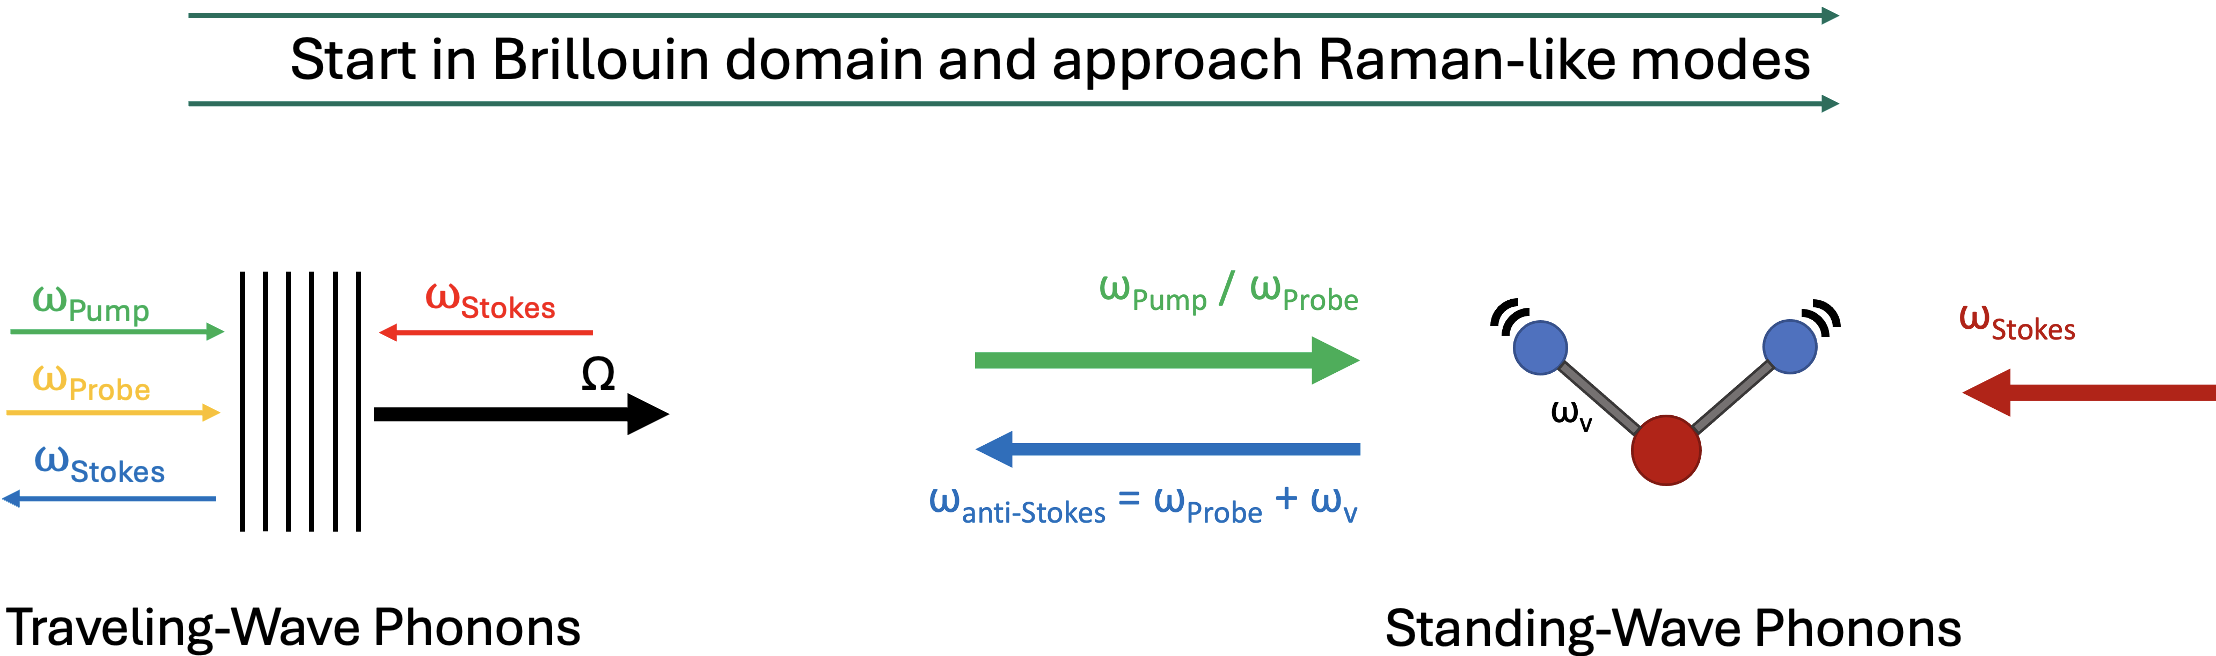
\includegraphics[width=\textwidth]{figs/4-Raman/ExploreBrillouinRamanTransition.png}
  \vspace{0.5em}
  \caption[Conceptual illustration of the transition from a traveling acoustic wave to standing-wave vibrational modes.]{Conceptual illustration of the transition from a traveling acoustic wave to standing-wave vibrational modes. In a bulk material or extended media (left), light scatters from a continuum of traveling acoustic waves (Brillouin scattering), whereas in the molecular vibrations of atomic bonds (right), only discrete standing-wave phonon modes are allowed (Raman-like scattering). The left diagram is a conceptual visualization of the \acs{CoBS} process for a longitudinally-traveling phonon \(\Omega\) (see Chapter~\ref{ch:CoBS}) while the right diagram gives a conceptual visualization of an analogous \ac{CARS} process with the standing-vibrations \(\omega_{\rm v}\) among bonded atoms in a molecule.}
  \label{fig:Raman:BrillouinRamanTransition}
\end{figure}

\subsection{Brillouin-Induced Raman Modes}
\label{subsec:Raman:Brillouin-InducedRamanModes}

In a traditional SBS experiment, a pump laser drives an acoustic wave through electrostriction, and the scattered Stokes light is down-shifted by the acoustic frequency \(f_{\rm B}\), given by \cite{boyd2020nonlinear}

\begin{equation}
  f_{\rm B} = \frac{2v_{\rm s}n}{\lambda},
  \label{eq:Raman:f_B}
\end{equation}
\\
where \(v_{\rm s}\) is the longitudinal sound speed, \(n\) is the refractive index, and \(\lambda\) is the optical frequency. In an unbounded or extended medium, the frequency response of the scattered light is determined by material properties (sound speed and optical dispersion) and the acoustic wave can be thought of as a traveling grating moving through the medium. If the medium is shortened such that the acoustic wave can reflect off the sample boundaries, the traveling acoustic waves can auto-interfere to form a standing-wave pattern in the medium. Under these system conditions, a phonon induced by \ac{SBS} will propagate to the sample end, reflect (assuming a high acoustic impedance mismatch at the boundary), and retraverse the medium in the reverse direction. If the length \(L\) between acoustic interfaces is a half-integer number of acoustic wavelengths, the forward- and backward-traveling phonon waves can interfere to form a standing wave pattern (i.e., a resonance), in essence trapping the traveling phonon in the cavity defined by the sample. This standing wave in turn acts like a stable grating, enhancing the scattering of light at well-defined frequencies corresponding to its resonances. We term these resonant phonon excitations ``Brillouin-induced Raman modes'' to reflect their hybrid character.

In more concrete terms, the finite-length system behaves like an acoustic Fabry–Pérot cavity. For a longitudinal acoustic mode, the condition for a standing wave is that an integer number \(n\) of half-wavelengths equals the round-trip length: \(\frac {n\lambda_{\rm s}}{2} = L\). Equivalently, the allowed acoustic frequencies are

\begin{equation}
  f_{\rm R} = \frac{n\,v_{\rm s}}{2L},
  \label{eq:Raman:f_R}
\end{equation}
\\
where \(v_{\rm s}\) is the sound velocity in the medium and \(n = 1, 2, 3, \dots\) indexes the mode order. The lowest-frequency mode (\(n = 1\)) has a fundamental frequency \(f_{\rm 1} \approx \frac{v_{\rm s}}{2L}\), and higher modes are integer multiples of this fundamental (assuming a simple one-dimensional confinement). Thus, instead of a single Brillouin shift \(f_{\rm B}\), one expects a ladder of equally spaced phonon modes in the scattering spectrum, resembling a Raman vibrational progression. The spacing \(\Delta f\) between adjacent modes is approximately \(\Delta f \approx \frac{v_{\rm s}}{2L}\), set solely by the cavity length and sound speed. Figure~\ref{fig:Raman:GeometryDeterminesFundamentalFreq} illustrates why this is so. For example, if \(L =\) \SI{10}{\milli\meter} in a medium where \(v_{\rm s} =\) \SI{5000}{\meter\per\second}, the fundamental mode would be \(f_{\rm 1} \approx\) \SI{250}{\kilo\hertz} and overtones at \SI{500}{\kilo\hertz}, \SI{750}{\kilo\hertz}, etc. In principle, a sufficiently short and high-Q acoustic cavity could produce a comb of multiple \si{\giga\hertz}-range lines (analogous to molecular vibrational Raman lines) out of what would ordinarily be a single broad Brillouin gain peak.

\begin{figure}[t]
  \centering
  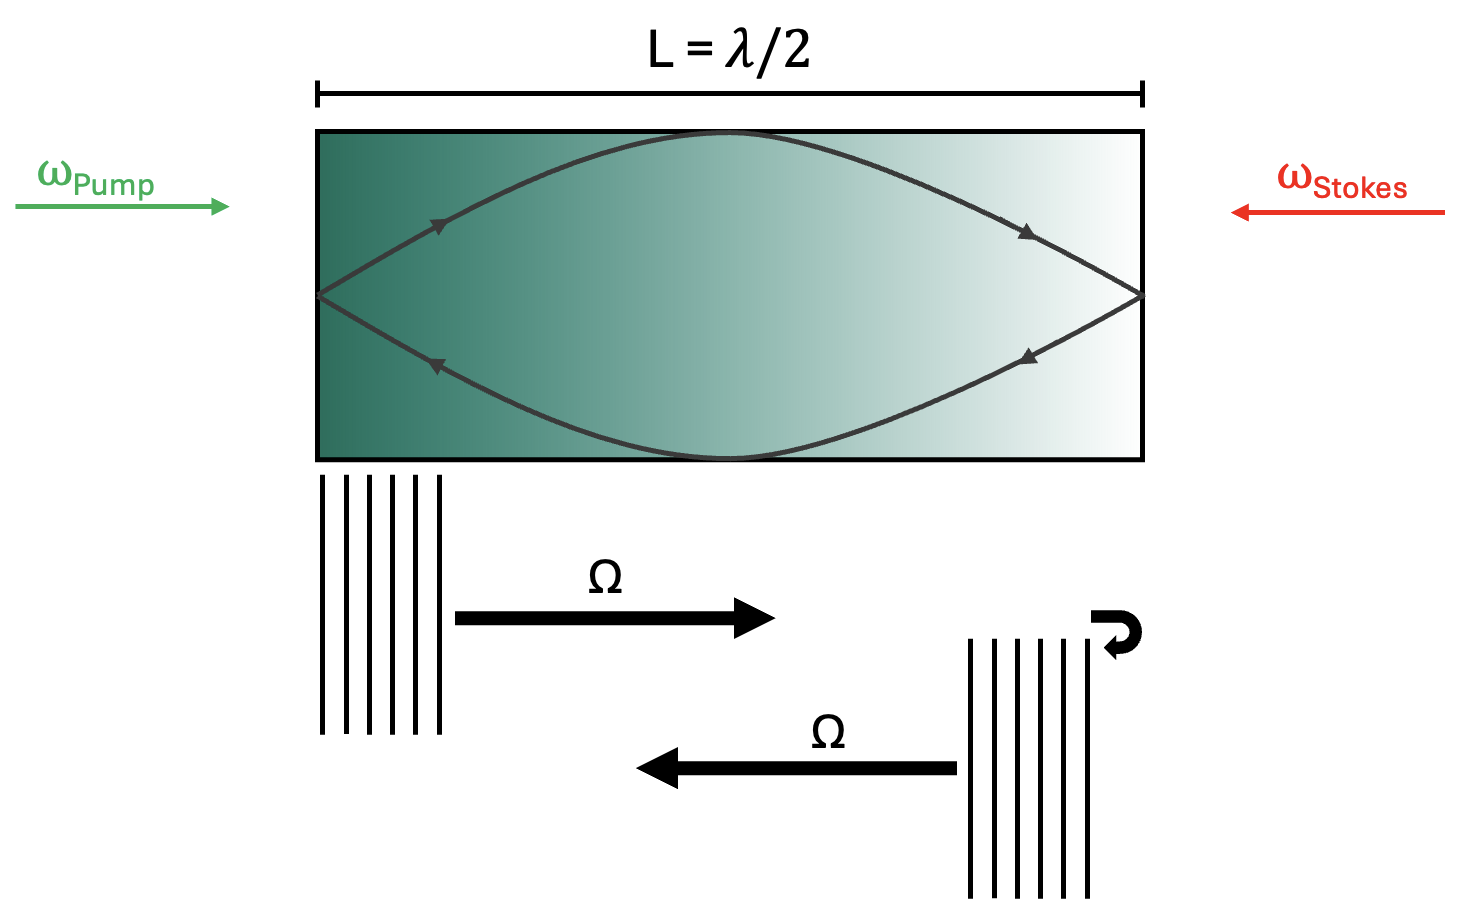
\includegraphics[width=.85\textwidth]{figs/4-Raman/GeometryDeterminesFundamentalFreq.png}
  \caption[Illustration showing how geometry and sound speed of the material determine the allowed acoustic frequencies.]{Illustration showing how geometry and sound speed of the material determine the allowed acoustic frequencies, given by Equation~\ref{eq:Raman:f_R}. Traveling-wave phonons around the material's Brillouin frequency shift \(f_{\rm B}\) are transduced within the medium via the \ac{CoBS} process. These phonons traverse the length to reach the boundary, where a high acoustic impedance mismatch causes them to reflect at the interface and retraverse the length of the medium in the reverse direction. The spatio-temporal overlap of counterpropagating traveling-wave phonons causes them to interfere, creating an acoustic standing-wave pattern within the material at discrete frequencies determined by the length and sound speed of the material. Shown in the illustration is the half-wavelength fundamental (\(n=1\)) mode, however in general, harmonics near the material's mechanical resonance frequency \(f_{\rm B}\) would be excited in the medium.}
  \label{fig:Raman:GeometryDeterminesFundamentalFreq}
\end{figure}

These Brillouin-induced modes would manifest as distinct peaks in the spectrum of the scattered light. In addition to the usual broadened Brillouin spectrum (with width given by acoustic damping), one would see a series of sharp lines at \(f_{\rm 1}, f_{\rm 2}, f_{\rm 3}, \dots\) around the center scattered frequency. Such a spectrum would be clear evidence that the phonon field is not only a freely propagating wave but also oscillating in discrete standing patterns (i.e., an optically driven acoustic resonator within the material). This is conceptually similar to stimulated Raman scattering in a molecule, where one can get a cascade of Stokes lines corresponding to \(1\hbar\omega_{\rm vib}\), \(2\hbar\omega_{\rm vib}\), \(3\hbar\omega_{\rm vib}\) energy shifts if the pump is intense. Here the ``molecular vibration'' is replaced by an acoustic cavity mode. If the pump power is high enough to drive the acoustic mode into the nonlinear regime, one might even observe multiple orders of Stokes (and anti-Stokes) as the phonon population builds up in those modes.

The idea of \ac{SBS}-driven acoustic modes has parallels in prior work. In the cryogenic experiment of Renninger et al. mentioned earlier, \cite{renninger2018bulk} a bulk acoustic mode was driven via Brillouin scattering in a \si{\centi\meter}-scale quartz crystal. At low temperatures, they observed ultra-narrow acoustic resonances (indicative of discrete modes) in place of a broad Brillouin response, confirming that acoustic coherence across the entire sample can indeed produce a modal spectrum. In our case, we seek to do this at room temperature by engineering a shorter effective acoustic cavity. We aim to accomplish this by taking advantage of our Coherently stimulated Brillouin Spectrometer (\ac{CoBS}), which offers \(\sim\)\(10^{6}\) improvement in scattered power for \(\sim\)\si{\centi\meter} lengths over traditional \ac{SBS} (see Appendix~\ref{appendix:comparison} for a comparison of scattered power across Brillouin techniques, and specifically Figure~\ref{fig:SponBSvsStimBSvsCoBS} for a comparison by effective length \(L\)).

\subsection{Key Parameters and Feasibility}
\label{subsec:Raman:KeyParametersandFeasibility}

Observing Raman-like standing-wave modes via \ac{SBS} hinges on several key parameters of the system. We identify three especially critical factors: (1) the scattered power, determined by the effective material Brillouin gain and length as well as the optical powers; (2) the acoustic dissipation in the medium, which limits the mean phonon travel distance (coherence length); and (3) the acoustic boundary reflectivity, determined by impedance mismatch at interfaces, which enables the phonons to reflect and form standing-waves. These parameters together determine whether the phonon will remain a distributed traveling excitation or collapse (blur) into discrete modes. Chapter~\ref{ch:CoBS} describes the \ac{CoBS} instrument, showing that the scattered power as a result of the \ac{CoBS} process is given by Equation~\ref{Eq:Theoretical Framework:Scattered Power}, stated here again as

\begin{equation}
  P_{\rm Signal} = \frac{1}{4}(G_{\rm B}L)^{2}P_{\rm Pump}P_{\rm Stokes}P_{\rm Probe}\Phi,
  \label{eq:Raman:ScatteredPowerPhi}
\end{equation}
\\
where \(G_{\rm B}\) is the material-dependent effective (acousto-optic overlap-adjusted) Brillouin gain factor given by Equation~\ref{Eq:Effective Brillouin Gain}, \(L\) is the effective length, \(P_{\rm i}\) are the optical powers of the pump, Stokes, and probe waves, respectively, and \(0 < \Phi < 1\) is a phase-matching relaxation term (given by Equation~\ref{Eq:Phi}) that captures the pump-probe detuning on which the instrument relies (in general, \(\Phi\) increases for smaller \(L\)). A material’s Brillouin gain coefficient \(g_{\rm 0}\) (\si{\watt\per\meter}), or overlap‐adjusted effective gain \(G_{\rm B}\) (\si{\per\watt\per\meter}), sets how strongly the phonons are driven for given \(P_{\rm Pump}\), \(P_{\rm Stokes}\), and \(P_{\rm Probe}\) optical powers over an interaction length \(L\) in the \ac{CoBS} process (see Chapter~\ref{ch:CoBS}, and specifically Equation~\ref{Eq:Theoretical Framework:Scattered Power}), given here again by

\begin{equation}
  G_{\rm B} = \frac{g_{0}}{A_{\rm eff}^{\rm ao}}\frac{\left(\frac{\Gamma_{\rm B}}{2}\right)^{2}}{\left(\Omega - \Omega_{\rm B}\right)^{2} + \left(\frac{\Gamma_{\rm B}}{2}\right)^{2}}.
  \label{eq:Raman:GB}
\end{equation}
\\
Here, \(\Gamma_{\rm B}\) is the angular Brillouin linewidth, \(\Omega\) (\(\Omega_{\rm B}\)) is the (resonant) angular acoustic frequency, \(A_{\rm eff}^{\rm ao}\) is the effective area (acousto-optic mode overlap), and \(g_{0}\) is the Brillouin gain coefficient given by

\begin{equation}
  g_{0} = \frac{\gamma_{\rm e}^{2}\omega^{2}}{nv_{\rm s}c^{3}\rho_{0}\Gamma_{\rm B}},
  \label{eq:Raman:g0}
\end{equation}
\\
where \(\gamma_{\rm e}\) is the electrostrictive constant, \(\omega\) is the angular optical frequency, \(n\) is the refractive index, \(v_{\rm s}\) is the speed of sound in the material, \(c\) is the speed of light, and \(\rho_{0}\) is the mean density of the material. Short samples demand very high effective Brillouin gain to achieve significant scattered power in a small \(L\). Certain tellurium‐based materials, for instance, can offer gain factors orders of magnitude higher than silica, \cite{sanghera2010nonlinear, abedin2005observation} allowing measureable scattered power in sub‐\si{\milli\meter} cavities. Figure~\ref{fig:Raman:GainofRelevantMaterials} shows a graphic which summarizes key gain parameters for the materials investigated in this study, including germanium-doped fiber (\acs{UHNA3}), tellurium dioxide (\ce{TeO2}), carbon disulfide (\ce{CS2}), and tellurium (\ce{Te}).

\begin{figure}[t]
  \centering
  \includegraphics[width=\textwidth]{figs/4-Raman/GainofRelevantMaterials.png}
  \caption[Brillouin gain of investigated materials.]{Brillouin gain (\(g_{0}\), \si{\meter\per\giga\watt}) and acousto-optic overlap-adjusted Brillouin gain (\(G_{\rm B} = \frac{g_{0}}{A_{\rm eff}^{\rm ao}}\), \si{\per\watt\per\meter}) of the materials investigated in this study. While the material gain (top row text) of \ac{UHNA3} fiber is \(10^{3}\) lower than the other materials, the effective area is confined tightly within its \SI{0.9}{\micro\meter} radius core, greatly improving the acousto-optic response for given length and optical power. The lenses of our free-space optical setup offer comparatively less tight confinement of the light, with the beam waist having radius \(r_{\rm Waist}=\)\SI{17}{\micro\meter} (bottom row text). The effective gain (middle row text) is ultimately the important gain parameter, as it accounts for both the material gain and the area over which light and sound interact (see Equations~\ref{eq:Raman:GB} and \ref{eq:Raman:g0}). \cite{boyd2020nonlinear, dubinskii2004teo2, johnson2023laser, behunin2015long, enright1974depolarized, coakley1975brillouin, renninger2018bulk, uchida1969elastic, schweppe1970elastic, ohmachi1972acoustic, peercy1975temperature, fleury2018non, harris1991multichannel, uchida1971optical}}
  \label{fig:Raman:GainofRelevantMaterials}
\end{figure}

Even if phonons are driven strongly, they must live long enough (i.e., have a low enough dissipation rate, or high enough acoustic \(Q = \frac{\Omega_{\rm B}}{\Gamma_{\rm B}}\)) to form a standing wave. At room temperature, intrinsic damping can limit phonon \(Q\)s to \(\sim\)\(10^{3}\)–\(10^{4}\) in many solids, \cite{heiman1979brillouin, bucaro1974high} implying attenuation lengths of \si{\milli\meter} to \si{\centi\meter} for \si{\giga\hertz} frequencies. Ideally, the sample length \(L\) should be comparable to or less than half the attenuation length so that phonons undergo multiple round trips. This is considerably more difficult at room temperature than at cryogenic temperatures, where \(Q\)s can exceed \(10^{7}\). \cite{maris1990phonon, renninger2018bulk}

Finally, the phonon must reflect rather than escape at the boundaries. Acoustic reflection is determined by the acoustic impedance mismatch between two materials at an interface, with acoustic impedance given by

\begin{equation}
  Z_{\mathrm{ac,}\,i} = \rho_{i} v_{\mathrm{s,}\,i},
  \label{eq:Raman:acoustic impedance}
\end{equation}
\\
where \(\rho_{i}\) is the mean density and \(v_{\mathrm{s,}\,i}\) is the longitudinal speed of sound in a given material \(i\). Acoustic reflection is then given by

\begin{equation}
  R = \frac{Z_{1} - Z_{2}}{Z_{1} + Z_{2}}.
  \label{eq:Raman:acoustic reflectivity}
\end{equation}
\\
A large acoustic impedance mismatch (e.g., a free surface with air on one side) can approach nearly 100\% reflection. \cite{galliou2013extremely, auld1973acoustic} For example, the acoustic reflection between \ce{TeO2} (\(\rho \approx \SI{5670}{\kilo\gram\per\cubic\meter}\), \(v_{\rm s} \approx \SI{4260}{\meter\per\second}\)) and air (\(\rho \approx \SI{1.02}{\kilo\gram\per\cubic\meter}\), \(v_{\rm s} \approx \SI{343}{\meter\per\second}\)) is \(R = 0.999\), or 99.9\%. Smaller acoustic impedance mismatches result is lower acoustic reflection, for example \(R = 0.005\), or 0.5\% between \ce{Te} (\(\rho \approx \SI{6240}{\kilo\gram\per\cubic\meter}\), \(v_{\rm s} \approx \SI{2610}{\meter\per\second}\)) and selenium (\ce{se}) (\(\rho \approx \SI{4810}{\kilo\gram\per\cubic\meter}\), \(v_{\rm s} \approx \SI{3350}{\meter\per\second}\)). Designing the sample with two opposing highly acoustically reflective boundaries is essential to generating a Raman-like standing-wave mode in the medium. In practice, however, partial reflections at each (or even just one) end may suffice so long as the net round‐trip reflectivity is high enough to sustain a mode.

In short, we want to create a high-\(Q\) acoustic resonator inside a Brillouin-active medium at room temperature: strong enough acousto-optic driving to excite the phonons, low enough damping to maintain them, and robust boundary reflections to confine them. Meeting all of these conditions can be challenging. However, the high (\(\sim\)\SI{5}{\femto\watt}) sensitivity and unique short path length advantage of our \ac{CoBS} instrument (described in Chapter~\ref{ch:CoBS} and Section~\ref{appendix:comparison}) sparks new motivation, as it provides a novel technique tailored for observing small-scale scattering phenomenon. Feasibility estimates and initial \ac{CoBS} measurements indicate that by utilizing ultra-high-gain media such as \ce{Te} \cite{sanghera2010nonlinear, abedin2005observation} or liquid \ce{CS2} \cite{boyd2020nonlinear}, and ensuring at least one boundary is acoustically reflective, one can push toward Brillouin-induced Raman modes even under ambient conditions.

The sensitivity of our instrument, representing the minimum scattered power that may be detected, has been measured at \(P_{\rm Signal}\approx\) \SI{5}{\femto\watt} (see Section~\ref{Results:Instrument sensitivity}, and specifically Table~\ref{tab:CoBS:5fWSensitivity} together with Equation~\ref{Eq:Theoretical Framework:Scattered Power} and Figure~\ref{fig:CoBS:5fWSensitivity} for validation of this claim). Using this sensitivity value for \(P_{\rm Signal}\) we can rearrange Equation~\ref{eq:Raman:ScatteredPowerPhi} to solve for the minimum length \(L\) we can expect to observe scattering within for given optical powers, material gain, and pump-probe detuning:

\begin{equation}
  L = \frac{2}{G_{\rm B}}\sqrt{\frac{P_{\rm Signal}}{P_{\rm Pump}P_{\rm Stokes}P_{\rm Probe}\Phi}},
  \label{eq:Raman:minimumL}
\end{equation}
\\
where \(0 < \Phi < 1\) and generally increases for smaller \(L\). For \(P_{\rm Signal}\approx\) \SI{5}{\femto\watt} sensitivity and maximum optical powers \(P_{\rm Pump}P_{\rm Stokes}P_{\rm Probe}\approx\) \SI{0.25}{\cubic\watt} under typical conditions, Equation~\ref{eq:Raman:minimumL} predicts, for example, the ability to observe scattering within \(\sim\)\SI{500}{\nano\meter} of \ac{UHNA3} fiber (\(G_{\rm B,\,UHNA3}=\) \SI{0.6}{\per\watt\per\meter}). Equation~\ref{eq:Raman:minimumL} makes clear that minimizing the observable scattering length is accomplished by any of: bumping applied optical powers, improving instrument sensitivity, or choosing a higher gain scattering medium.

In what follows, we detail the experimental platforms and theoretical modeling that guided our attempts to observe discrete phonon modes in high-gain materials. Although a conclusive demonstration proved elusive, the conceptual framework is robust and provides a foundation for ongoing efforts. By shrinking the acoustic path length, maximizing phonon reflectivity, and exploiting strong \ac{CoBS} gain, one can approach the regime where traveling-wave Brillouin scattering morphs into Raman-like standing-wave modes. This pursuit effectively unifies the traveling-wave and standing-wave paradigms of light-sound interaction, providing new opportunities in cavity-free phononics, resonant optomechanics, and coherent phonon devices at room temperature.

%--------------------------------------------------------------------%

\section{Results}
\label{sec:Raman:Results}

In this section we detail results and progress toward measuring Brillouin-induced Raman modes, in chronological order of investigation. The overall approach was to start deep in the continuous Brillouin domain of longitudinally-traveling phonons in bulk material and steadily approach the discrete Raman domain by measuring incrementally shorter lengths of materials well-suited to the task. This investigative study began with user-friendly fiber-coupled lengths of \ac{UHNA3} fiber, progressed quickly to increasingly challenging free-space measurements of materials such as liquid \ce{CS2} and thin films of \ce{TeO2} and \ce{Te}, and ultimately arrived at fiber-to-chip coupling into specialized suspended waveguides. We present here both the successes along the way as well as key insights gained from setbacks, with special focus on illuminating the reasoning behind critical pivots in our investigation.

\subsection{\texorpdfstring{\ce{Ge}}{Ge}-Doped Optical Fiber}
\label{subsec:Raman:Target:UHNA3}

To begin with a clear measurement firmly in the Brillouin domain, we target (short) lengths of the well-understood \ac{UHNA3} fiber. \cite{behunin2015long} \ac{UHNA3} features a Brillouin frequency shift distinct from the \ac{SMF-28} of the apparatus (\(f_{\rm B,\,UHNA3} =\) \SI{9.18}{\giga\hertz} vs \(f_{\rm B,\,SMF28} =\) \SI{10.85}{\giga\hertz}), making it easily distinguishable from instrument background. Additionally, its small core and high \ce{Ge} concentration (\(\sim\)44 wt.\%) make for tight acousto-optic overlap (\(A_{\rm eff}^{\rm ao}\)) and good guidance of both light and sound, respectively. Figure~\ref{fig:Raman:GainofRelevantMaterials} shows the key gain figures for \ac{UHNA3}. While its material gain (\(g_{0} = \SI{0.0015}{\meter\per\giga\watt}\)) is low, the acousto-optically adjusted effective Brillouin gain (\(G_{\rm B} = \frac{g_{0}}{A_{\rm eff}^{\rm ao}} = \SI{0.60}{\per\watt\per\meter}\)) is sufficiently high allow a measurement in sub-\si{\milli\meter} lengths for typical optical powers (Equation~\ref{eq:Raman:minimumL}).

Figure~\ref{fig:Raman:UHNA3pics} shows pictures of measured \SI{1}{\centi\meter} and \SI{1}{\milli\meter} lengths of \ac{UHNA3} fiber (Figures~\ref{fig:Raman:1cmUHNA3pic} and \ref{fig:Raman:1mmUHNA3pic}, respectively) spliced into the \ac{SMF-28} of the sample stage of the \ac{CoBS} apparatus. Figure~\ref{fig:Raman:1cmUHNA3} shows the observed spectra for this \SI{1}{\centi\meter} segments of \ac{UHNA3} captured at maximum available optical powers \(P_{\rm P}P_{\rm S}P_{\rm Pr} \approx \SI{0.25}{\cubic\watt}\). The peak spectral amplitude has been normalized to unity and spectral density is expressed in Arbitrary Units for clean presentation, a standard practice which acknowledges the arbitrary nature of the optical-to-electrical conversion unique to each photodiode detector. 1\(\sigma\) uncertainties are smaller than the data point markers. Figure~\ref{fig:Raman:1cmUHNA3} showcases a replication measurement taken more recently, after orders of magnitude sensitivity and performance improvements to the \ac{CoBS} instrument, however the measurement gathered initially also represented a strong successful measurement of \SI{1}{\centi\meter} \ac{UHNA3}, prompting an advance to attempting a measurement of \SI{1}{\milli\meter} \ac{UHNA3}.

\begin{figure}[t]
    \centering
    \begin{subfigure}[b]{0.49\textwidth}
        \centering
        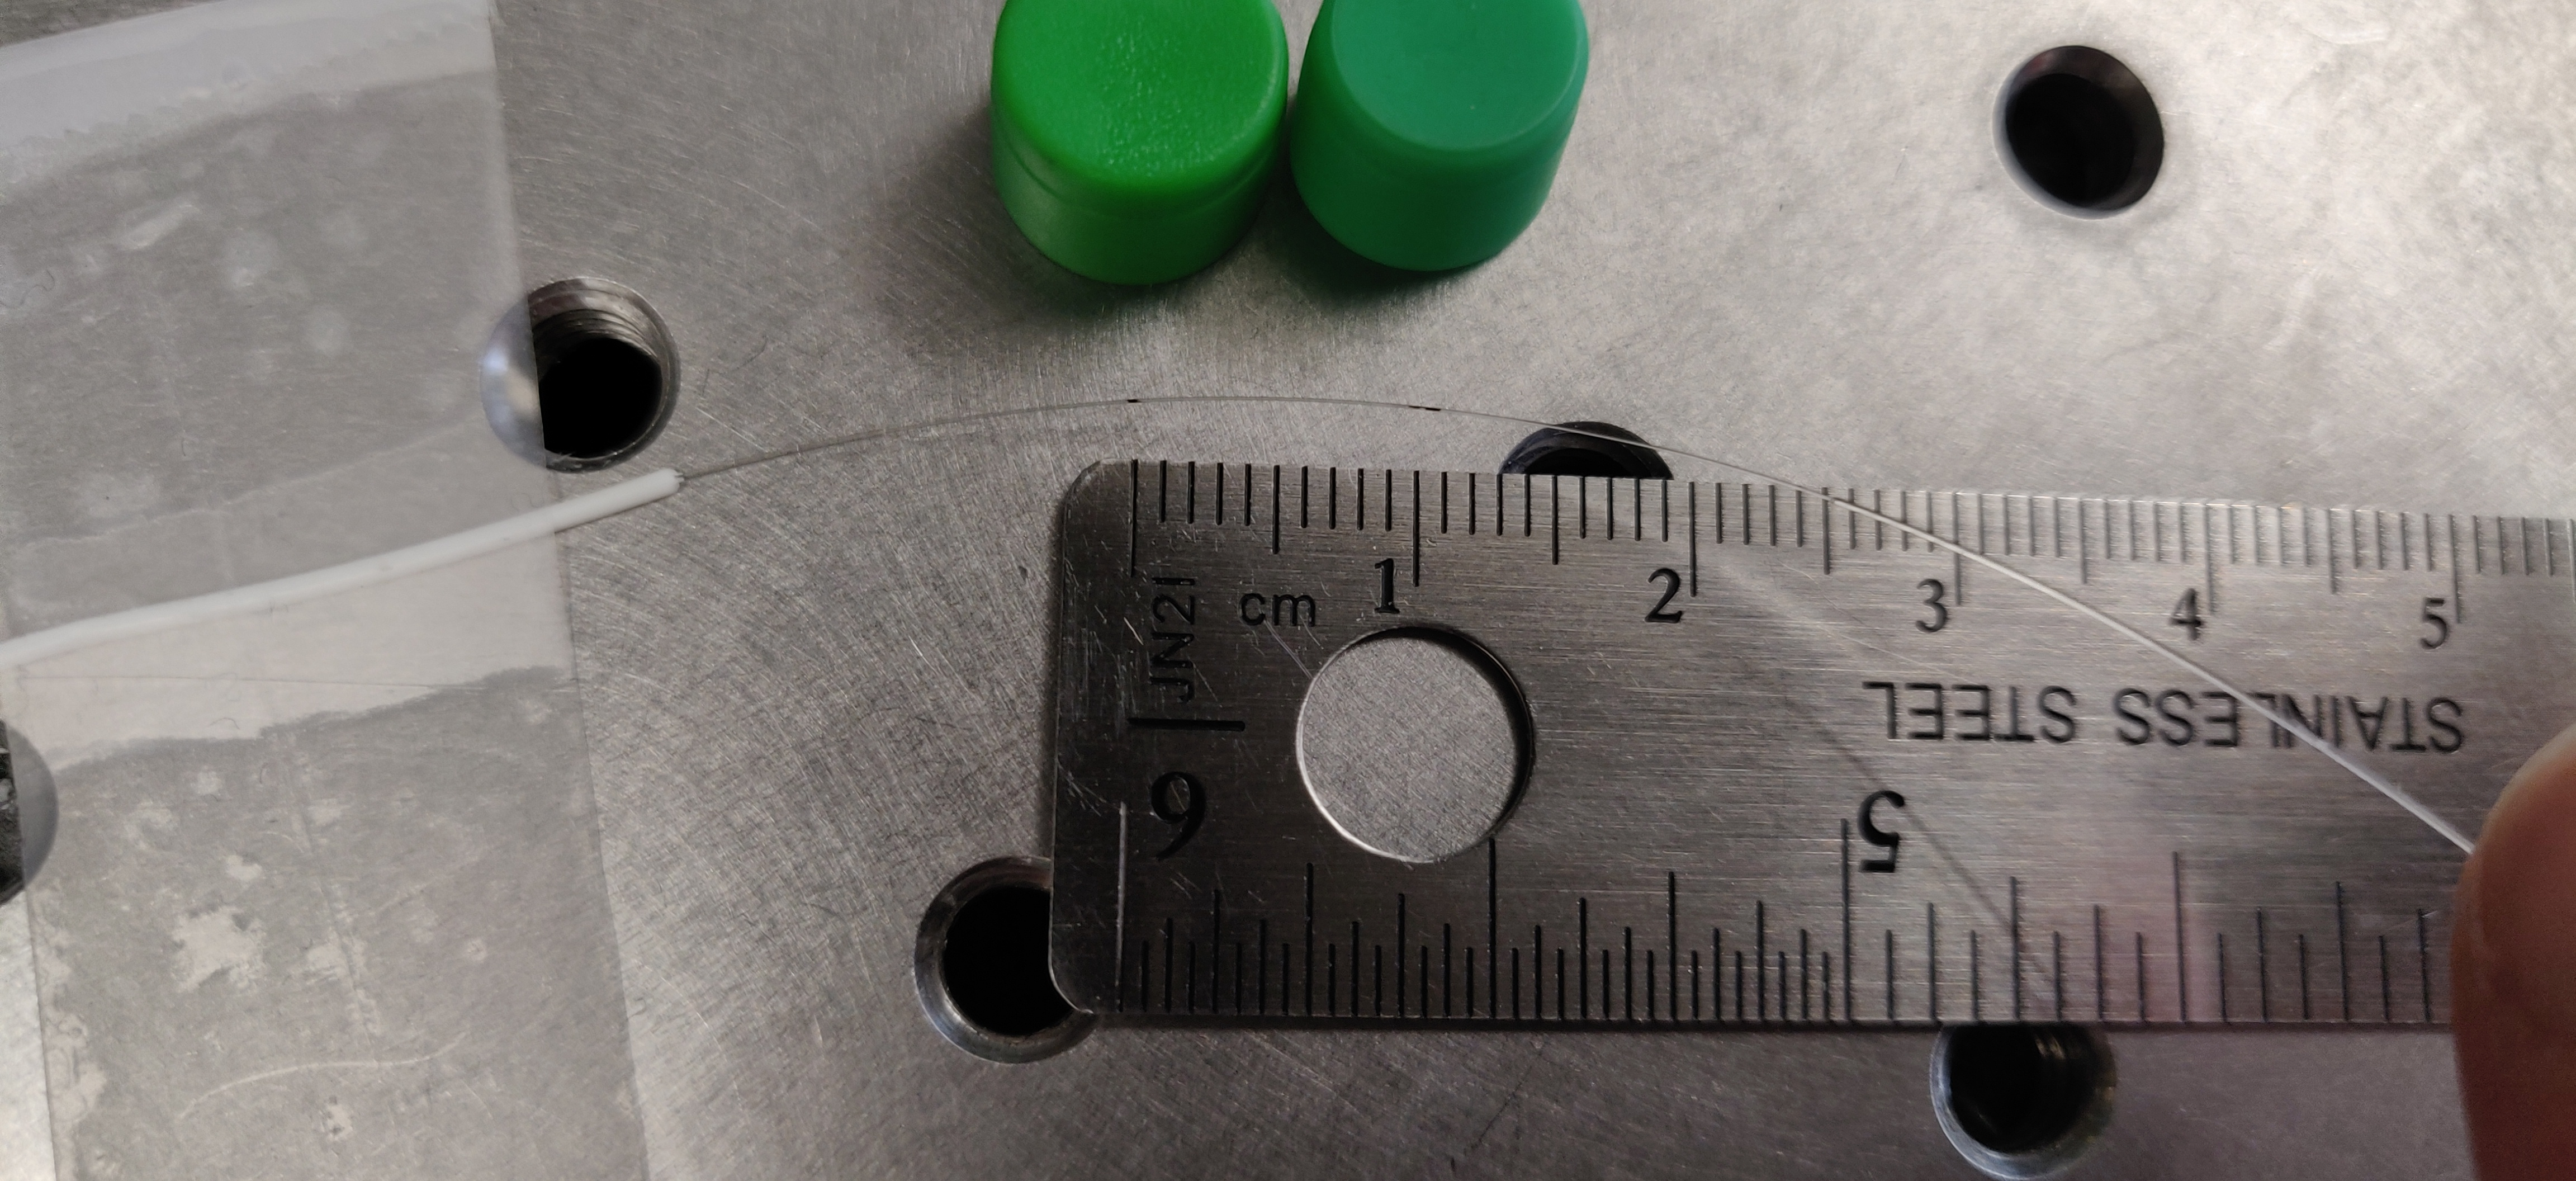
\includegraphics[width=\textwidth]{figs/4-Raman/1cm UHNA3.jpeg}
        \caption{}
        \label{fig:Raman:1cmUHNA3pic}
    \end{subfigure}
    \hfill
    \begin{subfigure}[b]{0.49\textwidth}
        \centering
        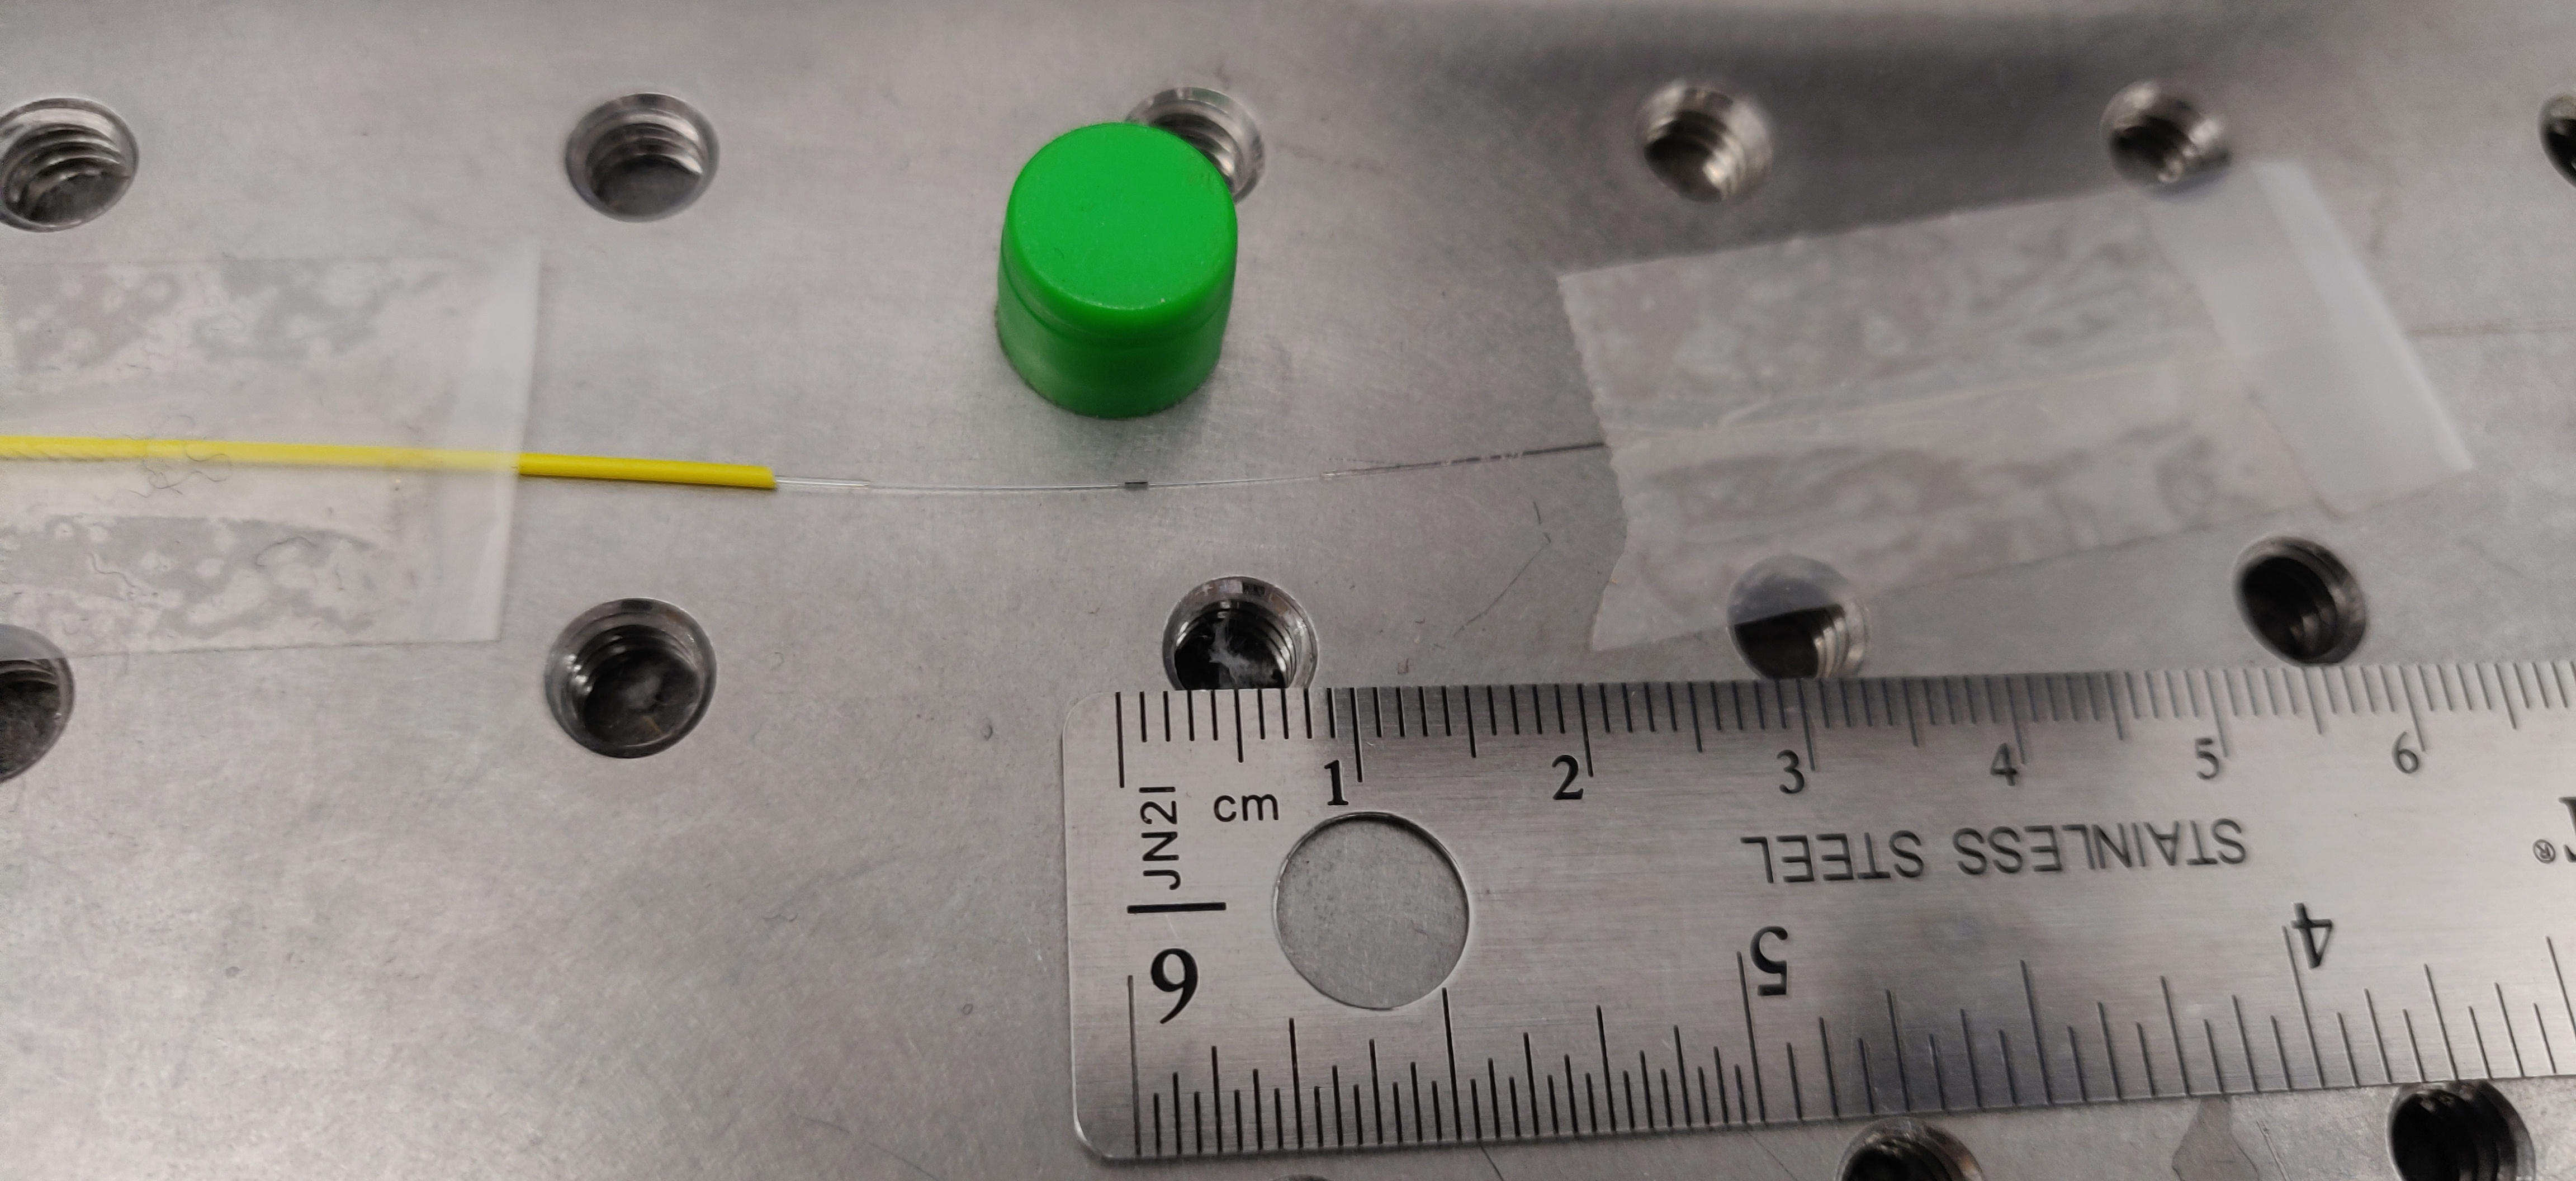
\includegraphics[width=\textwidth]{figs/4-Raman/1mm UHNA3 in apparatus.jpeg}
        \caption{}
        \label{fig:Raman:1mmUHNA3pic}
    \end{subfigure}
    \caption[Photographs of \SI{1}{\centi\meter} and \SI{1}{\milli\meter} lengths of \ac{UHNA3} fiber.]{Photographs of \textbf{(a)} \SI{1}{\centi\meter} and \textbf{(b)} \SI{1}{\milli\meter} lengths of \ac{UHNA3} fiber, indicated by black markings and spliced into the \ac{SMF-28} of the \ac{CoBS} instrument. Samples were fabricated by first splicing a longer segment of \ac{UHNA3} to \ac{SMF-28} and marking the splice location such that the \ac{UHNA3} could subsequently be cleaved to the appropriate length as measured from the marking of the first splice.}
    \label{fig:Raman:UHNA3pics}
\end{figure}

\begin{figure}[h!]
  \centering
  \begin{subfigure}[b]{0.49\textwidth}
    \centering
    \hspace{-2em}
    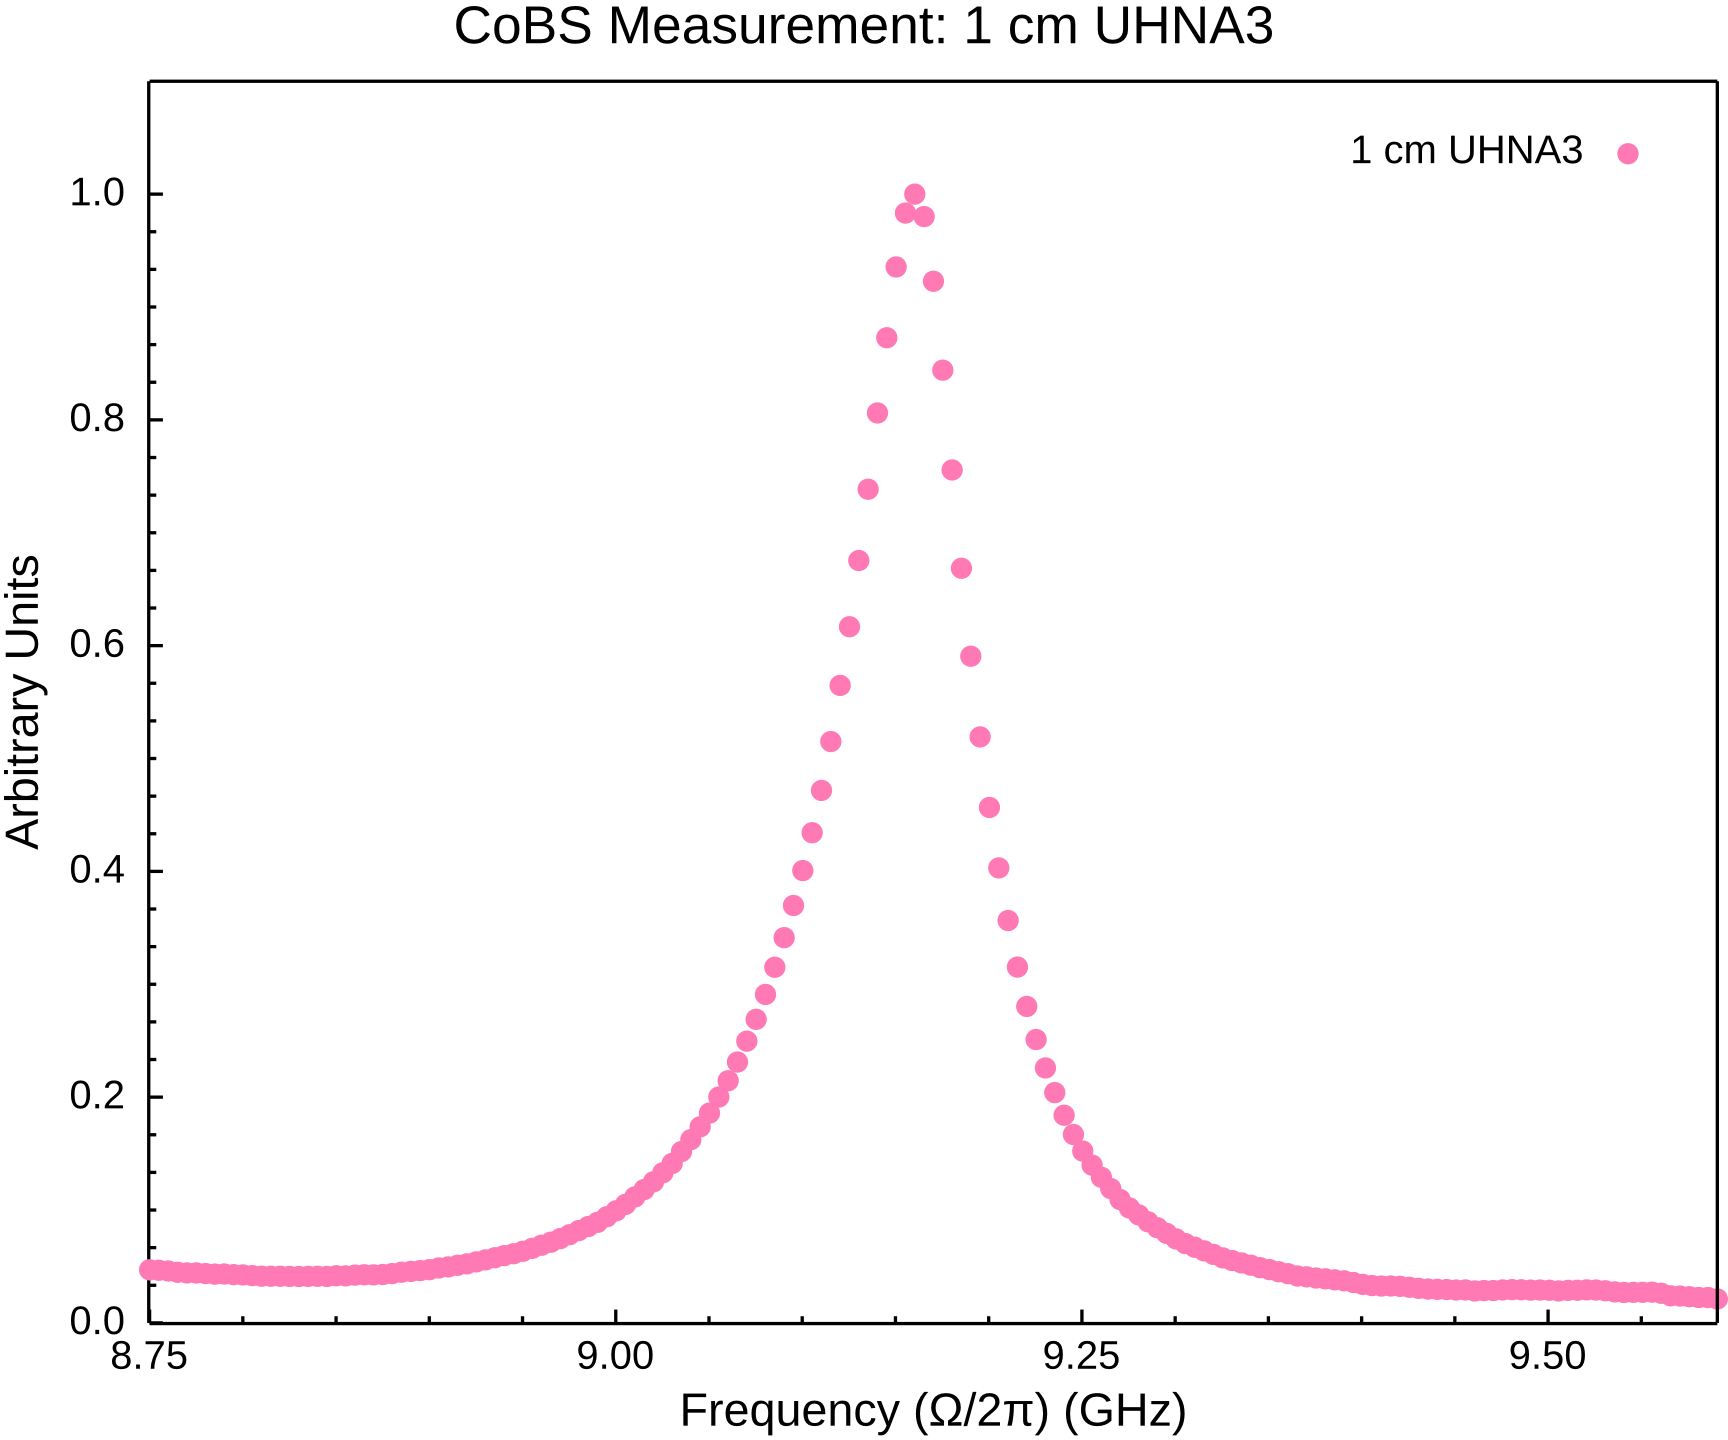
\includegraphics[width=\textwidth]{figs/4-Raman/CoBS Measurement: 1 cm UHNA3.png}
    \caption{}
    \label{fig:Raman:1cmUHNA3}
  \end{subfigure}
  \hfill
  \begin{subfigure}[b]{0.49\textwidth}
    \centering
    \hspace{-2em}
    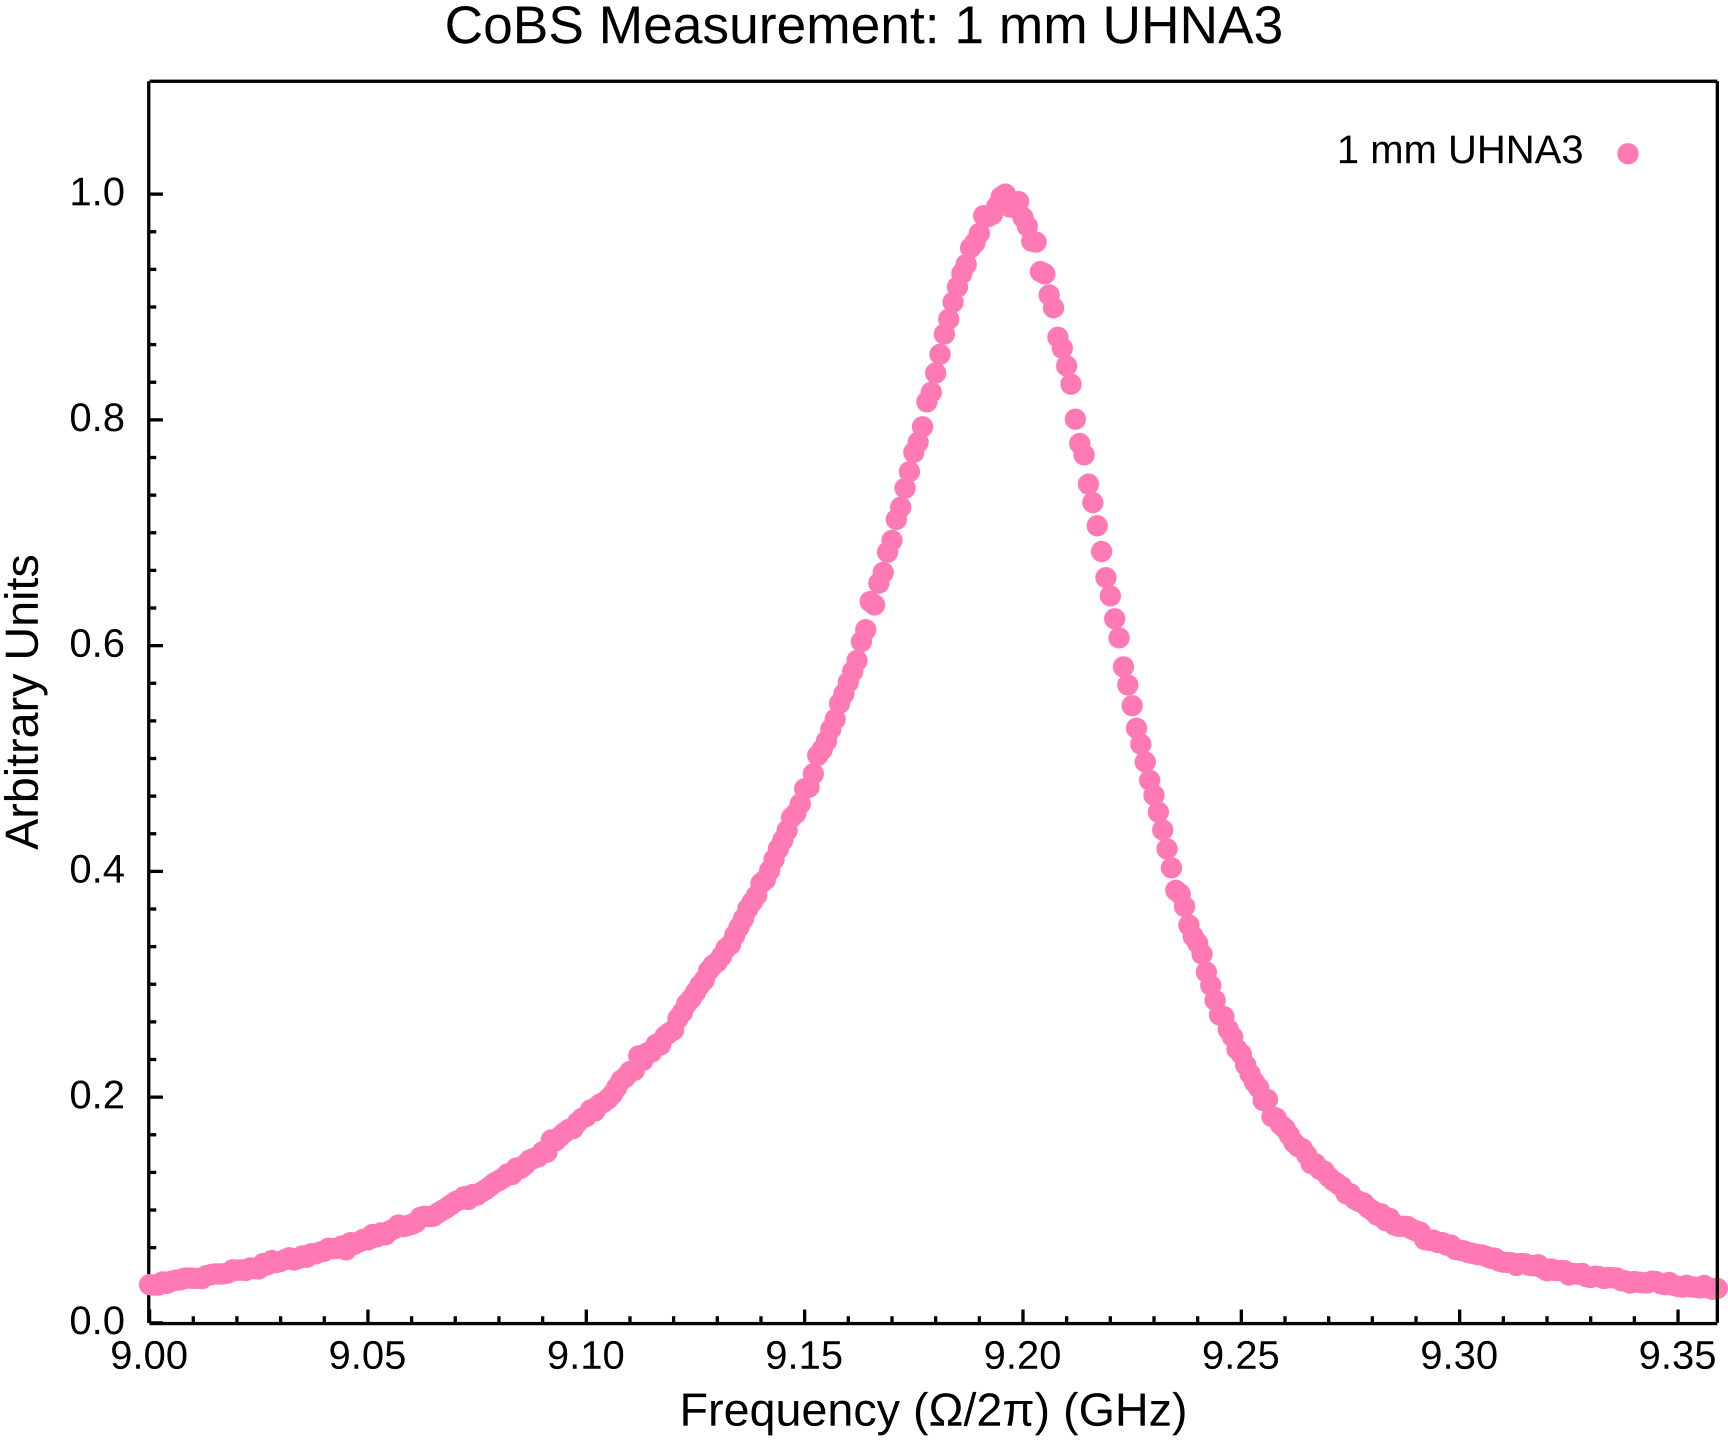
\includegraphics[width=\textwidth]{figs/4-Raman/CoBS Measurement: 1 mm UHNA3.png}
    \caption{}
    \label{fig:Raman:1mmUHNA3}
  \end{subfigure}
  \caption[\ac{CoBS} measurements of \SI{1}{\centi\meter} and \SI{1}{\milli\meter} \ac{UHNA3} fiber, in pursuit of observing Brillouin-induced Raman modes.]{Observed background-subtracted spectrum obtained through a \ac{CoBS} measurement of \textbf{(a)}~\SI{1}{\centi\meter} of \ac{UHNA3} fiber (pictured in Figure~\ref{fig:Raman:1cmUHNA3pic}) and \textbf{(b)}~\SI{1}{\milli\meter} of \ac{UHNA3} fiber (pictured in Figure~\ref{fig:Raman:1mmUHNA3pic}), captured at maximum operating optical powers \(P_{\rm P}P_{\rm S}P_{\rm Pr} \sim \SI{0.25}{\cubic\watt}\), with 1\(\sigma\) uncertainties smaller than the data point markers. The spectrum shows strong Fano asymmetry (see Section~\ref{Appendix:Fano} in Appendix~\ref{appendix: CoBS}), indicating interference of a weak signal with the broad background continuum. This is an older measurement, taken prior to orders of magnitude sensitivity improvements, and the Fano effects seen here indicate this was near the sensitivity limit of the instrument at the time.}
  \label{fig:Raman:UHNA3}
\end{figure}

This \SI{1}{\milli\meter} \ac{UHNA3} measurement is shown in Figure~\ref{fig:Raman:1mmUHNA3}, which features slight Fano asymmetry in lineshape indicative of signal-background interference in a low-signal regime (see Section ~\ref{Appendix:Fano} in Appendix~\ref{appendix: CoBS}). Unlike Figure~\ref{fig:Raman:1cmUHNA3}, which was recaptured more recently, after orders-of-magnitude sensitivity and performance improvements to the \ac{CoBS} instrument, the spectra shown in Figure~\ref{fig:Raman:1mmUHNA3} dates to the time of its relevance to this investigation. The slight Fano asymmetry indicates that this measurement, while very clear and of high SNR, was captured from a signal which was near the order of the background continuum. This places the measurement not far from the sensitivity limit of the instrument at the time. Nonetheless, Figure~\ref{fig:Raman:1mmUHNA3} represents a clear successful measurement of \SI{1}{\milli\meter} \ac{UHNA3} fiber, prompting a continuation on the path to shorter lengths and Brillouin-induced Raman modes.

\subsection{Free-Space Optics with Liquid \texorpdfstring{\ce{CS2}}{CS2}}
\label{subsec:Raman:Target:CS2Vial}

Having exhausted the shortest practical lengths of optical fiber reasonably fabricatable, a regime change to free-space optics in the \ac{CoBS} sample stage was required to progress our investigation further. To smooth this transition, we first targeted meaningful lengths of the high-gain liquid \ce{CS2}. From Figure~\ref{fig:Raman:GainofRelevantMaterials}, \ce{CS2} has a material Brillouin gain of \(\sim\SI{1.5}{\meter\per\giga\watt}\), which is \(10^{3}\) higher than that of \ac{UHNA3} fiber, however this material advantage is offset by the much looser acousto-optic mode overlap afforded by the beam waist produced by our lenses (\(A_{\rm eff,\,Free-Space}^{\rm ao} = \pi(\SI{17}{\micro\meter})^{2}\) vs \(A_{\rm eff,\,UHNA3}^{\rm ao} = \pi(\SI{0.9}{\micro\meter})^{2}\)). The resulting effective Brillouin gain of liquid \ce{CS2} in the free-space optical setup of our \ac{CoBS} instrument is \(G_{\rm B} \approx \SI{1.65}{\per\watt\per\meter}\), nearly a factor of 3 greater than that of \ac{UHNA3}. This combined with an initially targeted length \(L = \SI{1}{\centi\meter}\) provided a sufficiently large target for a gentle transition from the fiber-coupled to free-space regime.

Figure~\ref{fig:Raman:CS2Cuvetpics} shows photographs of a \SI{1}{\centi\meter}-by-\SI{4}{\milli\meter} path length cuvet of liquid \ce{CS2} mounted in the sample stage between two lenses. Light is guided from the fiber of the apparatus into free space, collimated and focused by the fiber ports and diffraction-limited lenses on either side of the fiber bench upon which the sample sits. Figure~\ref{fig:Raman:1cmCS2pic} shows the cuvet placed in the \SI{1}{\centi\meter} path length configuration while Figure~\ref{fig:Raman:4mmCS2pic} shows it rotated \SI{90}{\degree} for the \SI{4}{\milli\meter} path length configuration.

Figure~\ref{fig:Raman:CS2Cuvet} shows the observed spectra from \ac{CoBS} measurements of \SI{1}{\centi\meter} and \SI{4}{\milli\meter} liquid \ce{CS2} photographed in Figure~\ref{fig:Raman:CS2Cuvetpics}. Both measurements showcase significant Fano asymmetry, again indicative of signal-background interference in a low-signal regime (see Section~\ref{Appendix:Fano} in Appendix~\ref{appendix: CoBS}). The strong Fano interference in both measurements emphasizes the proximity to the sensitivity limit of the \ac{CoBS} instrument at the time these spectra were observed. Each progression to lower-signal (less scattered power \(P_{\rm Signal}\), from Equation~\ref{eq:Raman:ScatteredPowerPhi}) represents iterative sensitivity and performance improvements to the \ac{CoBS} instrument, ranging from insights about the importance of well-cleaned and polished pigtail ends throughout the apparatus to operating setting discoveries such as setting both the pump and probe lasers to ``whisper'' instead of ``dither'' mode, as well as component upgrades such as a higher performance detector and higher power Erbium-doped fib er amplifiers (\acs{EDFA}s) (see Chapter~\ref{ch:CoBS} for more details on the \ac{CoBS} instrument and Section~\ref{Methods:Experimental Techniques} for specifics on performance optimization).

\begin{figure}[t]
    \centering
    \begin{subfigure}[b]{0.49\textwidth}
        \centering
        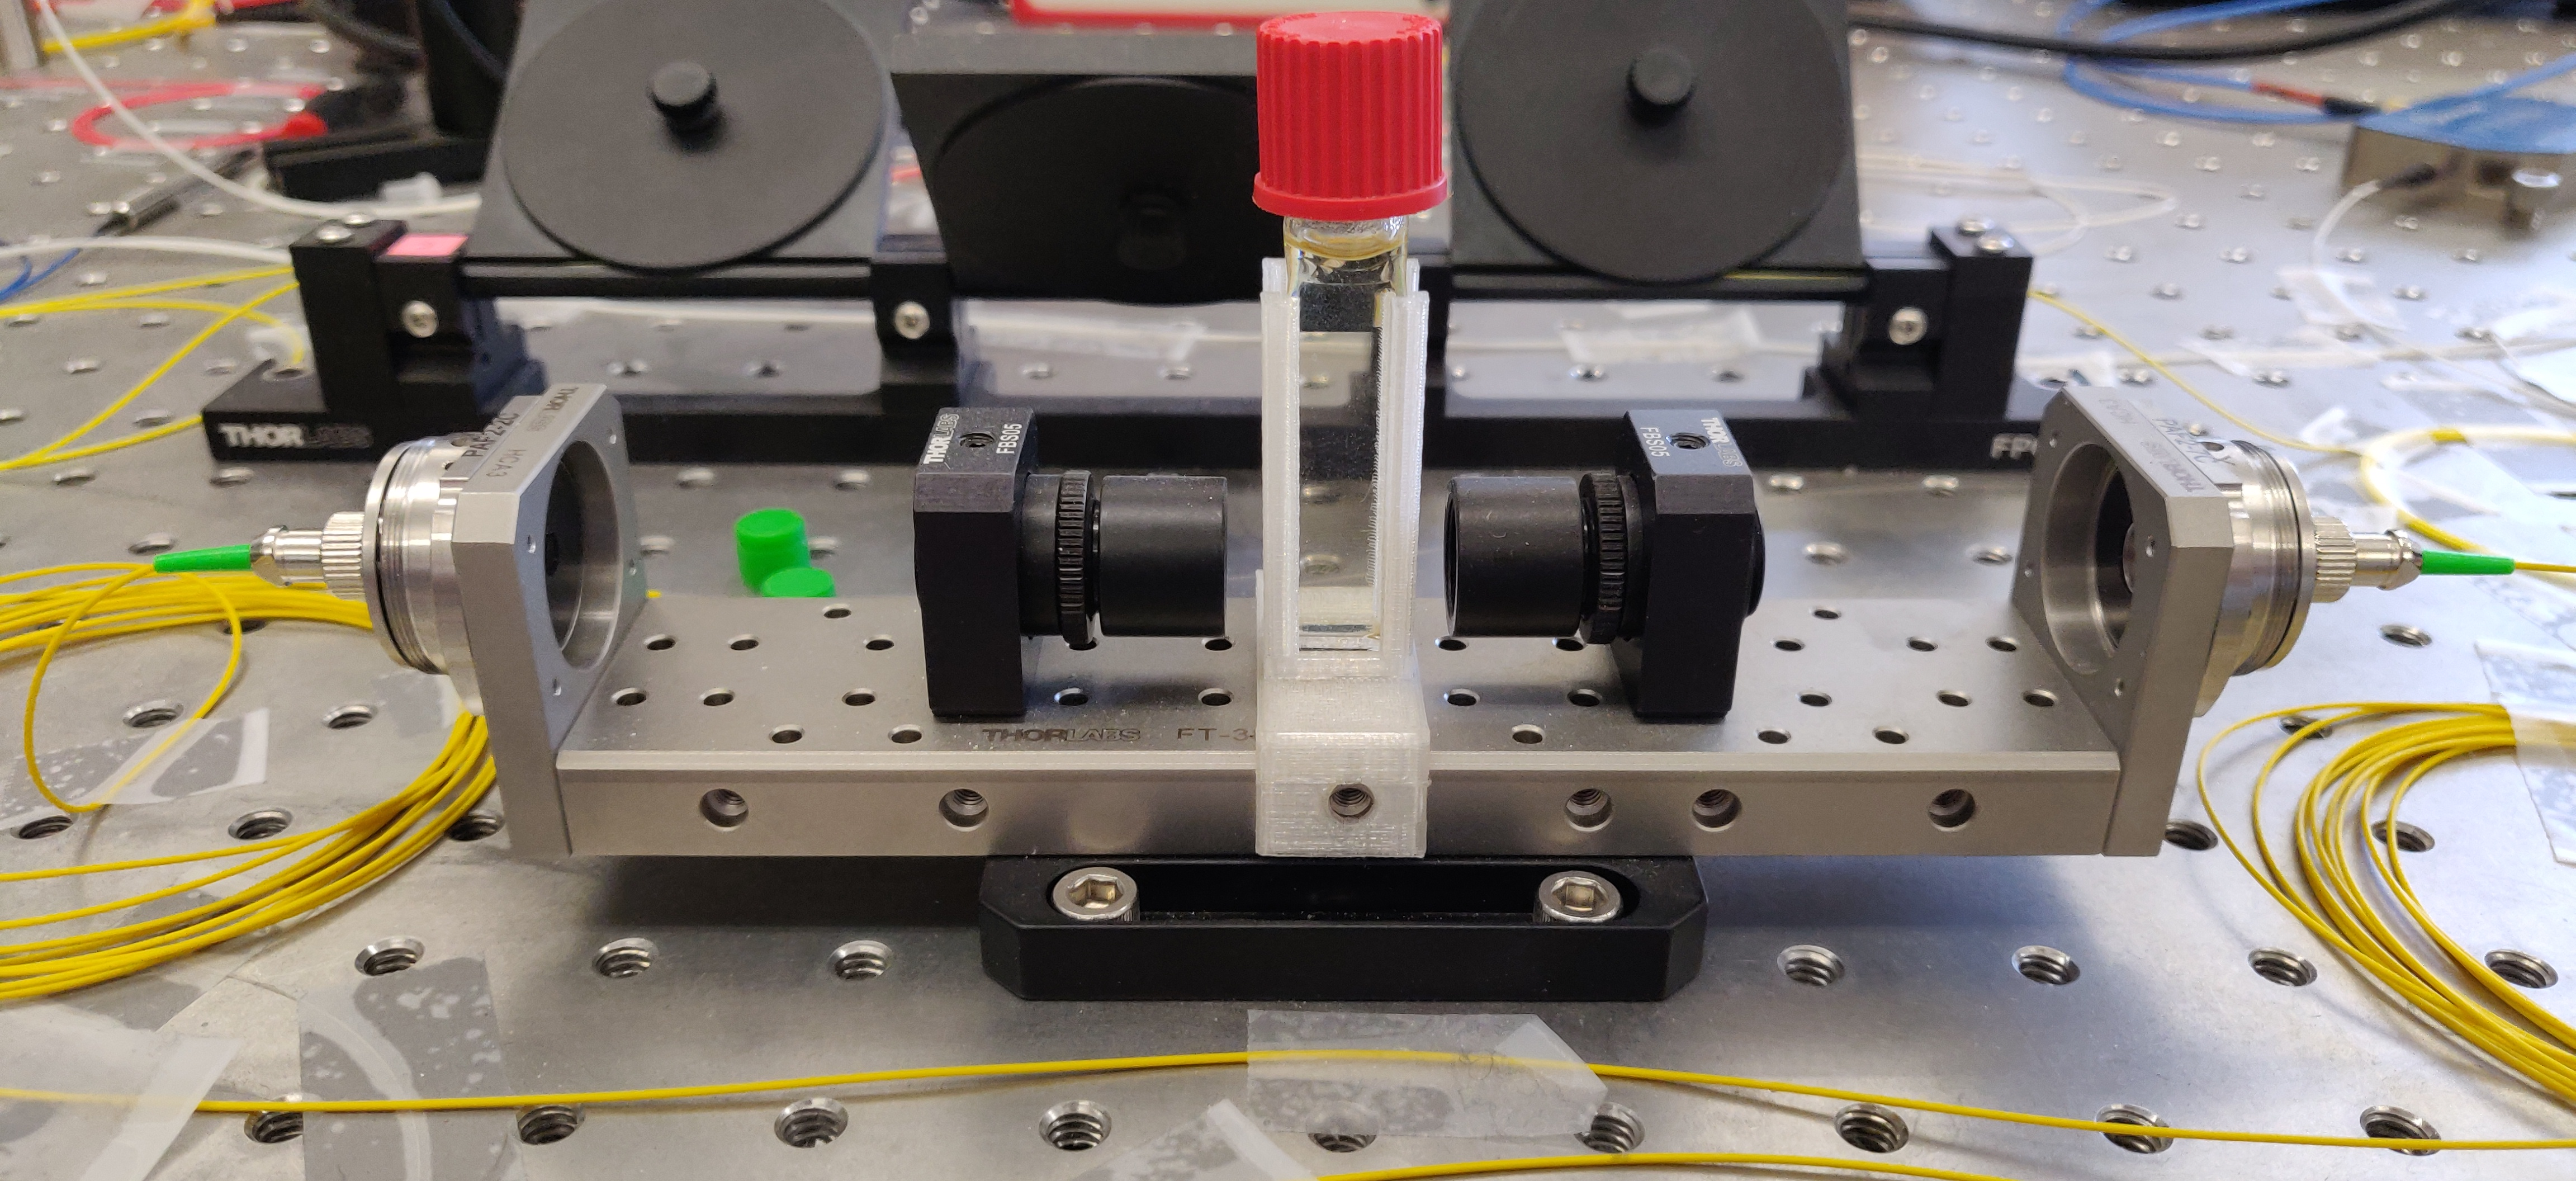
\includegraphics[width=\textwidth]{figs/4-Raman/1cmCS2.jpeg}
        \caption{}
        \label{fig:Raman:1cmCS2pic}
    \end{subfigure}
    \hfill
    \begin{subfigure}[b]{0.49\textwidth}
        \centering
        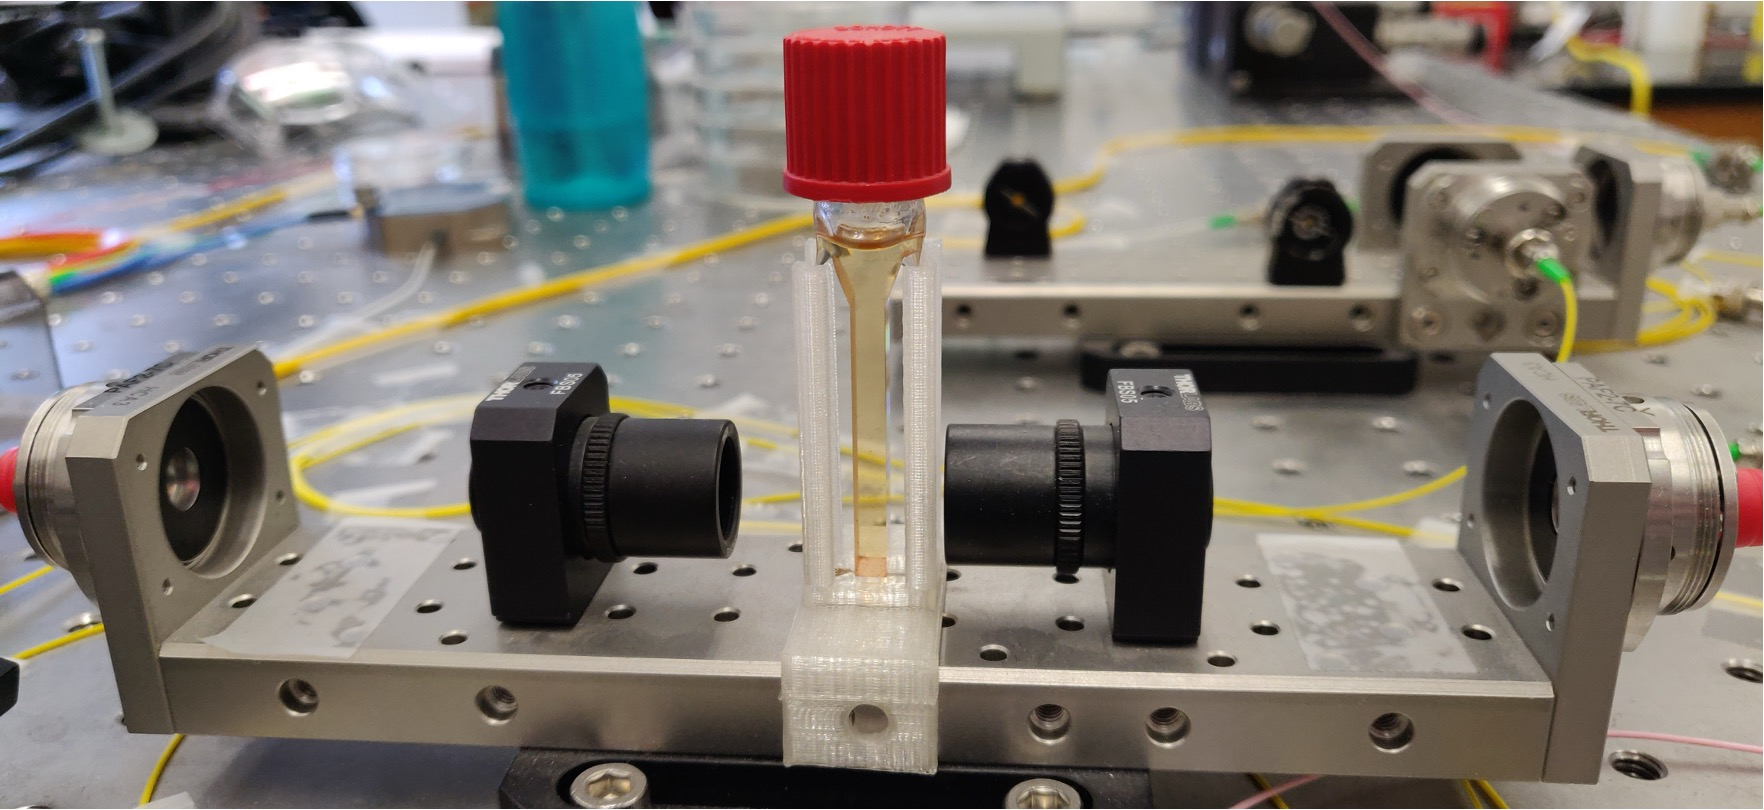
\includegraphics[width=\textwidth]{figs/4-Raman/4mmCS2.jpg}
        \caption{}
        \label{fig:Raman:4mmCS2pic}
    \end{subfigure}
    \caption[Photographs of \SI{1}{\centi\meter} and \SI{4}{\milli\meter} lengths of liquid \ce{CS2} in the beam path of the \ac{CoBS} instrument.]{Photographs of \textbf{(a)} \SI{1}{\centi\meter} and \textbf{(b)} \SI{4}{\milli\meter} lengths of liquid \ce{CS2} in the beam path of the \ac{CoBS} instrument. The single \SI{1}{\centi\meter}-by-\SI{4}{\milli\meter} path length cuvet allowed for both measurements shown in Figure~\ref{fig:Raman:CS2Cuvet} via \SI{90}{\degree} rotation within its mount.}
    \label{fig:Raman:CS2Cuvetpics}
\end{figure}

\begin{figure}[h!]
  \centering
  \begin{subfigure}[b]{0.49\textwidth}
    \centering
    \hspace{-2em}
    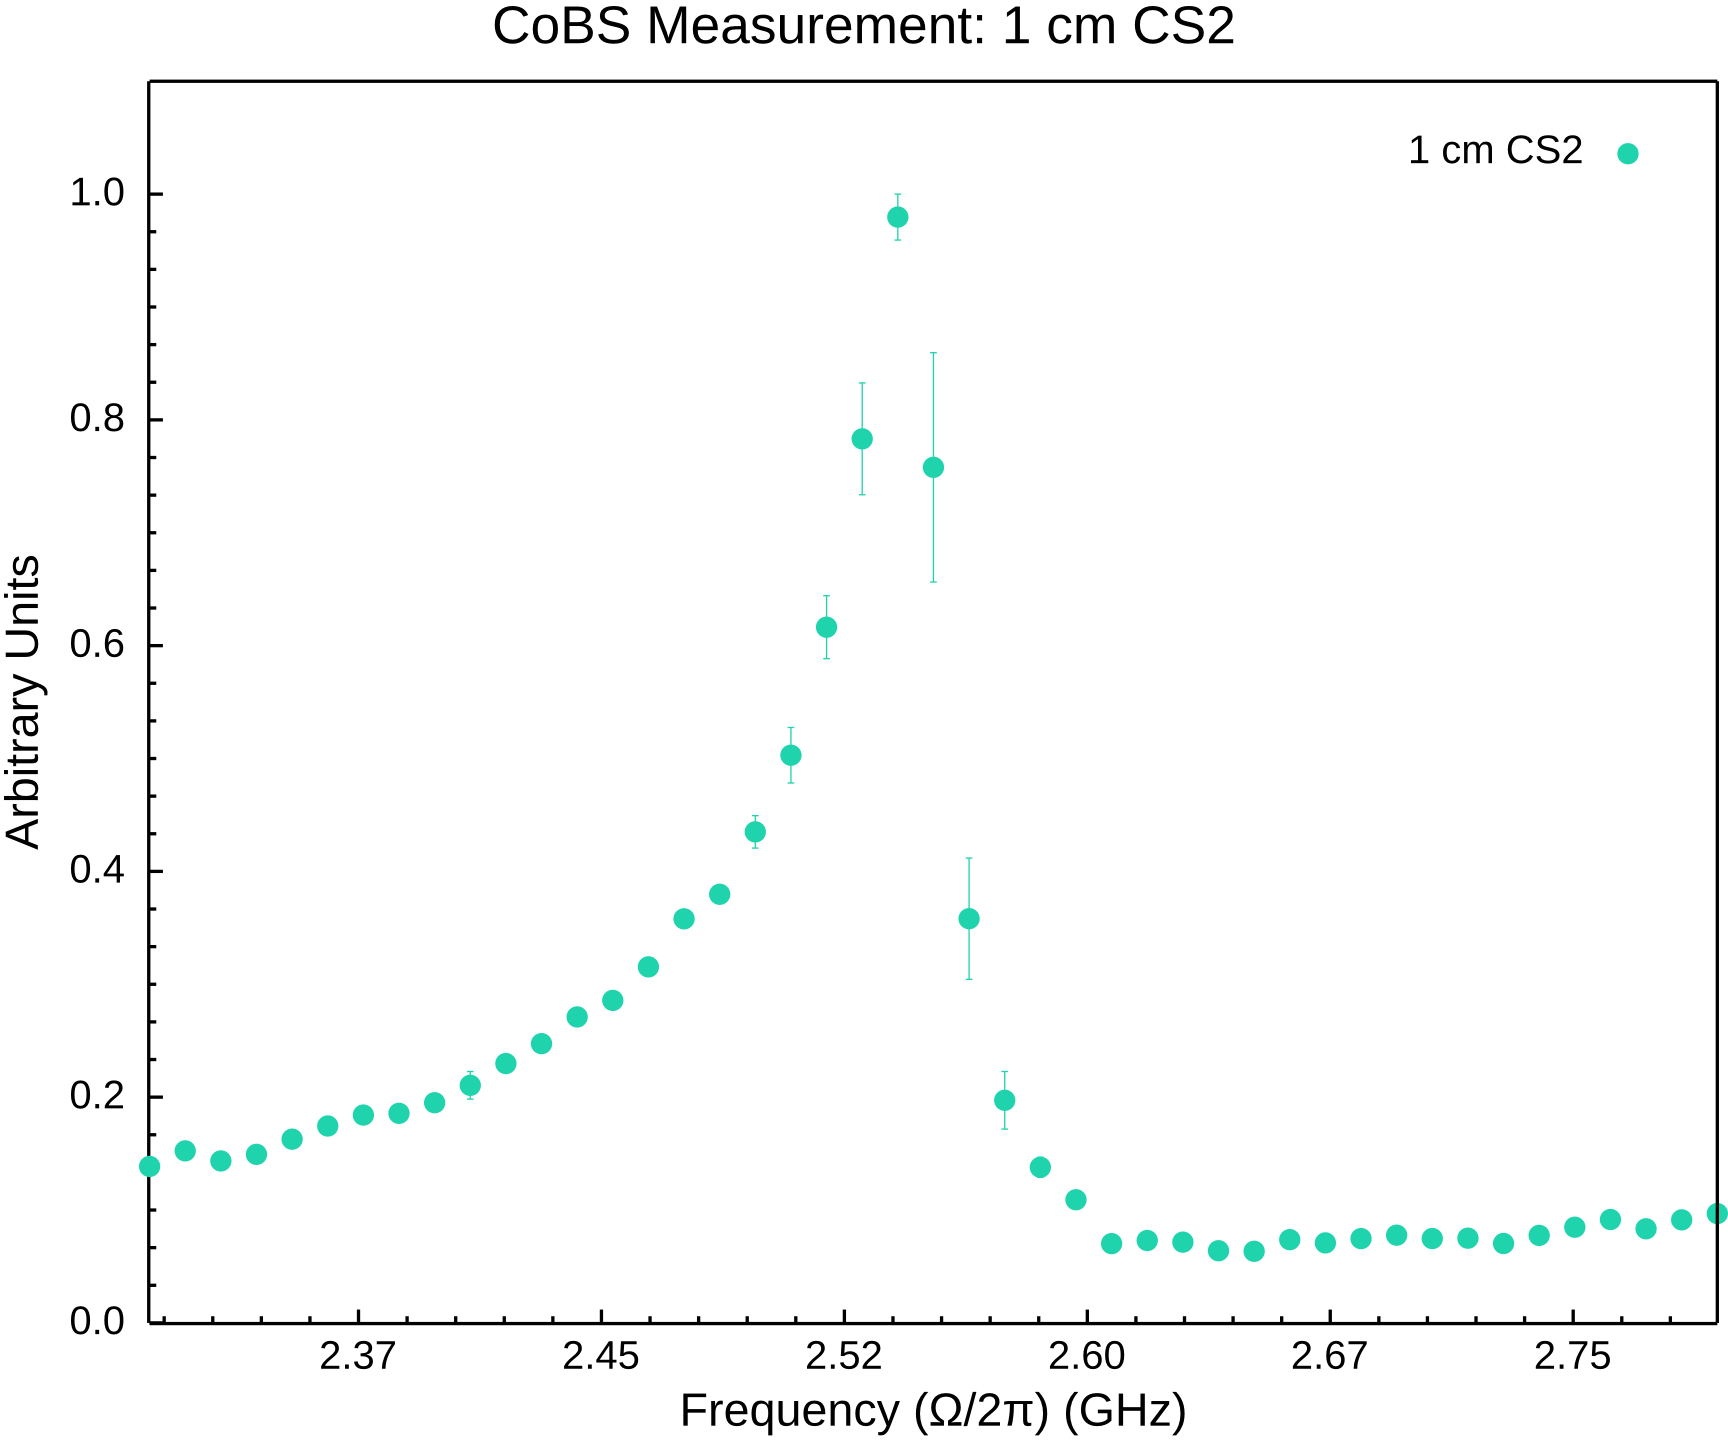
\includegraphics[width=\textwidth]{figs/4-Raman/CoBS Measurement: 1 cm CS2.png}
    \caption{}
    \label{fig:Raman:1cmCS2}
  \end{subfigure}
  \hfill
  \begin{subfigure}[b]{0.49\textwidth}
    \centering
    \hspace{-2em}
    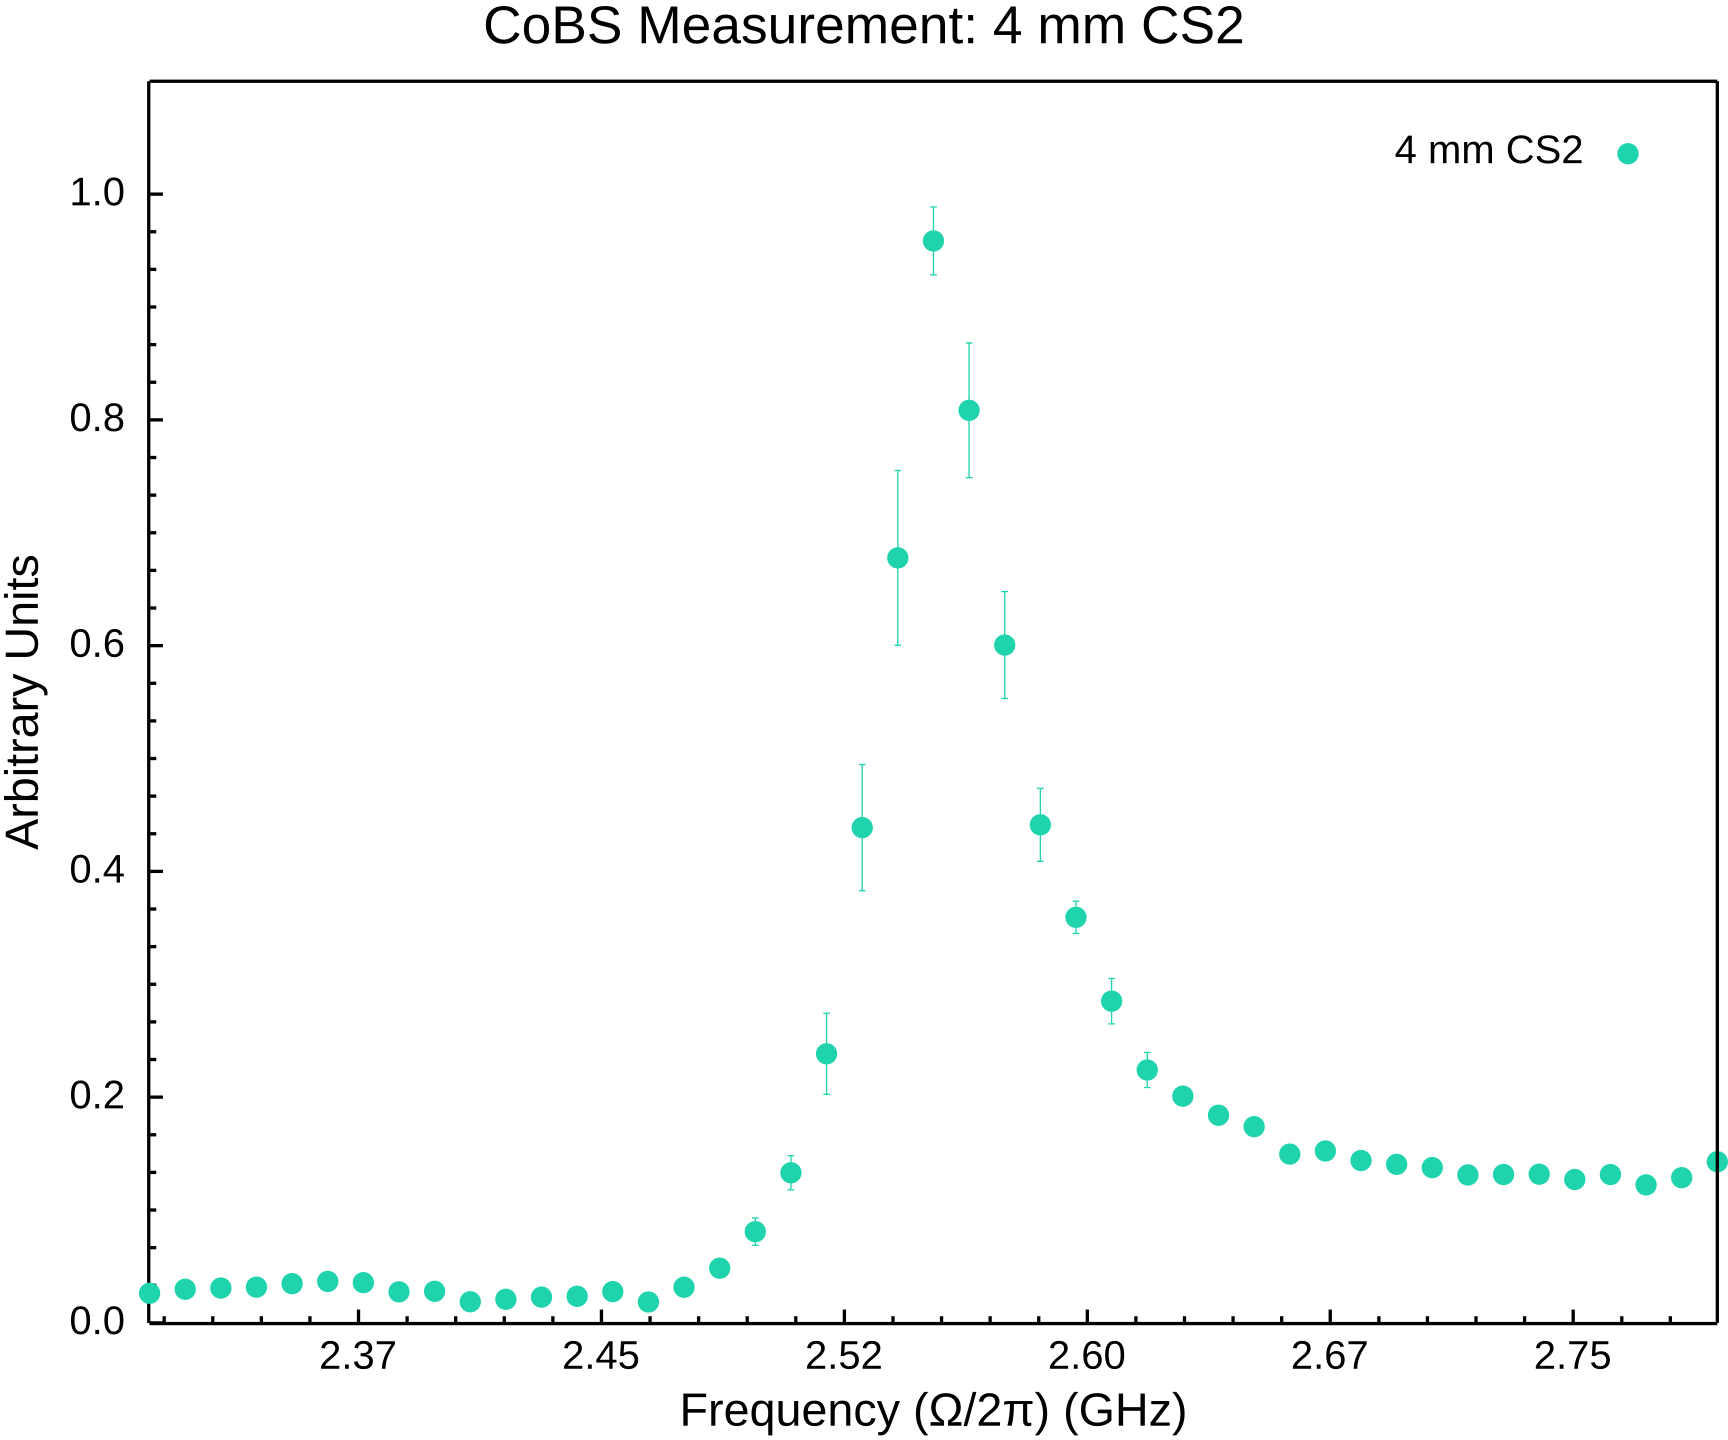
\includegraphics[width=\textwidth]{figs/4-Raman/CoBS Measurement: 4 mm CS2.png}
    \caption{}
    \label{fig:Raman:4mmCS2}
  \end{subfigure}
  \caption[\ac{CoBS} measurements of \SI{1}{\centi\meter} and \SI{4}{\milli\meter} liquid \ce{CS2}.]{Observed background-subtracted spectrum obtained through a \ac{CoBS} measurement of \textbf{(a)}~\SI{1}{\centi\meter} of liquid \ce{CS2} (pictured in Figure~\ref{fig:Raman:1cmCS2pic}) and \textbf{(b)}~\SI{4}{\milli\meter} of liquid \ce{CS2} (pictured in Figure~\ref{fig:Raman:4mmCS2pic}), with 1\(\sigma\) uncertainties smaller than the data point markers. The spectrum shows strong Fano asymmetry (see Section~\ref{Appendix:Fano} in Appendix~\ref{appendix: CoBS}), indicating interference of a weak signal with the broad background continuum. This is an older measurement, taken prior to orders of magnitude sensitivity improvements, and the Fano effects seen here indicate this was near the sensitivity limit of the instrument at the time.}
  \label{fig:Raman:CS2Cuvet}
\end{figure}

With proof-of-principle free-space functionality demonstrated with the successful measurement of \SI{1}{\centi\meter} and \SI{4}{\milli\meter} bulk liquid \ce{CS2} in a cuvet, all basic experimental infrastructure was in place to pursue Brillouin-induced Raman modes in much shorter length samples. The newly-achieved \(\sim\)\SI{10}{\femto\watt} sensitivity limit of the instrument around this time, experimentally-obtained from reduced-power measurements of \SI{1}{\centi\meter} \ac{UHNA3} fiber, supported the feasibility of measuring scattering in far shorter interaction lengths. With this in mind, we made the ambitious leap to thin films.

\subsection{\texorpdfstring{\ce{TeO2}}{TeO2} Thin Film}
\label{subsec:Raman:Target:TeO2}

Table~\ref{tab:Raman:TeO2} presents key values for material properties of \ce{TeO2} relevant to observing Brillouin-induced Raman modes for both the crystalline and amorphous thin film forms. To observe Raman-like modes in a confined medium, we must be able to sufficiently excite traveling-wave phonons via the \ac{CoBS} process in an effective length equal to at most half the mean travel distance of the phonons in that material (coherence length \(L_{\rm coh}\)). Phonon coherence length is a function of the material's mechanical dissipation rate, or Brillouin linewidth \(L_{\rm coh} = \frac{2\pi v_{\rm s}}{\Gamma_{\rm B}} = \tau_{\rm p}v_{\rm s}\), where \(\tau_{\rm p}\) is the phonon lifetime \(\tau_{\rm p} = 2\pi\Gamma_{\rm B}^{-1}\). Setting the effective length \(L\) at half of the phonon coherence length ensures the phonons make at least one round-trip in the material before dissipating (decohering), representing a critical requirement in observing Brillouin-induced Raman modes. In the table, a \ac{CoBS} scattered power estimate is given (via Equation~\ref{eq:Raman:ScatteredPowerPhi}), corresponding to half the phonon coherence length of the material. This figure (consistent for \(L_{\rm coh}/2\) and in \si{\pico\watt} reported units across all similar material property tables presented in this chapter) offers a reference for the minimum sensitivity performance required from the \ac{CoBS} instrument if Raman modes are to be observed in the material. For example, if Raman modes are to be observed in crystalline \ce{TeO2}, the effective length of the sample used to measure them must be at most \(L_{\rm eff,\,sample} = \frac{L_{\rm coh}}{2} = \SI{215}{\micro\meter}\) and \ac{CoBS} must be capable of \SI{3500}{\pico\watt} sensitivity (which it achieves by \(\sim\)\(10^{3}\)). In the table, \(\tau\) is the phonon lifetime (\(\tau = (2\pi\cdot\Gamma_{\rm B})^{-1}\)), \(v_{\rm s,\,long}\) is the longitudinal sound speed, \(n\) is the refractive index, and \(\Omega_{\rm B}\) and \(\Omega_{\rm R,\,\SI{1}{\micro\meter}}\) are the Brillouin frequency shift (Equation~\ref{eq:Raman:f_B}) and the first harmonic (\(n = 1\)) of the fundamental \(L_{0}\) Raman mode for \(L = \SI{1}{\micro\meter}\) (Equation~\ref{eq:Raman:f_R}), respectively. The reported first harmonic Raman mode is also consistent across all material property tables in this chapter as calculated for \(L = \SI{1}{\micro\meter}\).

Table~\ref{tab:Raman:TeO2} shows that to measure Brillouin-induced Raman modes in an amorphous thin film of \ce{TeO2}, the the film may be at most \(\frac{L_{\rm coh}}{2} \approx \SI{41}{\micro\meter}\) (notably beyond the standard thickness considered to be a ``thin film'') and \ac{CoBS} must be capable of \(P_{\rm CoBS,\,\frac{L_{\rm coh}}{2}} \approx \SI{137}{\pico\watt}\) sensitivity. This makes clear the viability of \ce{TeO2} as a good material platform for observing discrete Raman modes with the well-suited \ac{CoBS} instrument. For a typical thin film of \SI{1}{\micro\meter} thickness the required \ac{CoBS} sensitivity increases to \(\sim\)\SI{76}{\femto\watt}, still within the measured sensitivity limit, with excited phonons making on average \(\sim\)80 round trips within the film before dissipating.

\begin{table}[t]
    \centering
    \begin{tabular}{c c c c c c c c c}
        \toprule
        \textbf{\ce{TeO2}} &
        \(\mathbf{\Gamma_{\rm \textbf{B}}}^{\rm a}\) &
        \(\mathbf{\tau}\) &
        \(\mathbf{v_{\rm \textbf{s,\,long}}}^{\rm b}\) &
        \(\mathbf{n}^{\rm c}\) &
        \(\mathbf{L_{\rm \textbf{coh}}}\) &
        \(\mathbf{P}_{\mathbf{CoBS,\,\boldsymbol{L}_{\mathbf{coh}}/2}}\) &
        \(\mathbf{\Omega_{\rm \textbf{B}}}\) &
        \(\mathbf{\Omega_{\rm \textbf{R,\,1\,\(\boldsymbol{\mu}\)m}}}\) \\
        &
        (\si{\mega\hertz}) &
        (\si{\nano\second}) &
        (\si{\meter\per\second}) &
        &
        (\si{\micro\meter}) &
        (\si{\pico\watt}) &
        (\si{\giga\hertz}) &
        (\si{\giga\hertz}) \\
        \midrule
        \\
        \textbf{Crystal} & \(2\pi\cdot\)\num{10} & \num{100} & \num{4260} & \num{2.2} & \num{430} & \(\sim\)\num{3.5e3} & \(2\pi\cdot\)\num{12.1} & \(2\pi\cdot\)\num{2.13} \\
        \\
        \textbf{Thin Film} & \(\sim\)\(2\pi\cdot\)\num{50(10)} & \(\sim\)\num{20} & \(\sim\)\num{4150} & \num{2.27} & \(\sim\)\num{83} & \(\sim\)\num{137} & \(\sim\)\(2\pi\cdot\)\num{12.2} & \(\sim\)\(2\pi\cdot\)\num{2.08} \\
        \\
        \bottomrule
        \\
        \multicolumn{9}{l}{
        a: \citenum{renninger2018bulk},
        b: \citenum{uchida1969elastic, schweppe1970elastic, ohmachi1972acoustic, peercy1975temperature, fleury2018non, harris1991multichannel},
        c: \citenum{uchida1971optical}
        } \\
    \end{tabular}
    \caption[Material parameters for \ce{TeO2} relevant to observing Brillouin traveling-wave modes and Raman standing-wave modes.]{Material parameters for \ce{TeO2} relevant to observing Brillouin traveling-wave modes and Raman standing-wave modes. The first row gives values for crystalline \ce{TeO2} \cite{renninger2018bulk, uchida1971optical}, while the second row reports measured values of our \SI{1}{\micro\meter} \ce{TeO2} thin film obtained from Figures~\ref{fig:Raman:1umTeO2} and \ref{fig:Raman:1umTeO2_combined}. Here, \(\Gamma_{\rm B}\) is the angular Brillouin linewidth (phonon dissipation rate) and the inverse of phonon lifetime \(\tau = (2\pi\cdot\Gamma_{\rm B})^{-1}\), \(v_{\rm s,\,long}\) is the longitudinal sound speed, and \(n\) is the refractive index. We take the refractive index for an amorphous thin film of \ce{TeO2} as the average of the crystalline-\ce{TeO2} ordinary (\(n(o) = 2.2\)) and extraordinary (\(n(e) = 2.34\)) refractive indices (\(n_{\rm avg} \approx 2.27\)), giving an expectedly reduced longitudinal sound speed \(v_{\rm s,\,film} \approx\) \SI{4150}{\meter\per\second} in the imperfect lattice of the \ac{PVD}-deposited film. \(l_{\rm coh}\) is the phonon coherence length (mean travel distance), scattered power for a \ac{CoBS} process (\(P_{\rm CoBS}\)), reported here for \(L_{\rm coh,\,crystalline} = 2 \cdot \SI{215}{\micro\meter}\) and \(L_{\rm coh,\,thin\,film} = 2 \cdot \SI{41.5}{\micro\meter}\) \ce{TeO2}, scales with \(L^{2}\) (Equation~\ref{eq:Raman:ScatteredPowerPhi}). \(P_{\rm CoBS}\) improves slightly in the thin film due to the higher refractive index, but worstens significantly by faster dissipation \(\Gamma_{\rm B}\). Finally, \(\Omega_{\rm B}\) is the angular Brillouin frequency shift (Equation~\ref{eq:Raman:f_B}), and \(\Omega_{\rm R,\,\SI{1}{\micro\meter}}\) is the first harmonic (\(n=1\)) of the fundamental \(L_{0}\) Raman-like mode for \(L=\) \SI{1}{\micro\meter} (Equation~\ref{eq:Raman:f_R}).}
    \label{tab:Raman:TeO2}
\end{table}

To fabricate \ce{TeO2} thin film samples we collaborated with Dr. John Gibbs' Nanotechnology Laboratory and its members to perform \ac{PVD} of controlled films onto glass substrates. \ce{TeO2} powder was initially attempted, via the recommended thermal evaporation method, however the fine \ce{TeO2} powder was observed to ballistically repel from the thermal evaporation boat while still in solid powder form before it had the chance to melt into the liquid phase. To resolve this, we attempted a pretreatment procedure of applying high-compression forces to the \ce{TeO2} powder with a hydraulic press. The resulting compressed plates of \ce{TeO2} powder (pictured in Figure~\ref{fig:Raman:GainofRelevantMaterials}) maintained stability in the thermal boat under vacuum and heating conditions, indicating initial success. However, the tungston thermal boat twice melted together with the compressed \ce{TeO2} plates, halting the deposition and preventing the completion of the sample.

\begin{figure}[t]
  \centering
  \hspace{1em}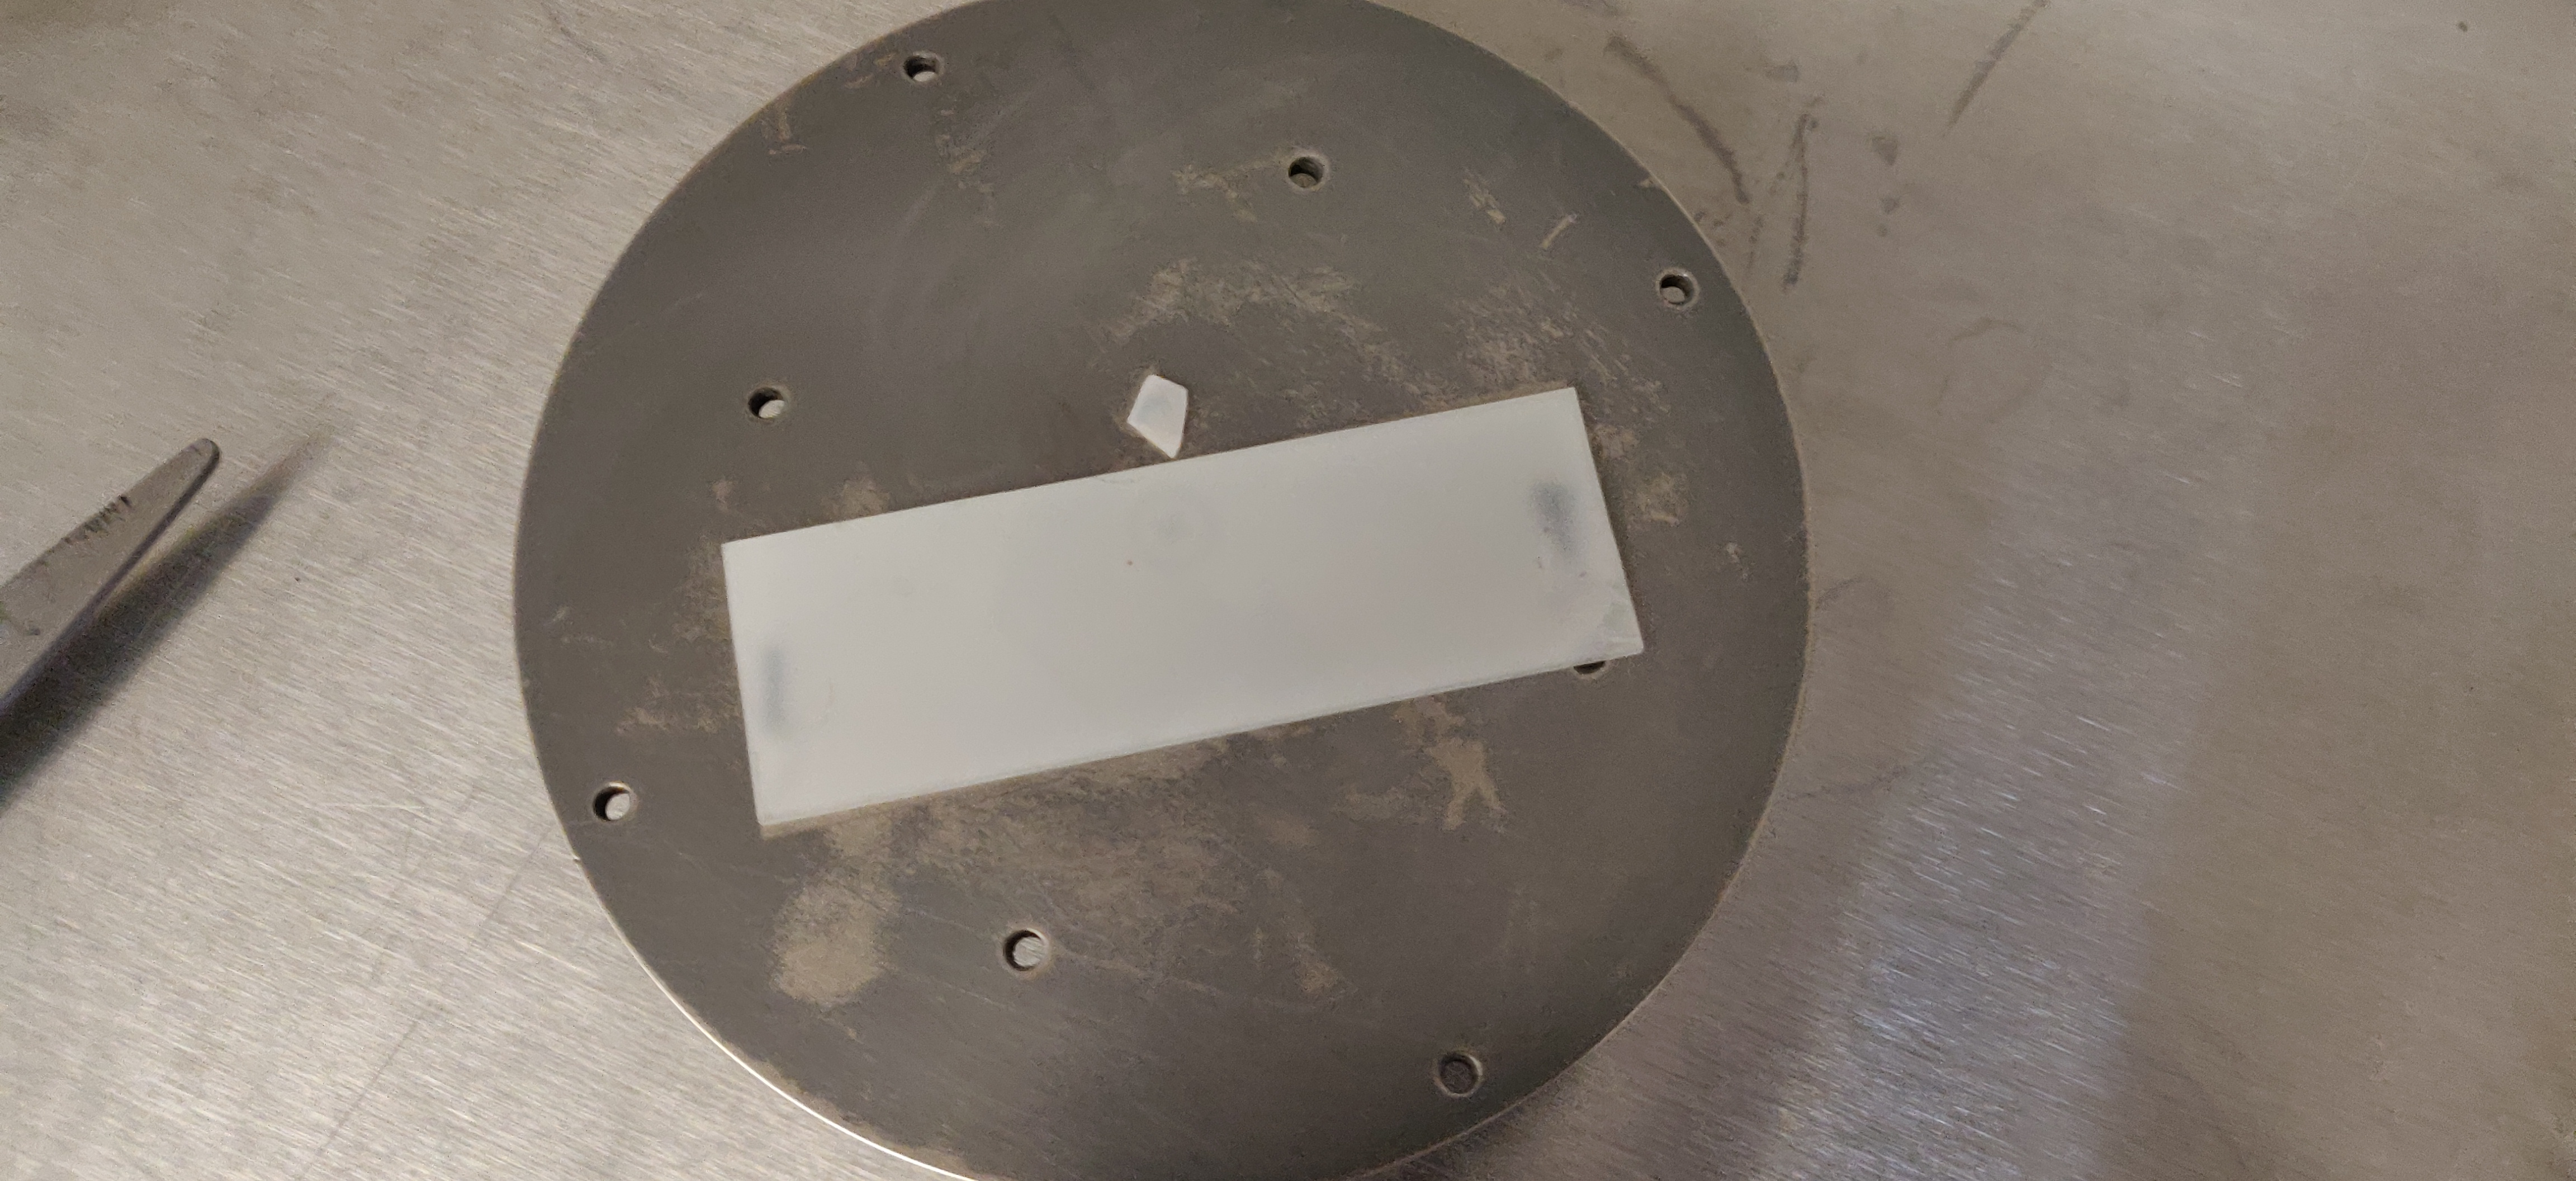
\includegraphics[width=.75\textwidth]{figs/4-Raman/slide-with-TeO2-film-on-substrate.jpeg}
  \hspace{1em}\caption{Glass slide with a \SI{1}{\micro\meter} thin film of \ce{TeO2} deposited via \ac{PVD} and subsequently annealed.}
  \label{fig:Raman:TeO2slide}
\end{figure}

\begin{figure}[h!]
  \centering
  \hspace{-2em}\includegraphics[width=.85\textwidth]{figs/4-Raman/CoBS Measurement: 1 μm TeO2 wide.png}
  \caption[Observed spectrum obtained through a \ac{CoBS} measurement of \SI{1}{\micro\meter} of \ce{TeO2}.]{Observed background-subtracted spectrum obtained through a \ac{CoBS} measurement of \SI{1}{\micro\meter} of \ce{TeO2} captured at maximum operating optical powers \(P_{\rm P}P_{\rm S}P_{\rm Pr} \approx \SI{0.25}{\cubic\watt}\), with 1\(\sigma\) uncertainties.}
  \label{fig:Raman:1umTeO2}
\end{figure}

To surmount this issue, we resolved to deposit \ce{Te} metal and apply a post-deposition annealing treatment to oxidize the \ce{Te} into the desired \ce{TeO2}. This fabrication procedure proved successful. Initial deposition rate stability issues were resolved by inserting custom electrical circuit logic into the deposition chamber voltage controls. The circuit logic provided added sensitivity of deposition parameters by introducing a switchable ``course'' and ``fine'' voltage control mode, with the fine setting containing the phenomenologically-found sweet-spot of resistance for thermally depositing \ce{Te} metal. In our experience, thermally depositing \si{\micro\meter} films of \ce{Te} metal via multiple successive deposition-annealing cycles of annealable sublayers, occuring over \(\sim\)\SI{20}{\hour}, and keeping the deposition rate steady with continuous adjustment of the fine-control knob is akin to rolling a ball lengthwise down the ouside of a pipe of diameter equal to the ball's. Nevertheless, this procedure proved a reliable method of producing \ce{TeO2} thin films deposited onto glass slides which could easily be inserted and secured in the beam path of the \ac{CoBS} instrument. Figure~\ref{fig:Raman:TeO2slide} shows an image of a glass slide with a deposited thin film of \ce{TeO2} which has been successfully annealed, converting the mirror-shine appearance of the deposited \ce{Te} into the semi-transparent appearance seen here. This sample is shown reattached to the \ac{PVD} substrate for additional layers to be deposited and subsequently annealed. The annealer was found to be capable of fully oxidizing a maximum of \(\sim\)\SI{300}{\nano\meter} of deposited \ce{Te}. This set the step size for building up \ce{TeO2} layers toward the total desired sample thickness.

\begin{figure}[th!]
  \centering
  \begin{subfigure}[b]{0.85\textwidth}
    \centering
    \hspace{-2em}\includegraphics[width=\textwidth]{figs/4-Raman/CoBS Measurement: 1 μm TeO2.png}
    \caption{Raw resolution.}
    \label{fig:Raman:1umTeO2Raw}
  \end{subfigure}

  \vspace{1em}

  \begin{subfigure}[b]{0.49\textwidth}
    \centering
    \includegraphics[width=\textwidth]{figs/4-Raman/CoBS Measurement: 1 μm TeO2 5 MHz bin.png}
    \caption{\SI{5}{\mega\hertz} binning.}
    \label{fig:Raman:1umTeO25MHzBin}
  \end{subfigure}
  \hfill
  \begin{subfigure}[b]{0.49\textwidth}
    \centering
    \includegraphics[width=\textwidth]{figs/4-Raman/CoBS Measurement: 1 μm TeO2 10 MHz bin.png}
    \caption{\SI{10}{\mega\hertz} binning.}
    \label{fig:Raman:1umTeO10MHzBin}
  \end{subfigure}

  \caption[Observed spectra obtained through a \ac{CoBS} measurement of \SI{1}{\micro\meter} of \ce{TeO2}.]{Observed background-subtracted spectra obtained through a \ac{CoBS} measurement of \SI{1}{\micro\meter} of \ce{TeO2} captured at maximum operating optical powers \(P_{\rm P}P_{\rm S}P_{\rm Pr} \approx \SI{0.25}{\cubic\watt}\), with 1\(\sigma\) uncertainties. Each panel shows the same data set under different binning resolutions.}
  \label{fig:Raman:1umTeO2_combined}
\end{figure}

\begin{figure}[t]
  \centering
  \hspace{-2em}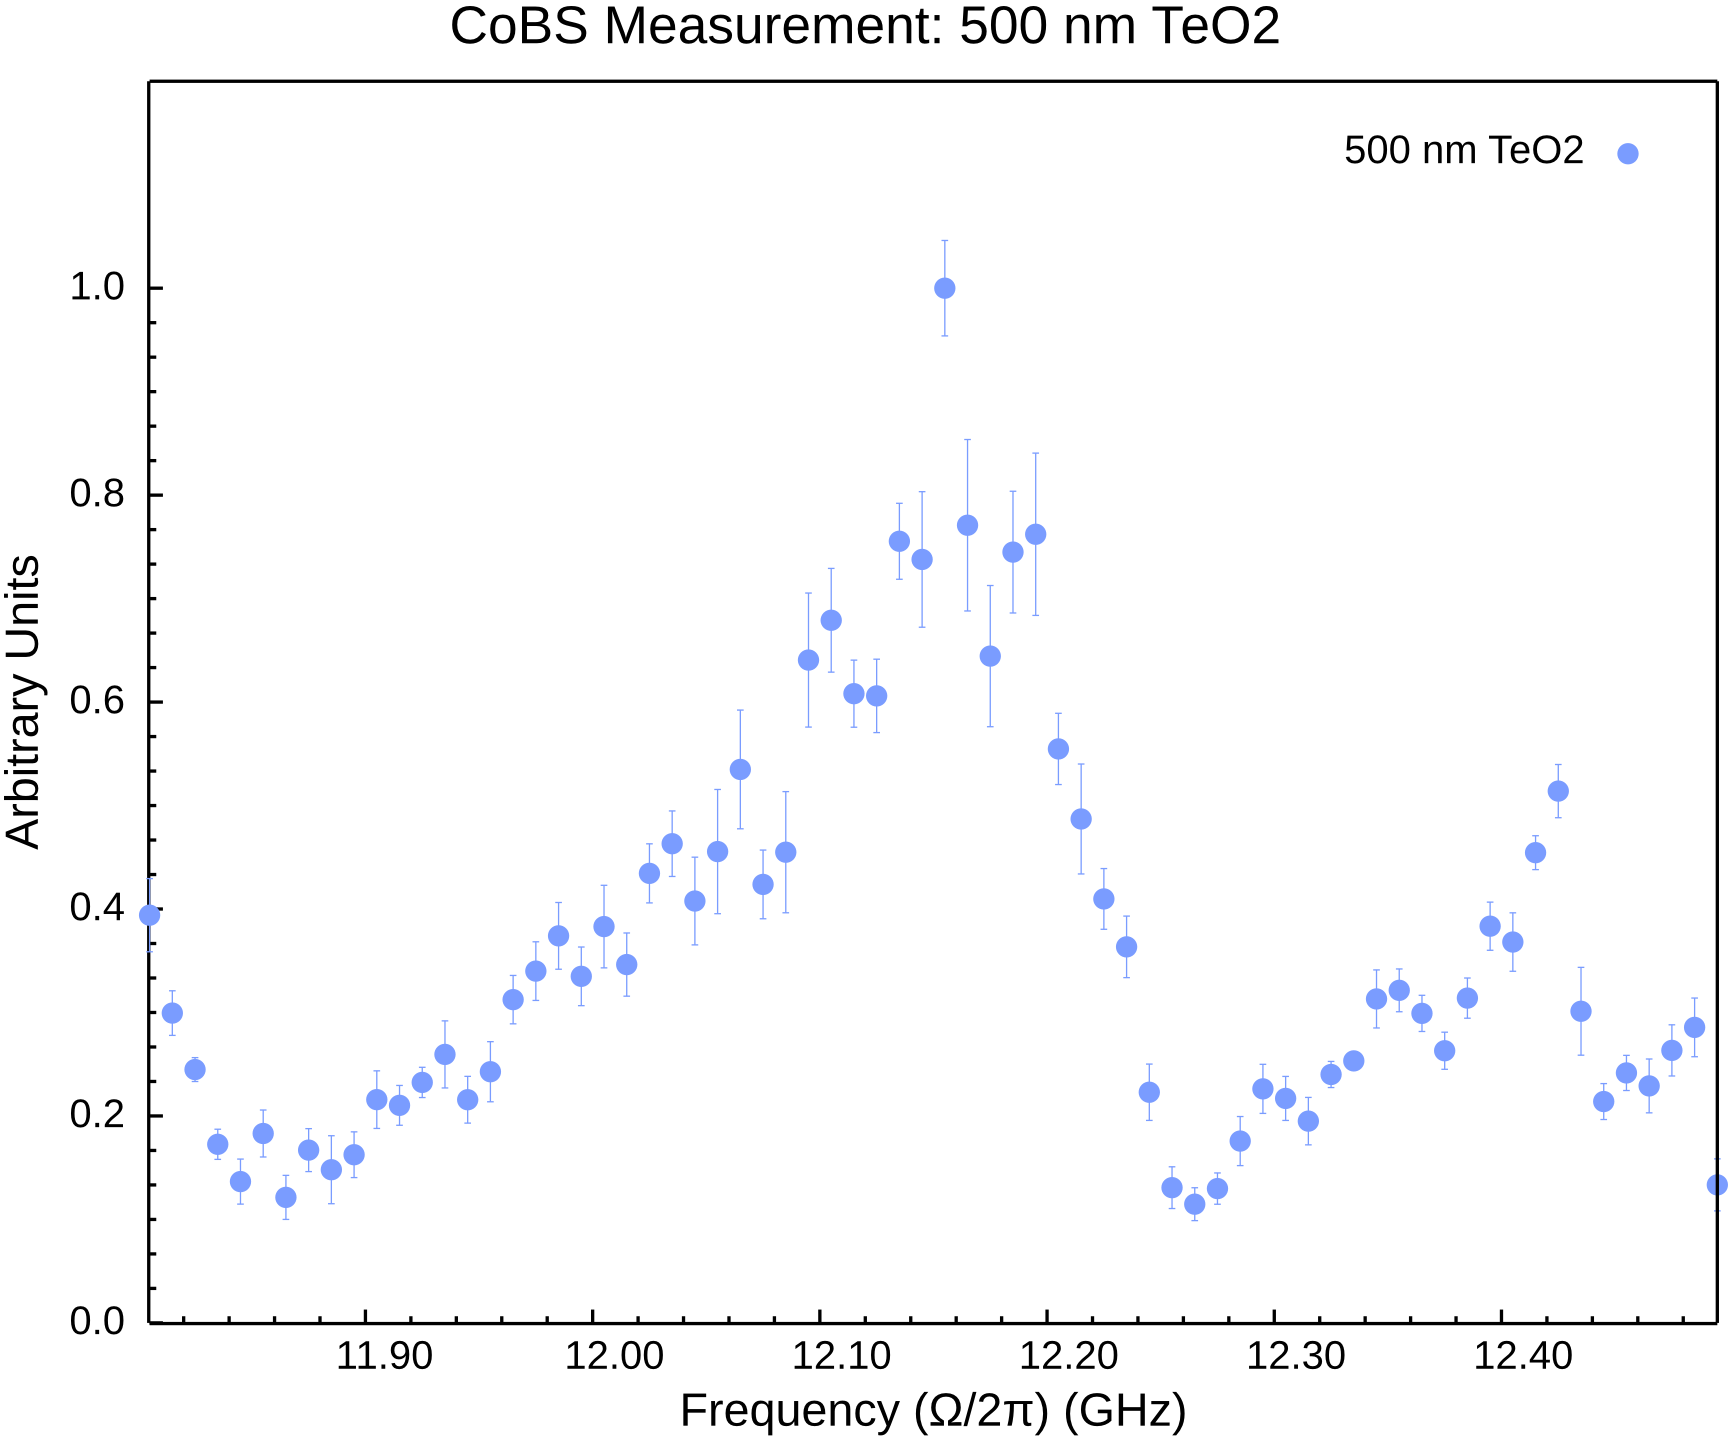
\includegraphics[width=.85\textwidth]{figs/4-Raman/CoBS Measurement: 500 nm TeO2.png}
  \caption[Observed spectrum obtained through a \ac{CoBS} measurement of \SI{500}{\nano\meter} of \ce{TeO2}.]{Observed background-subtracted spectrum obtained through a \ac{CoBS} measurement of \SI{500}{\nano\meter} of \ce{TeO2} captured at maximum operating optical powers \(P_{\rm P}P_{\rm S}P_{\rm Pr} \approx \SI{0.25}{\cubic\watt}\), with 1\(\sigma\) uncertainties.}
  \label{fig:Raman:500nmTeO2}
\end{figure}

Figure~\ref{fig:Raman:1umTeO2} shows a \ac{CoBS} measurement of a \SI{1}{\micro\meter} thin film of \ce{TeO2}. From reported sound speed and refractive index for \ce{TeO2}, \cite{uchida1969elastic, schweppe1970elastic, ohmachi1972acoustic, peercy1975temperature, fleury2018non, harris1991multichannel, uchida1971optical} Equation~\ref{eq:Raman:f_B} predicts a Brillouin frequency shift for \ce{TeO2} to be \(f_{\rm B}\approx\SI{12.4(0.5)}{\giga\hertz}\). An independent measurement was performed on a second \SI{1}{\micro\meter} thin film of \ce{TeO2} prepared in the same way. For this second measurement, after capturing the \ce{TeO2} film spectra, a repeated measurement was immediately performed in which the \ce{TeO2} sample was removed and a measurement was taken under identical parameters. Figure~\ref{fig:Raman:1umTeO2_combined} shows the result of these two measurements in three variations in resolution via binning: unbinned raw resolution (Figure~\ref{fig:Raman:1umTeO2Raw}), \SI{5}{\mega\hertz} bins (Figure~\ref{fig:Raman:1umTeO25MHzBin}), and \SI{10}{\mega\hertz} bins (Figure~\ref{fig:Raman:1umTeO10MHzBin}). While perfectly crystalline \ce{TeO2} features a smaller linewidth \(\sim\)\SI{10}{\mega\hertz}, \cite{renninger2018bulk} dissipation within a rough amorphous thin film of varying grain size and imperfect crystal structure would feature significantly higher dissipation (wider linewidth) than its crystalline counterpart. These same imperfections would contribute to a slighly slower sound speed in the deposited \ce{TeO2}, pushing the Brillouin frequency shift slightly higher (see Equation~\ref{eq:Raman:f_B}). As previously noted, a measurement of \SI{1}{\micro\meter} \ce{TeO2} would require at least as great as \(\sim\)\SI{76}{\femto\watt}, which is within of the capability of the demonstrated \(\sim\)\SI{5}{\femto\watt} sensitivity of our \ac{CoBS} instrument. Further measurements are required to confirm a measurement of a \SI{1}{\micro\meter} deposited thin film of \ce{TeO2} with the \ac{CoBS} instrument.

Figure~\ref{fig:Raman:500nmTeO2} shows a spectrum obtained for a \SI{500}{\nano\meter} thin film of \ce{TeO2}. A pronounced background noise profile dominates the spectrum, with no significant spectral features indicative of a measurement of \ce{TeO2}. While the scattered power produced from \SI{500}{\nano\meter} of \ce{TeO2} (\(P_{\rm CoBS,\,\SI{500}{\nano\meter}\,\ce{TeO2}} \approx \SI{19}{\femto\watt}\)) remains just within the sensitivity limit of the instrument, in practice, a host of non-ideal experimental conditions could prevent the instrument from performing at its full sensitivity limit. In search of other options, and having worked extensively with \ce{Te} metal over so many hours of \ac{PVD} depostions, we began researching the possibility of using un-annealed \ce{Te} over its oxidized counterpart due to the meanwhile discovered tremendously higher material gain factor offered by \ce{Te} the metal over its oxidized state \ce{TeO2}.

\subsection{\texorpdfstring{\ce{Te}}{Te} Thin Film}
\label{subsec:Raman:Target:Te}

Table~\ref{tab:Raman:Te} gives the relevant parameters for \ce{Te} metal. While \ce{Te} is absorptive at \SI{1.55}{\micro\meter}, transmission becomes meaningful as films become thinner, with a \SI{1}{\micro\meter} thin film of \ce{Te} permitting 11.4\% of \SI{1.55}{\micro\meter} light to transmit and a \SI{500}{\nano\meter} film permitting 29\%. \cite{ciesielski2018permittivity} The \(n = 4.58\) refractive index of \ce{Te} contributes to a massive material Brillouin gain of \(g_{0} = \SI{13.1}{\meter\per\giga\watt}\), translating to an acousto-optic overlap-adjusted effective Brillouin gain \(G_{\rm B} = \SI{14.4}{\per\meter\per\watt}\) (see Figure~\ref{fig:Raman:GainofRelevantMaterials}). With no successful measurements for \ce{TeO2} thin films achieved, this much higher gain of \ce{Te} presented an enticing opportunity.

\begin{table}[t]
    \centering
    \begin{tabular}{c c c c c c c c c}
        \toprule
        \textbf{\ce{Te}} &
        \(\mathbf{\Gamma_{\rm \textbf{B}}}^{\rm a}\) &
        \(\mathbf{\tau}\) &
        \(\mathbf{v_{\rm \textbf{s,\,long}}}^{\rm b}\) &
        \(\mathbf{n}^{\rm c}\) &
        \(\mathbf{L_{\rm \textbf{coh}}}\) &
        \(\mathbf{P_{\rm \textbf{CoBS,\,500\,nm}}}\) &
        \(\mathbf{\Omega_{\rm \textbf{B}}}\) &
        \(\mathbf{\Omega_{\rm \textbf{R,\,1\,\(\boldsymbol{\mu}\)m}}}\) \\
        &
        (\si{\mega\hertz}) &
        (\si{\nano\second}) &
        (\si{\meter\per\second}) &
        &
        (\si{\micro\meter}) &
        (\si{\pico\watt}) &
        (\si{\giga\hertz}) &
        (\si{\giga\hertz}) \\
        \midrule
        \\
        \textbf{Bulk} & \(\sim2\pi\cdot\)\num{10} & \num{100} & \(\sim\)\num{2610} & \num{4.58} & \num{261} & \(\sim\)\num{80e-3} & \(2\pi\cdot\)\num{15.4} & \(2\pi\cdot\)\num{1.31} \\
        \\
        \bottomrule
        \\
        \multicolumn{9}{l}{
        a: \citenum{balakshii2008investigation, lin2016tellurium, voloshinov2017optic, khorkin2020acousto, voloshinov2008acousto},
        b: \citenum{balakshii2008investigation, lin2016tellurium, voloshinov2017optic, khorkin2020acousto, voloshinov2008acousto, kozhevnikov2007sound},
        c: \citenum{ciesielski2018permittivity, hartig1954infrared}
        } \\
    \end{tabular}
    \caption[Material parameters for \ce{Te} relevant to observing Brillouin traveling-wave modes and Raman standing-wave modes.]{Material parameters for \ce{Te} relevant to observing Brillouin traveling-wave modes and Raman standing-wave modes, obtained from published values for bulk \ce{Te} as well as for \ce{Te} thin films. Here, \(\Gamma_{\rm B}\) is the angular Brillouin linewidth (phonon dissipation rate) and the inverse of phonon lifetime \(\tau = 2\pi\Gamma_{\rm B}^{-1}\), \(v_{\rm s,\,long}\) is the longitudinal sound speed, \(n\) is the refractive index, \(l_{\rm coh}\) is the phonon coherence length (mean travel distance), and \(P_{\rm CoBS}\) is the scattered power for the \ac{CoBS} process, reported here for \SI{500}{\nano\meter} \ce{Te}, and scales with \(L^{2}\) (Equation~\ref{eq:Raman:ScatteredPowerPhi}). Finally, \(\Omega_{\rm B}\) is the angular Brillouin frequency shift (Equation~\ref{eq:Raman:f_B}), and \(\Omega_{\rm R,\,\SI{1}{\micro\meter}}\) is the first harmonic (\(n=1\)) of the fundamental \(L_{0}\) Raman-like mode for \(L=\) \SI{1}{\micro\meter} (Equation~\ref{eq:Raman:f_R}). While \ce{CS2} and \ce{TeO2} are transparent at \SI{1.55}{\micro\meter}, \ce{Te} is absorptive here. However, transmission becomes meaningful through thin films, with \SI{1}{\micro\meter} of deposited \ce{Te} permitting 11.4\% and \SI{500}{\nano\meter} permitting 29\% of \SI{1.55}{\micro\meter} light to transmit. \cite{ciesielski2018permittivity} This extra \(\sim\)70\% loss (for each of the three optical fields) has been accounted for in the scattered power value for the \ac{CoBS} process listed in the table.}
    \label{tab:Raman:Te}
\end{table}

\begin{figure}[t]
  \centering
  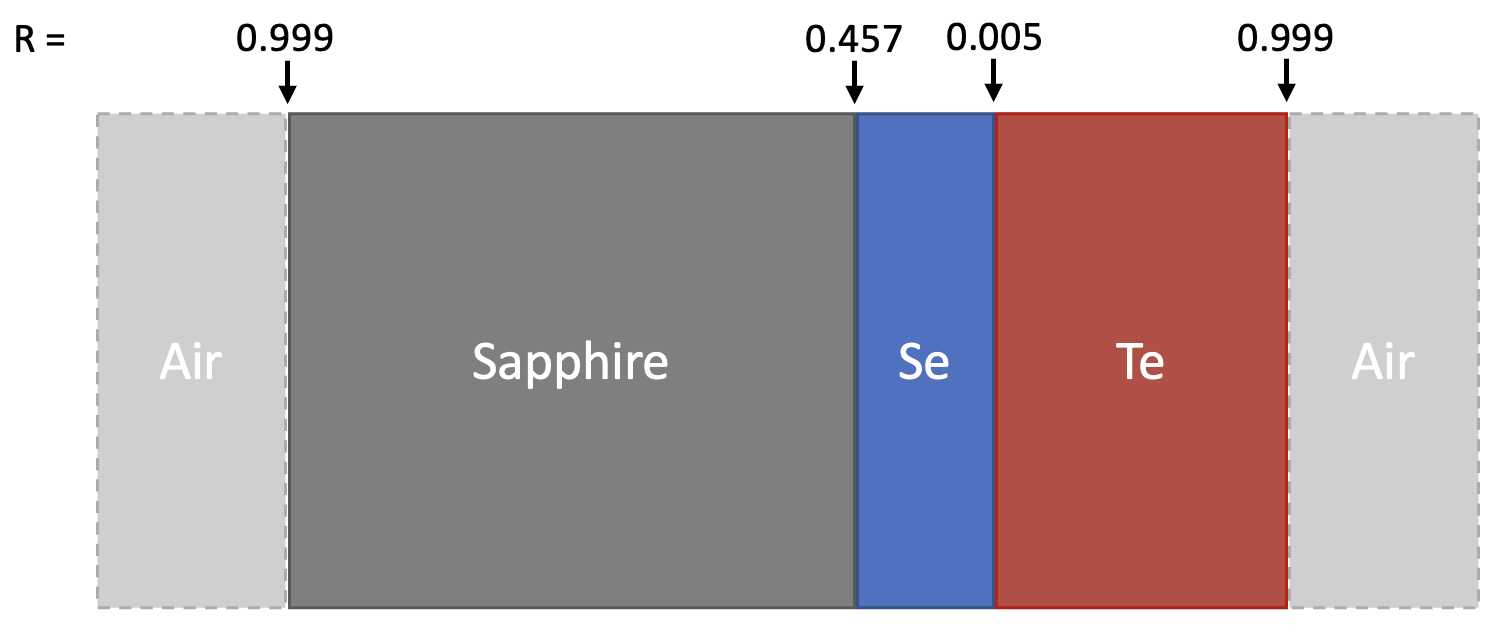
\includegraphics[width=.8\textwidth]{figs/4-Raman/AcousticImpedance.png}
  \caption[Illustration of the material layers of a \ce{Te} thin film sample.]{Illustration of the material layers of a \ce{Te} thin film sample. Sapphire (\ce{Al2O3}) substrates are primed with a \SI{10}{\nano\meter} deposited layer of \ce{Se} by collaborators Dr. Alessandro Mazza of \acl{LANL} (\ac{LANL}) and the \acl{CINT} (\ac{CINT}) and Dr. Matthew Brahlek of \acl{ORNL} (\ac{ORNL}). This \ce{Se} layer acts as an adhesion layer between the sapphire and the \ce{Te} film. Acoustic reflectivity values at each interface as a result of the acoustic impedance mismach between materials are shown along the top of the illustration for each material boundary.}
  \label{fig:Raman:AcousticImpedance}
\end{figure}

\begin{figure}[h!]
  \centering
  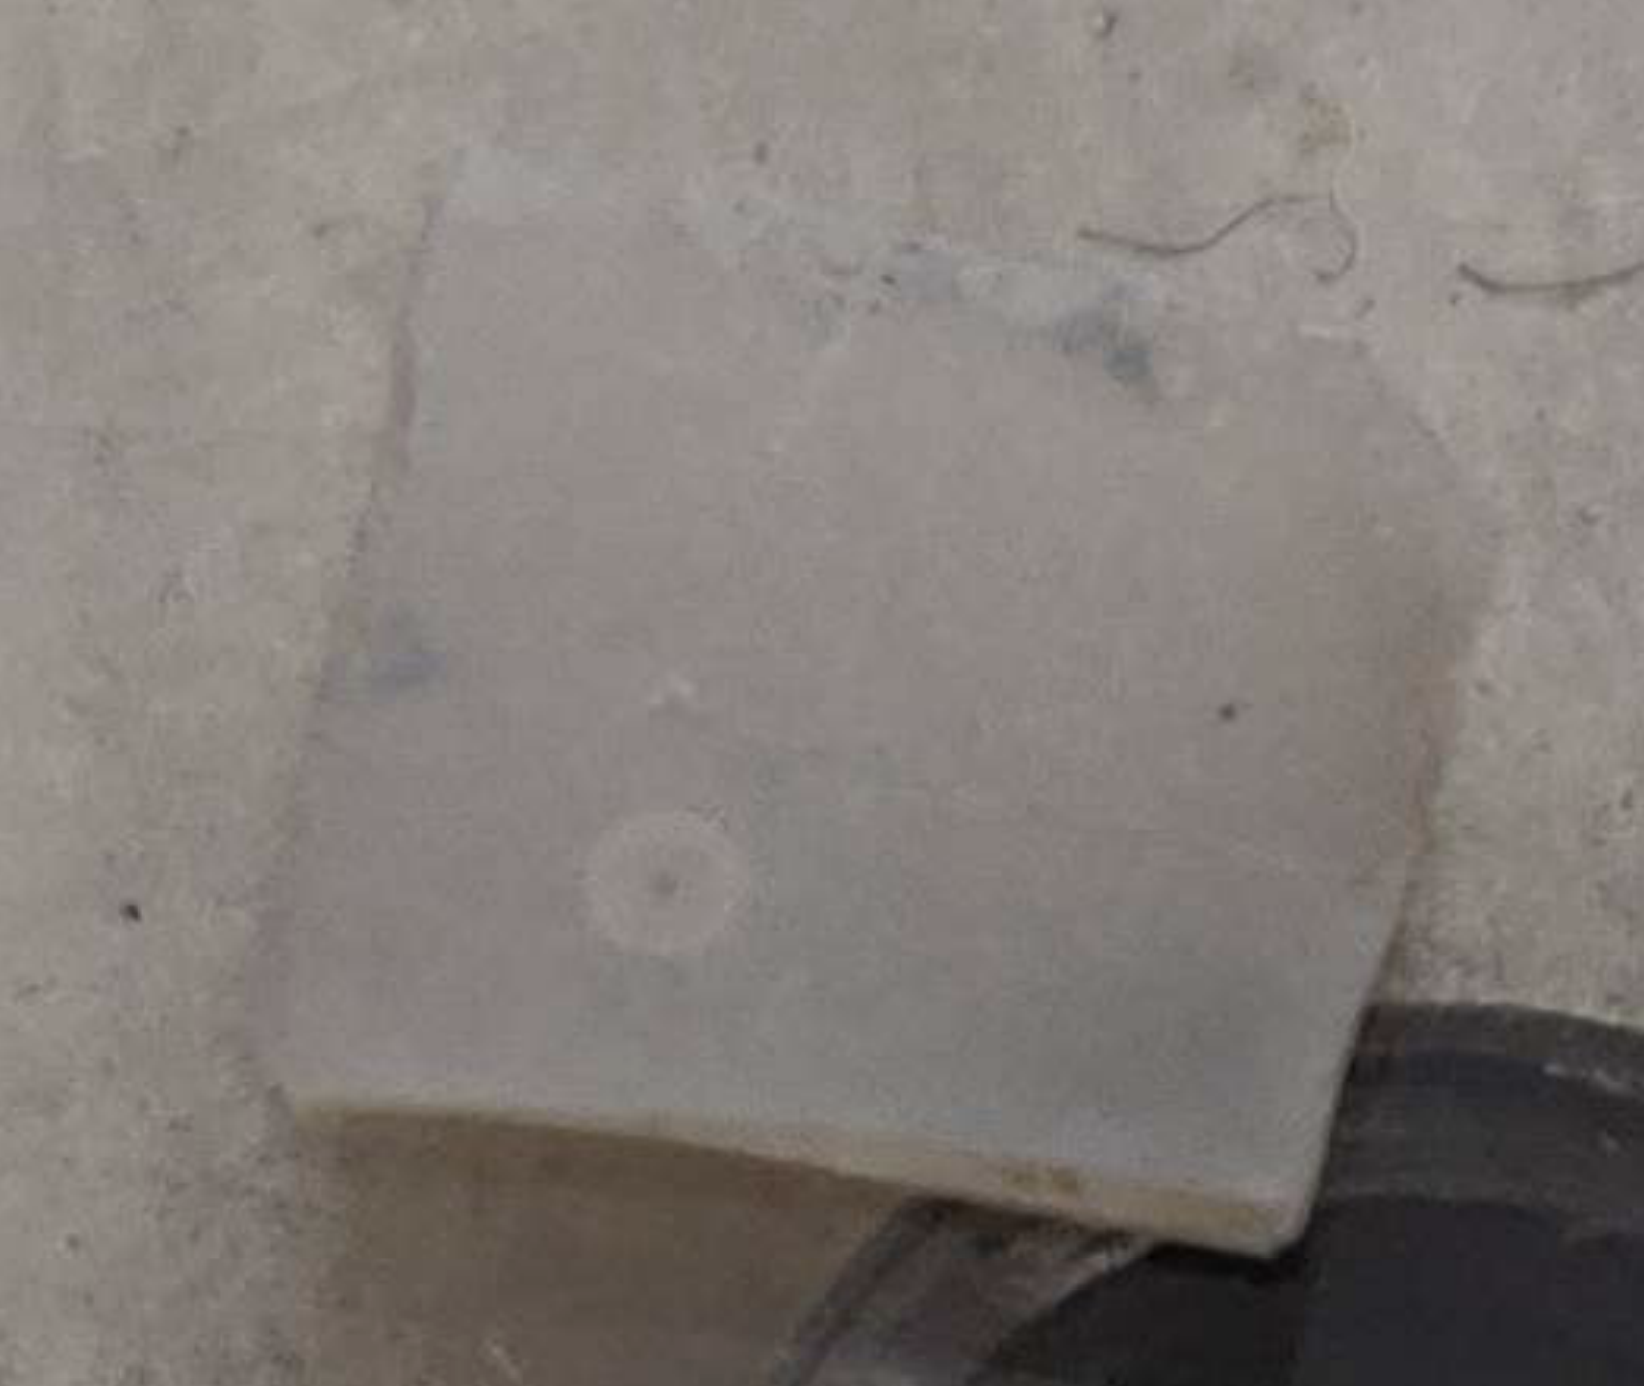
\includegraphics[width=.3\textwidth]{figs/4-Raman/TeTeO2beamspot.png}
  \caption[Evidence of oxidization of the \SI{500}{\nano\meter} \ce{Te} thin film in the circular beam spot.]{Evidence of oxidization of the \SI{500}{\nano\meter} \ce{Te} thin film in the circular beam spot due to \(\sim\)70\% absorption of the \SI{1.55}{\micro\meter} optical fields.}
  \label{fig:Raman:TeTeO2beamspot}
\end{figure}

Initial \ac{CoBS} measurements of \ce{Te} thin films resulted in evident ablation of the film from the glass substrate, with poor adhesion between the \ce{Te} and glass slide the determined cause. Collaborators at the \acl{CINT} (\ac{CINT}), a joint center affiliated with \ac{LANL} and \ac{SNL}, lent the insight that a thin adhesion layer of \ce{Se} is recommended between \ce{Te} deposited onto glass. \ce{Se}-primed sapphire substrate samples were kindly prepared and sent to us by Dr. Alessandro Mazza of \ac{LANL} and Dr. Matthew Brahlek of \ac{ORNL}, ready for depositions of \ce{Te} to be performed ontop of a \SI{10}{\nano\meter} \ce{Se} layer. The \ce{Se} adhesion layer proved successful in adhering the \ce{Te}. A diagram of the material layering is shown in Figure~\ref{fig:Raman:AcousticImpedance}. A \SI{500}{\nano\meter} thin film of \ce{Te} was fabricated after estimations of a feasible measurement of the material showed a required sensitivity \(\sim\)\(15\times\) the sensitivity limit of the instrument. During measurement, it was discovered that the energy of the optical powers incident on the sample (of which \(\sim\)71\% is absorbed as previously discussed) caused significant heating in the thin film of \ce{Te}, resulting in oxidization of the \ce{Te}, changing its state into \ce{TeO2} within the beam spot. Figure~\ref{fig:Raman:TeTeO2beamspot} shows a photograph which captures this resulting oxidized state of the \ce{Te} thin film after sitting for a measurement in the beam path of the instrument.

With this result, we began a broader reanalysis of the choice of platform for observing Brillouin-induced Raman modes at room temperature. Figure~\ref{fig:Raman:AcousticImpedance} also shows acoustic reflectivity values \(R\) for each interface of a \ce{Te} sample, calculated by Equations~\ref{eq:Raman:acoustic reflectivity} and \ref{eq:Raman:acoustic impedance}. While the \ce{Te}-air boundary offers near complete acoustic reflection, owing to the large acoustic impedance mismatch between \ce{Te} and air, the acoustic reflectivity is near zero between \ce{Te} and \ce{Se} and only \(\sim\)50% between the \ce{Se} and the sapphire substrate. These values are similar for \ce{TeO2} in place of \ce{Te}. To ultimately observe Raman modes, there must be sufficient confinement of the phonons. After some consideration of dissolvable substrates which may be engineered to expose a portion of the \ce{Te} or \ce{TeO2} to air on both sides, recovering both free bounds, we returned to the last confirmed successfully measured material: \ce{CS2}.

\subsection{\texorpdfstring{\ce{CS2}}{CS2} Micrometer Cell}
\label{subsec:Raman:Target:CS2Cells}

\begin{table}[t]
  \centering
  \begin{tabular}{c c c c c c c c c}
    \toprule
    \textbf{\ce{CS2}} &
    \(\mathbf{\Gamma_{\rm \textbf{B}}}^{\rm a}\) &
    \(\mathbf{\tau}\) &
    \(\mathbf{v_{\rm \textbf{s,\,long}}}^{\rm b}\) &
    \(\mathbf{n}^{\rm c}\) &
    \(\mathbf{L_{\rm \textbf{coh}}}\) &
    \(\mathbf{P}_{\mathbf{CoBS,\,\boldsymbol{L}_{\mathbf{coh}}/2}}\) &
    \(\mathbf{\Omega_{\rm \textbf{B}}}\) &
    \(\mathbf{\Omega}_{\mathbf{R,\,1\,\boldsymbol{\micro}m}}\) \\
    &
    (\si{\mega\hertz}) &
    (\si{\nano\second}) &
    (\si{\meter\per\second}) &
    &
    (\si{\micro\meter}) &
    (\si{\pico\watt}) &
    (\si{\giga\hertz}) &
    (\si{\giga\hertz}) \\
    \midrule
    \\
    \textbf{Liquid} & \(2\pi\cdot\)\num{90(10)} & \num{10} & \num{1150} & \num{1.59} & \num{13(2)} & \(\sim\)\num{7.2} & \(2\pi\cdot\)\num{2.54(3)} & \(2\pi\cdot\)\num{0.575} \\
    \\
    \bottomrule
    \\
    \multicolumn{9}{l}{
      a: \citenum{boyd2020nonlinear, johnson2023laser, enright1974depolarized, coakley1975brillouin},
      b: \citenum{boyd2020nonlinear, johnson2023laser, behunin2019spontaneous, geilen2023extreme},
      c: \citenum{boyd2020nonlinear, johnson2023laser}
    } \\
  \end{tabular}
  \caption[Material parameters for bulk liquid \ce{CS2} relevant to observing Brillouin traveling-wave modes and Raman standing-wave modes.]{Material parameters for bulk liquid \ce{CS2} relevant to observing Brillouin traveling-wave modes and Raman standing-wave modes, obtained from published values as well as our own observations shown in Figures~\ref{fig:Raman:1cmCS2}, \ref{fig:Raman:4mmCS2}, \ref{fig:Raman:1mmCS2}, and \ref{fig:Raman:100umCS2}. Here, \(\Gamma_{\rm B}\) is the angular Brillouin linewidth (phonon dissipation rate) and the inverse of phonon lifetime \(\tau = 2\pi\Gamma_{\rm B}^{-1}\), \(v_{\rm s,\,long}\) is the longitudinal sound speed, \(n\) is the refractive index, \(l_{\rm coh}\) is the phonon coherence length (mean travel distance), and \(P_{\rm CoBS}\) is the scattered power for the \ac{CoBS} process, reported here for \(L_{\rm coh} = 2 \cdot \SI{6.5}{\micro\meter}\) \ce{CS2}, and scales with \(L^{2}\) (Equation~\ref{eq:Raman:ScatteredPowerPhi}). Finally, \(\Omega_{\rm B}\) is the angular Brillouin frequency shift (Equation~\ref{eq:Raman:f_B}), and \(\Omega_{\rm R,\,\SI{10}{\micro\meter}}\) is the first harmonic (\(n=1\)) of the fundamental \(L_{0}\) Raman-like mode for \(L=\) \SI{1}{\micro\meter} (Equation~\ref{eq:Raman:f_R}).}
  \label{tab:Raman:CS2}
\end{table}

Table~\ref{tab:Raman:CS2} gives the relevant material parameters for achieving Brillouin-induced Raman modes in \ce{CS2}. Notably, the phonon dissipation rate within \ce{CS2} is nearly \(10\times\) greater than that of \ce{TeO2} or \ce{Te}, at \(\Gamma_{\rm B} = \SI{90(10)}{\mega\hertz}\). This, in combination with its slower speed of sound \(V_{\rm s} = \SI{1150}{\meter\per\second}\), results in a short phonon coherence length \(L_{\rm coh} = \SI{13(2)}{\micro\meter}\) and a correspondingly high sensitivity requirement of \(P_{\rm CoBS,\,\SI{6.5}{\micro\meter}} \approx \SI{7.2}{\pico\watt}\). While this is smaller than the half-coherent-length sensitivity requrired for \ce{TeO2} (\SI{6.5}{\micro\meter} vs \SI{41.5}{\micro\meter} for \ce{TeO2}), making for a harder measurement to observe Raman modes in \ce{CS2} than \ce{TeO2} by this metric, the reduced complexity of the \ce{CS2} experimental platform as compared to the amorphous thin films presented as attractive. Additionally, the air-\ce{CS2}-air boundaries represent near total acoustic confinement at the interfaces, and the narrower Raman mode spacing (multiples of \(f_{\rm R,\,\ce{CS2}} = \SI{575}{\mega\hertz}\), as opposed to \(f_{\rm R,\,\ce{TeO2}} = \SI{2.13}{\giga\hertz}\)) in combination with the wider linewidth of \ce{CS2} together offered the possibility of more achievable length-tuning for Raman mode placement near the Brillouin frequency shift.

\begin{figure}[t]
    \centering
    \begin{subfigure}[b]{0.3\textwidth}
        \centering
        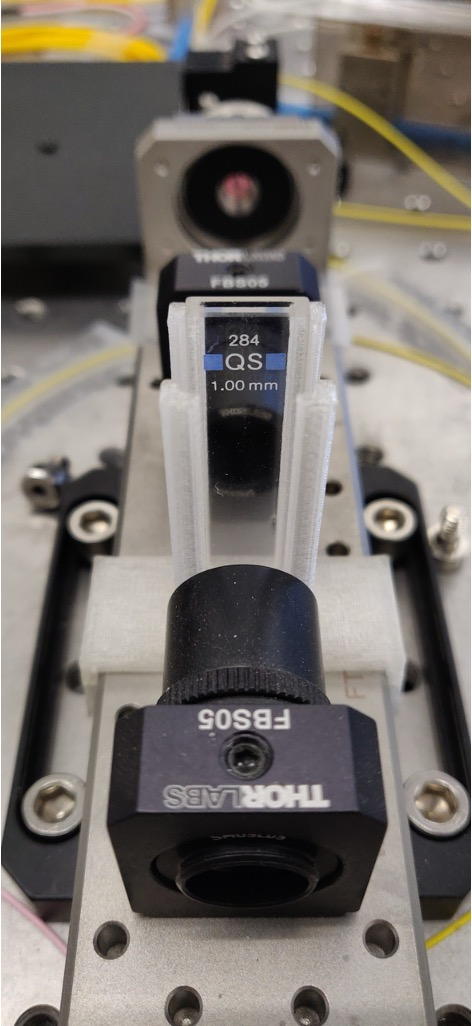
\includegraphics[width=\textwidth]{figs/4-Raman/1mmCS2.jpg}
        \caption{}
        \label{fig:Raman:1mmCS2pic}
    \end{subfigure}
    \hfill
    \begin{subfigure}[b]{0.3\textwidth}
        \centering
        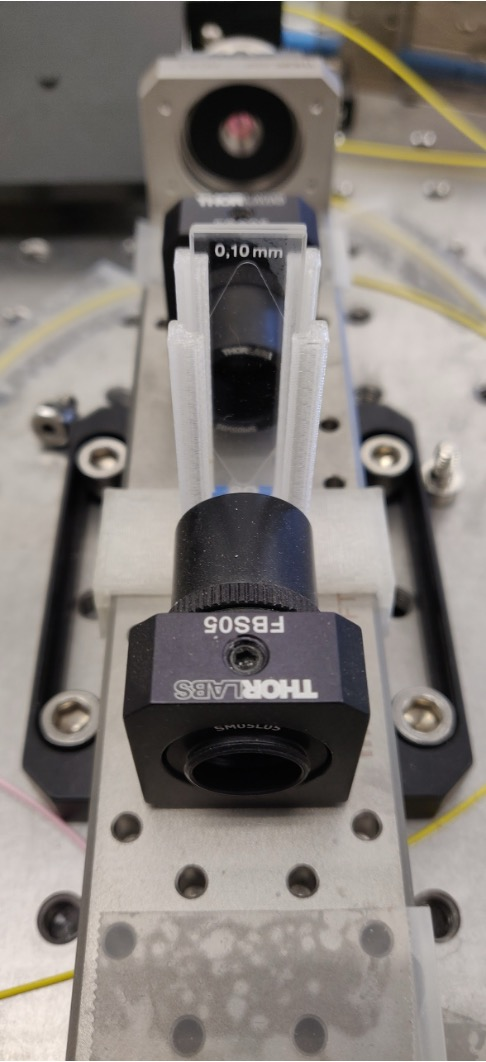
\includegraphics[width=\textwidth]{figs/4-Raman/100umCS2.jpg}
        \caption{}
        \label{fig:Raman:100umCS2pic}
    \end{subfigure}
    \hfill
    \begin{subfigure}[b]{0.3\textwidth}
        \centering
        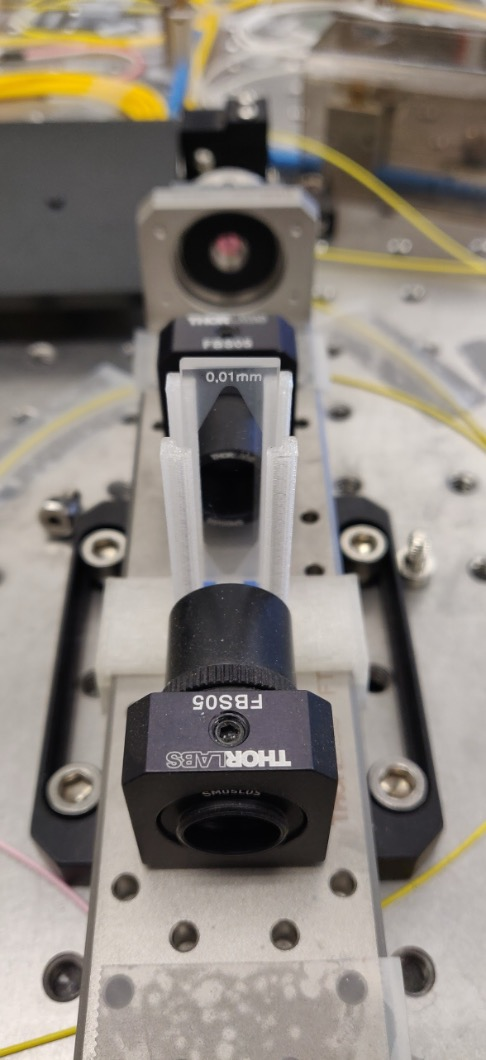
\includegraphics[width=\textwidth]{figs/4-Raman/10umCS2.jpg}
        \caption{}
        \label{fig:Raman:10umCS2pic}
    \end{subfigure}
    %
    \caption{Three \ce{CS2} cells of different path lengths (\SI{1}{\milli\meter}, \SI{100}{\micro\meter}, and \SI{10}{\micro\meter}) secured in the beam path of the \acl{CoBS}.}
    \label{fig:Raman:CS2cellpics}
\end{figure}

\begin{figure}[h!]
  \centering
  \begin{subfigure}[b]{0.48\textwidth}
    \centering
    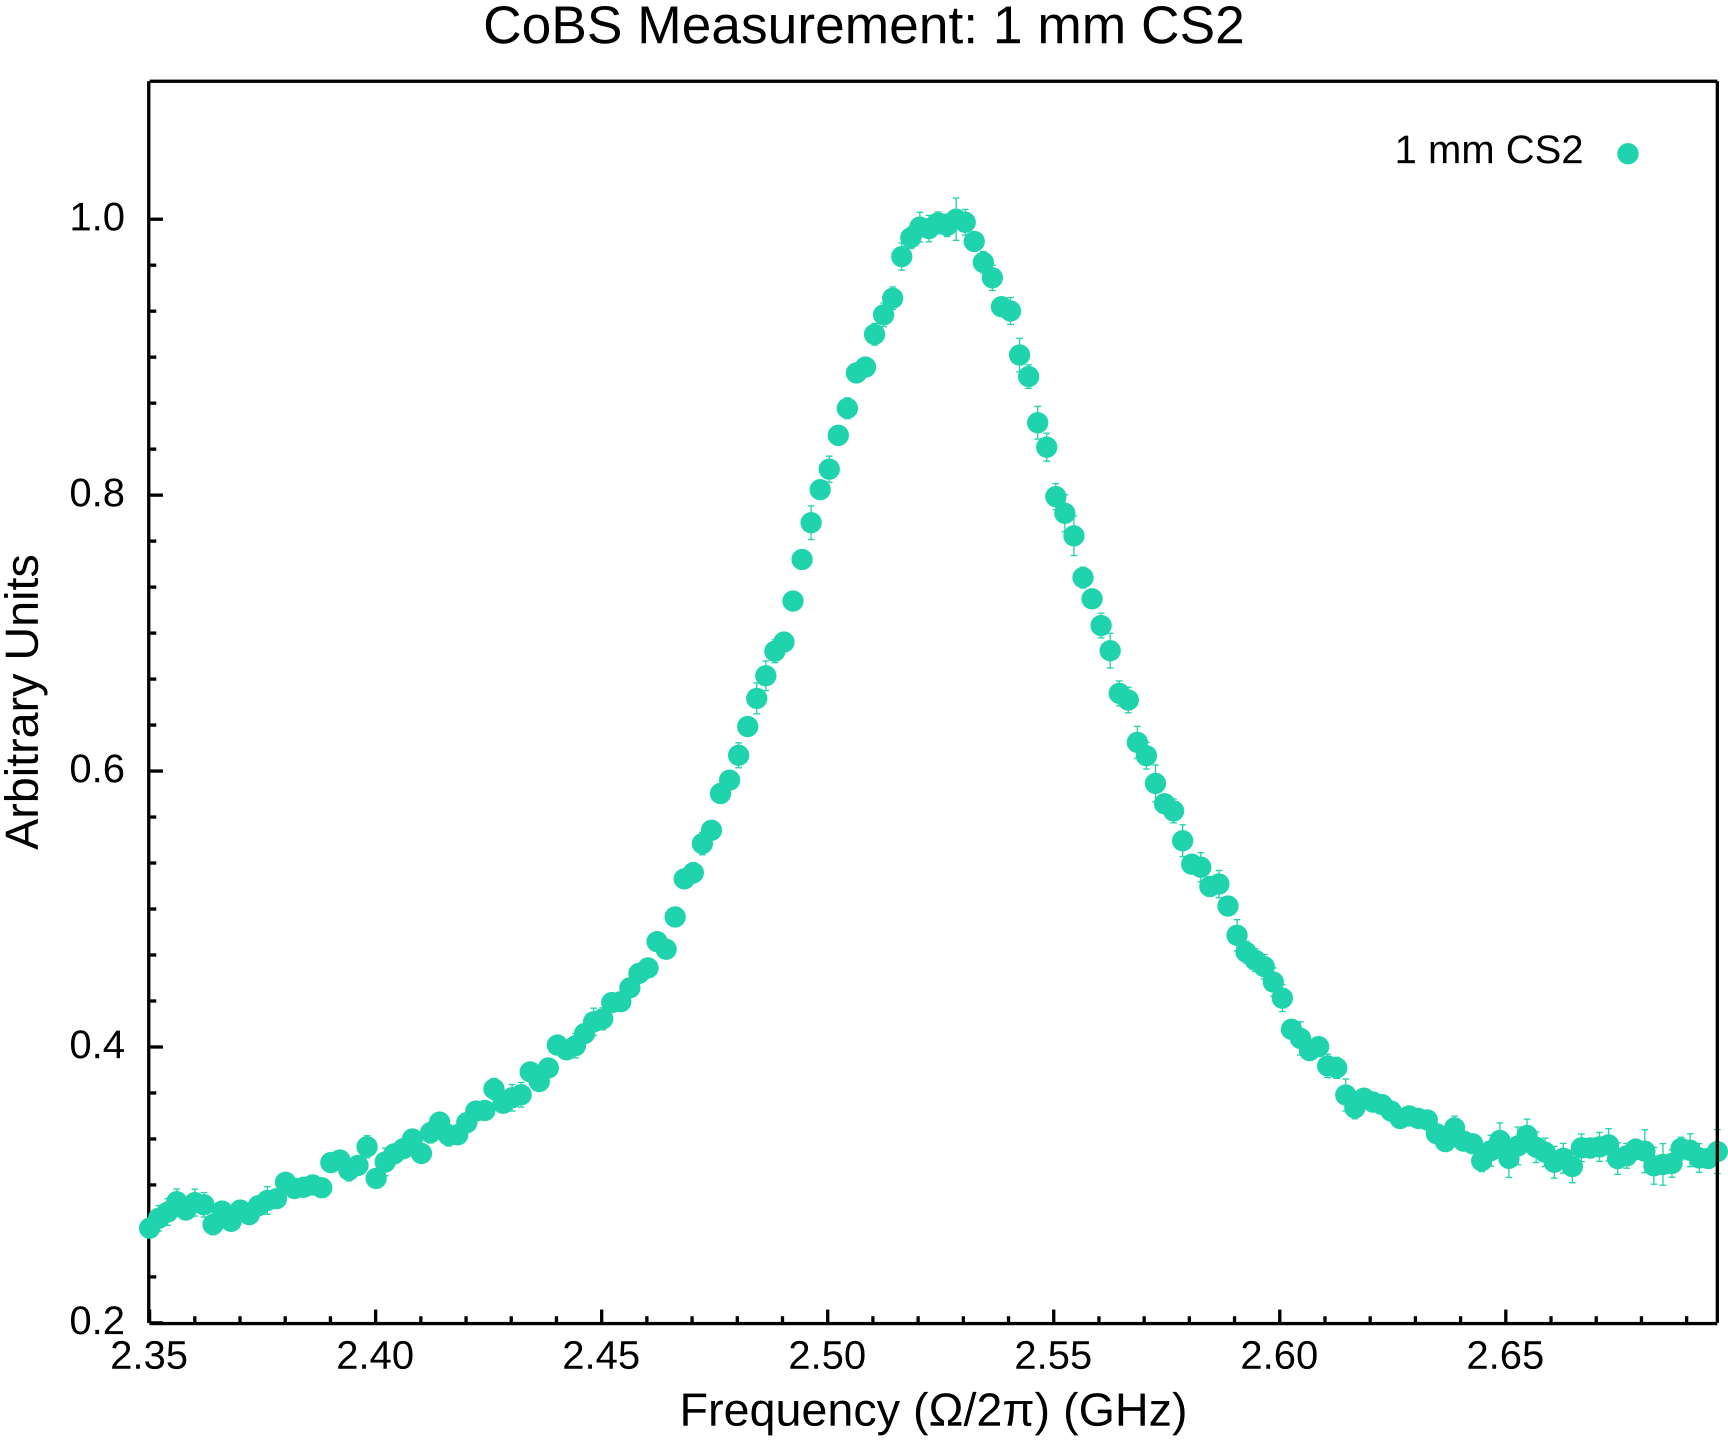
\includegraphics[width=\textwidth]{figs/4-Raman/CoBS Measurement: 1 mm CS2.png}
    \caption{}
    \label{fig:Raman:1mmCS2}
  \end{subfigure}
  \hfill
  \begin{subfigure}[b]{0.48\textwidth}
    \centering
    \includegraphics[width=\textwidth]{figs/4-Raman/CoBS Measurement: 100 μm CS2.png}
    \caption{}
    \label{fig:Raman:100umCS2}
  \end{subfigure}
  \vspace{1em}
  \begin{subfigure}[b]{0.48\textwidth}
    \centering
    \includegraphics[width=\textwidth]{figs/4-Raman/CoBS Measurement: 10 μm CS2.png}
    \caption{}
    \label{fig:Raman:10umCS2}
  \end{subfigure}
  \caption[Observed spectra obtained through a \acs{CoBS} measurement of \SI{1}{\milli\meter}, \SI{100}{\micro\meter}, and \SI{10}{\micro\meter} liquid \ce{CS2}.]{Observed background-subtracted spectra obtained through \ac{CoBS} measurements of \textbf{(a)} \SI{1}{\milli\meter}, \textbf{(b)} \SI{100}{\micro\meter}, and \textbf{(c)} \SI{10}{\micro\meter} liquid \ce{CS2} (pictured in Figure~\ref{fig:Raman:10umCS2}), captured at maximum operating optical powers \(P_{\rm P}P_{\rm S}P_{\rm Pr} \approx \SI{0.25}{\cubic\watt}\). All measurements have 1\(\sigma\) uncertainties smaller than the data point markers.}
  \label{fig:Raman:CS2combined}
\end{figure}

Small path length cells were obtained for \SI{1}{\milli\meter}, \SI{100}{\micro\meter}, and \SI{10}{\micro\meter} path lengths. Figure~\ref{fig:Raman:CS2cellpics} show photographs of each of these cells inserted into the sample holder and installed into the sample stage of \ac{CoBS}. Progressive measurements were attempted, with each 10\(\times\) decrease in effective length \(L\) corresponding to a 100\(\times\) decrease in scattered power produced, and thereby a 100\(\times\) higher sensitivity required for a successful measurement (see Equation~\ref{eq:Raman:ScatteredPowerPhi}). Figure~\ref{fig:Raman:1mmCS2} shows the observed spectra collected from a measurement of \SI{1}{\milli\meter} liquid \ce{CS2}. This spectrum is part of a set of measurements collected on the same day and which helped reveal the Fano interference behavior common to \ac{CoBS} measurements approaching the sensitivity limit. While the spectrum in Figure~\ref{fig:Raman:1mmCS2} shows mild to no Fano asymmetry, spectra corresponding to other pump-probe detunings display strong Fano asymmetry (see Section~\ref{Appendix:Fano:Experiment B} in Appendix~\ref{appendix: CoBS} for a description of the experiment and Figure~\ref{fig:Joy Division CS2} for the full measurement set), indicative of a measurement near the sensitivity limit of the instrument at the time. Figure~\ref{fig:Raman:100umCS2} shows the spectrum obtained from a \ac{CoBS} measurement of \SI{100}{\micro\meter} liquid \ce{CS2}. The \ac{SNR} of this measurement is significantly lower than that of the \SI{1}{\milli\meter} liquid \ce{CS2} spectrum, as expected from the 100\(\times\) reduction in scattered power produced as a result of the 10\(\times\) reduction in effective length. Finally, Figure~\ref{fig:Raman:10umCS2} shows the spectrum obtained from a \ac{CoBS} measurement attempt of \SI{10}{\micro\meter} liquid \ce{CS2}, binned to \SI{20}{\mega\hertz} bins. While the scattered power produced remains theoretically within the sensitivity limit of the instrument, a successful measurement of \SI{10}{\micro\meter} liquid \ce{CS2} could not be obtained, likely due to variations in experimental conditions. Furthermore, due to the short phonon mean travel distance \(L_{\rm coh} = \SI{13(2)}{\micro\meter}\), the \SI{10}{\micro\meter} path length cell would still have been insufficiently short to exhibit Brillouin-induced Raman modes. A \(\sim\)\SI{5}{\micro\meter} path length cell would be required for this result.

\subsection{Suspended Silica Rib Waveguide}
\label{subsec:Raman:Target:Waveguide}

An exciting collaborative connection was made with Dr. Aaron Hawkins' Semiconductor Devices and Microfabrication group at \ac{BYU} which opened up new possibilities for photonic-phononic interactions and control of phonons at room temperature. The Hawkins group specializes in advanced chip-waveguide and device design and fabrication, introducing the possibility for a collaboration with a widened sandbox of available materials and platform designs. We received suspended silica rib waveguides for initial investigaton and proof of principle. The goal was to measure backward Brillouin scattering in the silica rib of these suspended waveguides with the \ac{CoBS} instrument. The main challenge of this task became evident immediately: getting light into the chip. The method available was via careful fiber-to-chip alignment to align the cone of light output from the fiber end for injection into the silica rib waveguide. Initial attemps were unsuccessful due to imprecise XYZ control and lack of experiencial knowledge. After many weeks of unsuccessful attempts and several video consultations with the Hawkins group for guidance, a visit to the Hawkins group at \ac{BYU} in Provo, UT was arranged to gain hands-on learning and experience in the laboratories and facilities at \ac{BYU}. This friendly and illuminating trip immediately shored up the lacking knowledge and experience, allowing for immediate success getting light into the chip upon returning home. However, the silica rib waveguide closely shares many properties with the silica \ac{SMF-28} which comprises much of the \ac{CoBS} apparatus as well as the entirety of the sample stage where all interacting light and sound waves overlap.

Initial measurements of the waveguide captured a spectral feature which seemed to match the known spectral response of the \ac{SMF-28} (\(\Omega_{\rm B} \approx\) \SI{10.8(5)}{\giga\hertz}). However, with perseverence and improved alignment of light into and out of the chip waveguide, distinct spectral features were observed which differentiated the response of the chip waveguide from the background measurement performed with chip waveguide removed. Figure~\ref{fig:Raman:August2024chipnochip} shows spectra gathered subsequently with and without the chip waveguide present in the instrument. A clear feature of the chip at \(\sim\)\SI{10.84}{\giga\hertz} rises above the background \ac{SMF-28} response, centered at \(\sim\)\SI{10.82}{\giga\hertz}. This plausible measurement represents a significant step towards harnessing the opportunity of specialized chip-waveguide design to control phonons at room temperature and potentially observe Brillouin-induced Raman modes.

\begin{figure}[t]
  \centering
  \hspace{-2em}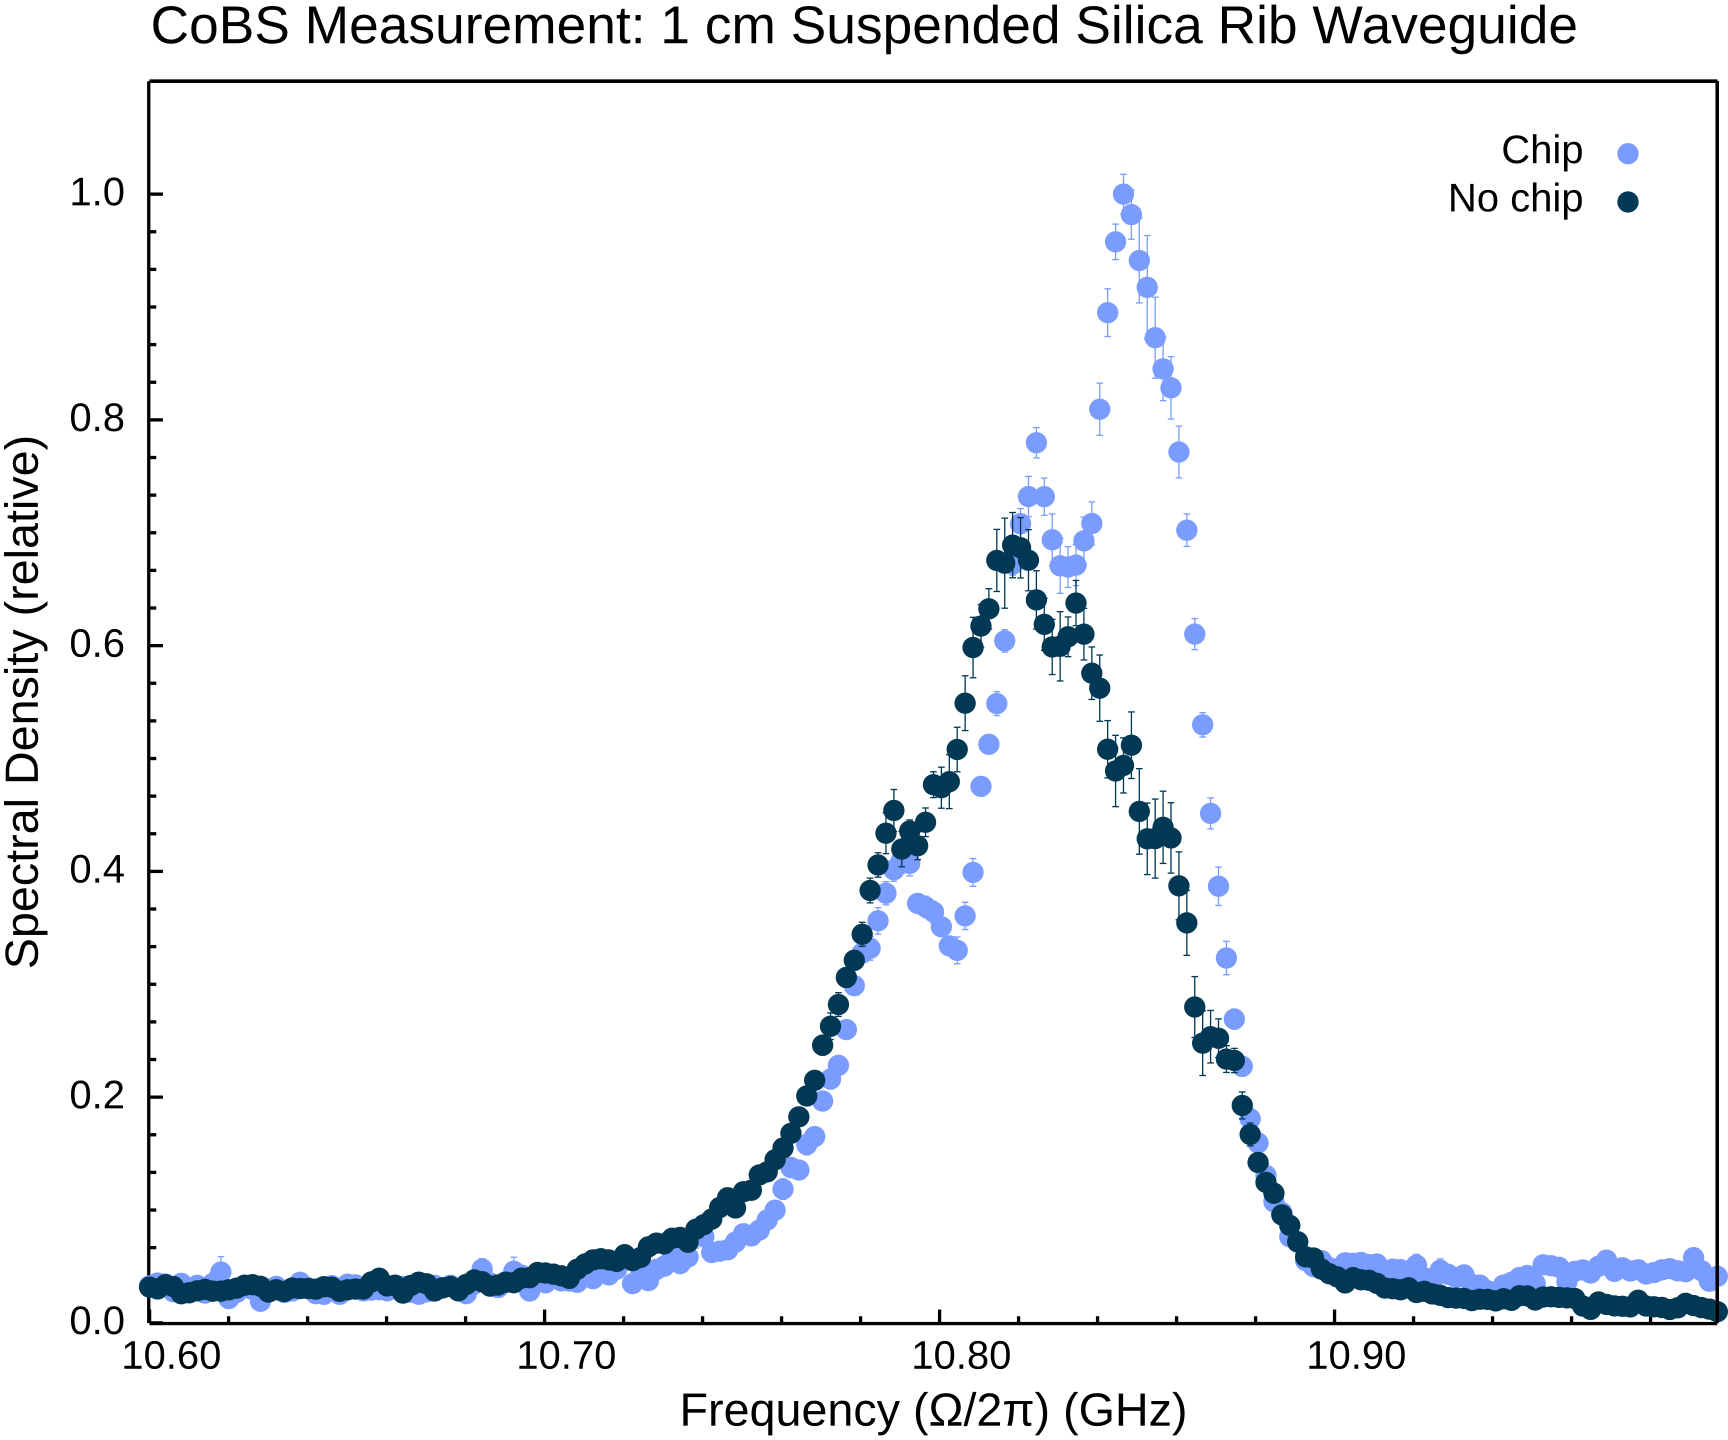
\includegraphics[width=.85\textwidth]{figs/4-Raman/CoBS Measurement: 1 cm Suspended Silica Rib Waveguide.png}
  \caption[\ac{CoBS} measurement of a suspended silica rib waveguide for a backward scattering process.]{\ac{CoBS} measurement of a suspended silica rib waveguide for a backward scattering process. A subsequent measurement with the chip waveguide removed is also plotted. The spectral response of the \ac{SMF-28} which comprises much of the sample stage of the instrument is visible without the chip, however a notable signal from the waveguide can be seen above the background. In obtaining the spectra, five repeated measurements of both the signal and background (probe off) were collected at a \SI{100}{\hertz} \ac{RBW}, dwelling for \SI{1}{\second} at each \SI{5}{\mega\hertz} frequency step. Plotted is the resulting background-subtracted spectrum. Uncertainties represent 1\(\sigma\) standard error of the mean.}
  \label{fig:Raman:August2024chipnochip}
\end{figure}

\subsection{Elastically-Suspended Photonic-Phononic Waveguide}
\label{subsec:Raman:Target:WigglyWaveguide}

In this section we provide analysis of expected optomechanical behavior from a specialized photonic--phononic waveguide designed and fabricated by the Hawkins group at \ac{BYU}. This device features a silica rib suspended on a thin memberane of elastic SU-8 polymer, primarily used as a negative photoresist which acts as a sacrificial layer in forming complex layered designs. Through collaborative discussions sharing ideas and specific domain knowledge between us and the Hawkins group, Dr. Hawkiins cleverly proposed we may see a large mechanical response from harnessing the elastic nature of the SU-8 for optomechanical interactions. In this proposed design scheme, stimulation of a breating mode in the silica rib would induce a drumhead-like mode in the SU-8 suspension. In parallel to this design behavior, we also proposed to design notches or other similar acoustic boundary feature to support acoustic guidance down the length of the waveguides. Improved acoustic guidance would produce stronger opto-mechanical interactions between light and sound along the lenth of the wavegide due to more tightly confined mode overlap (\(A_{\rm eff}^{ao}\)). These lengthwise notches or other similar feature, we proposed, might be designed to also act as lengthwise acoustic resonators. These resonant acoustic cavity notches would trap traveling-wave phonons stimulated in the silica rib and effectively produce a controllable n-multiple of short path length samples lengthwise along both sides of one chip device of desired half-coherence-length spacing. These design features were indeed implemented, and successful proof of principle elastically-suspended photonic-phononic waveguides were created and sent to us for testing.

\begin{figure}[t]
  \centering
  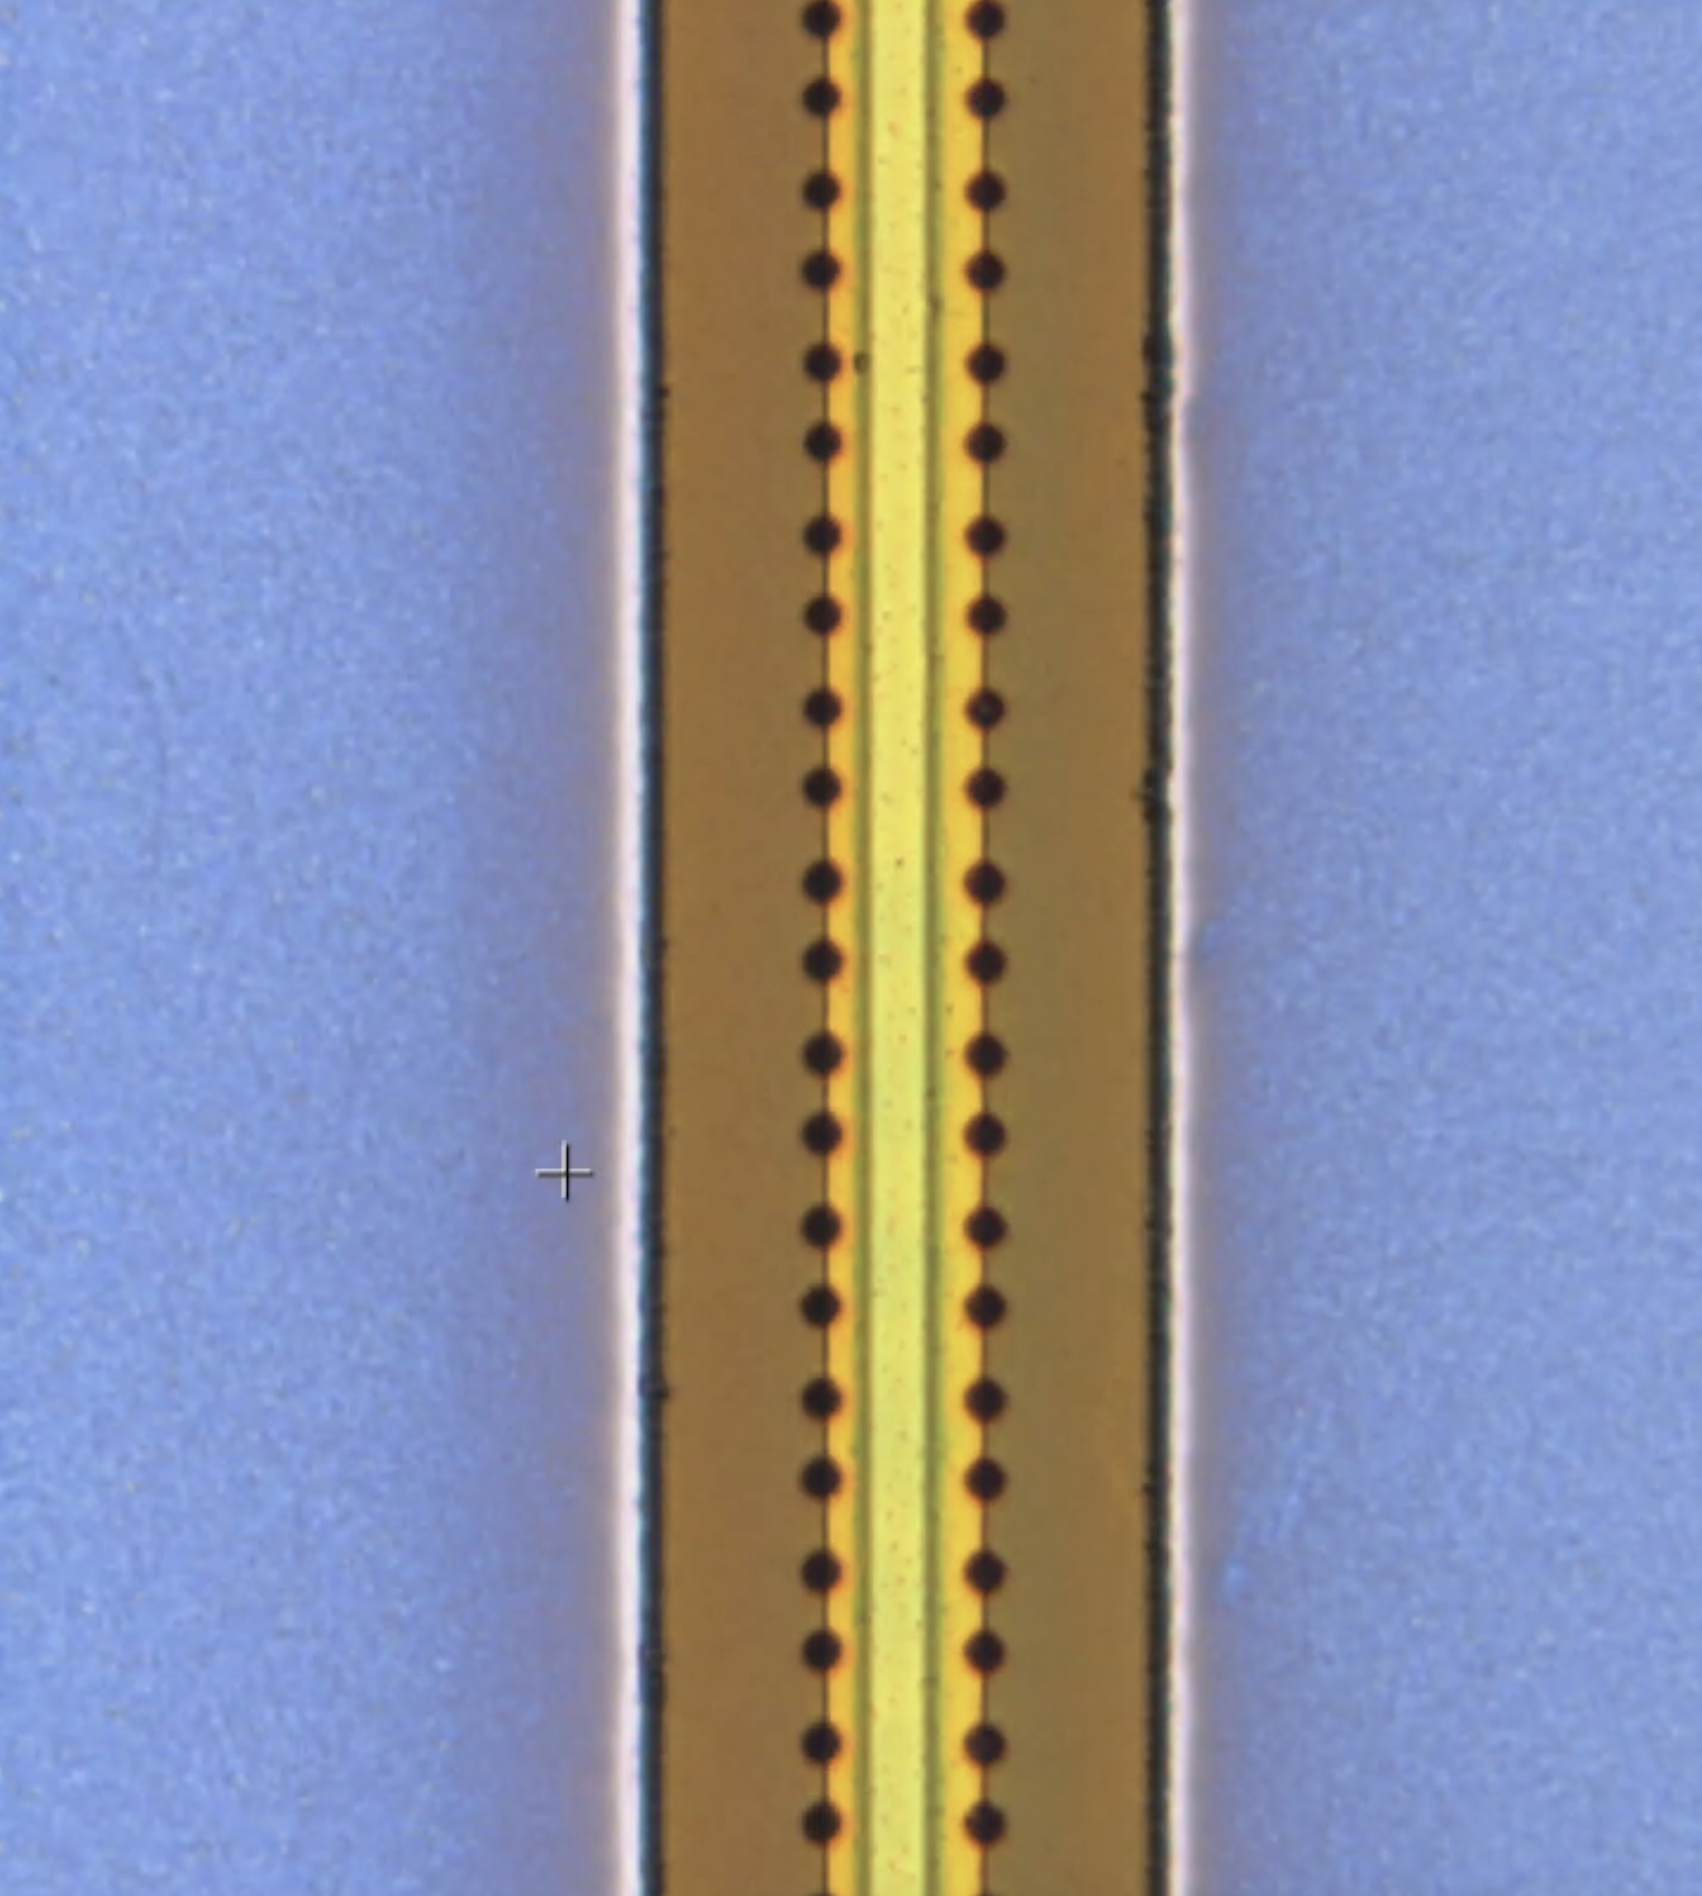
\includegraphics[width=.65\textwidth]{figs/4-Raman/wigglyWaveguideMicroscopeImage.png}
  \caption[Microscope image of the elastically-suspended phophotonic-phononic waveguide.]{Microscope image of the elastically-suspended phophotonic-phononic waveguide designed by the Hawkins group at \ac{BYU}. The brown region shows the SU-8 suspension, with the yellow region comprising the silica rib layers. The dark circles seen running lengthwise on either side of the silica rib are holes which, if made to be evenly spaced in a future design, would offer a clean n-multiplication of acoustic resonant cavities for longitudinally-traveling phonons (Brillouin-induced) to be trapped within the cavities to produce standing-wave patterns according to the effective material sound speed and hole spacing (Raman-like modes) according to Equation~\ref{eq:Raman:f_R}.}
  \label{fig:Raman:wigglyImage}
\end{figure}

\begin{figure}[t]
  \centering
  \hspace{-2em}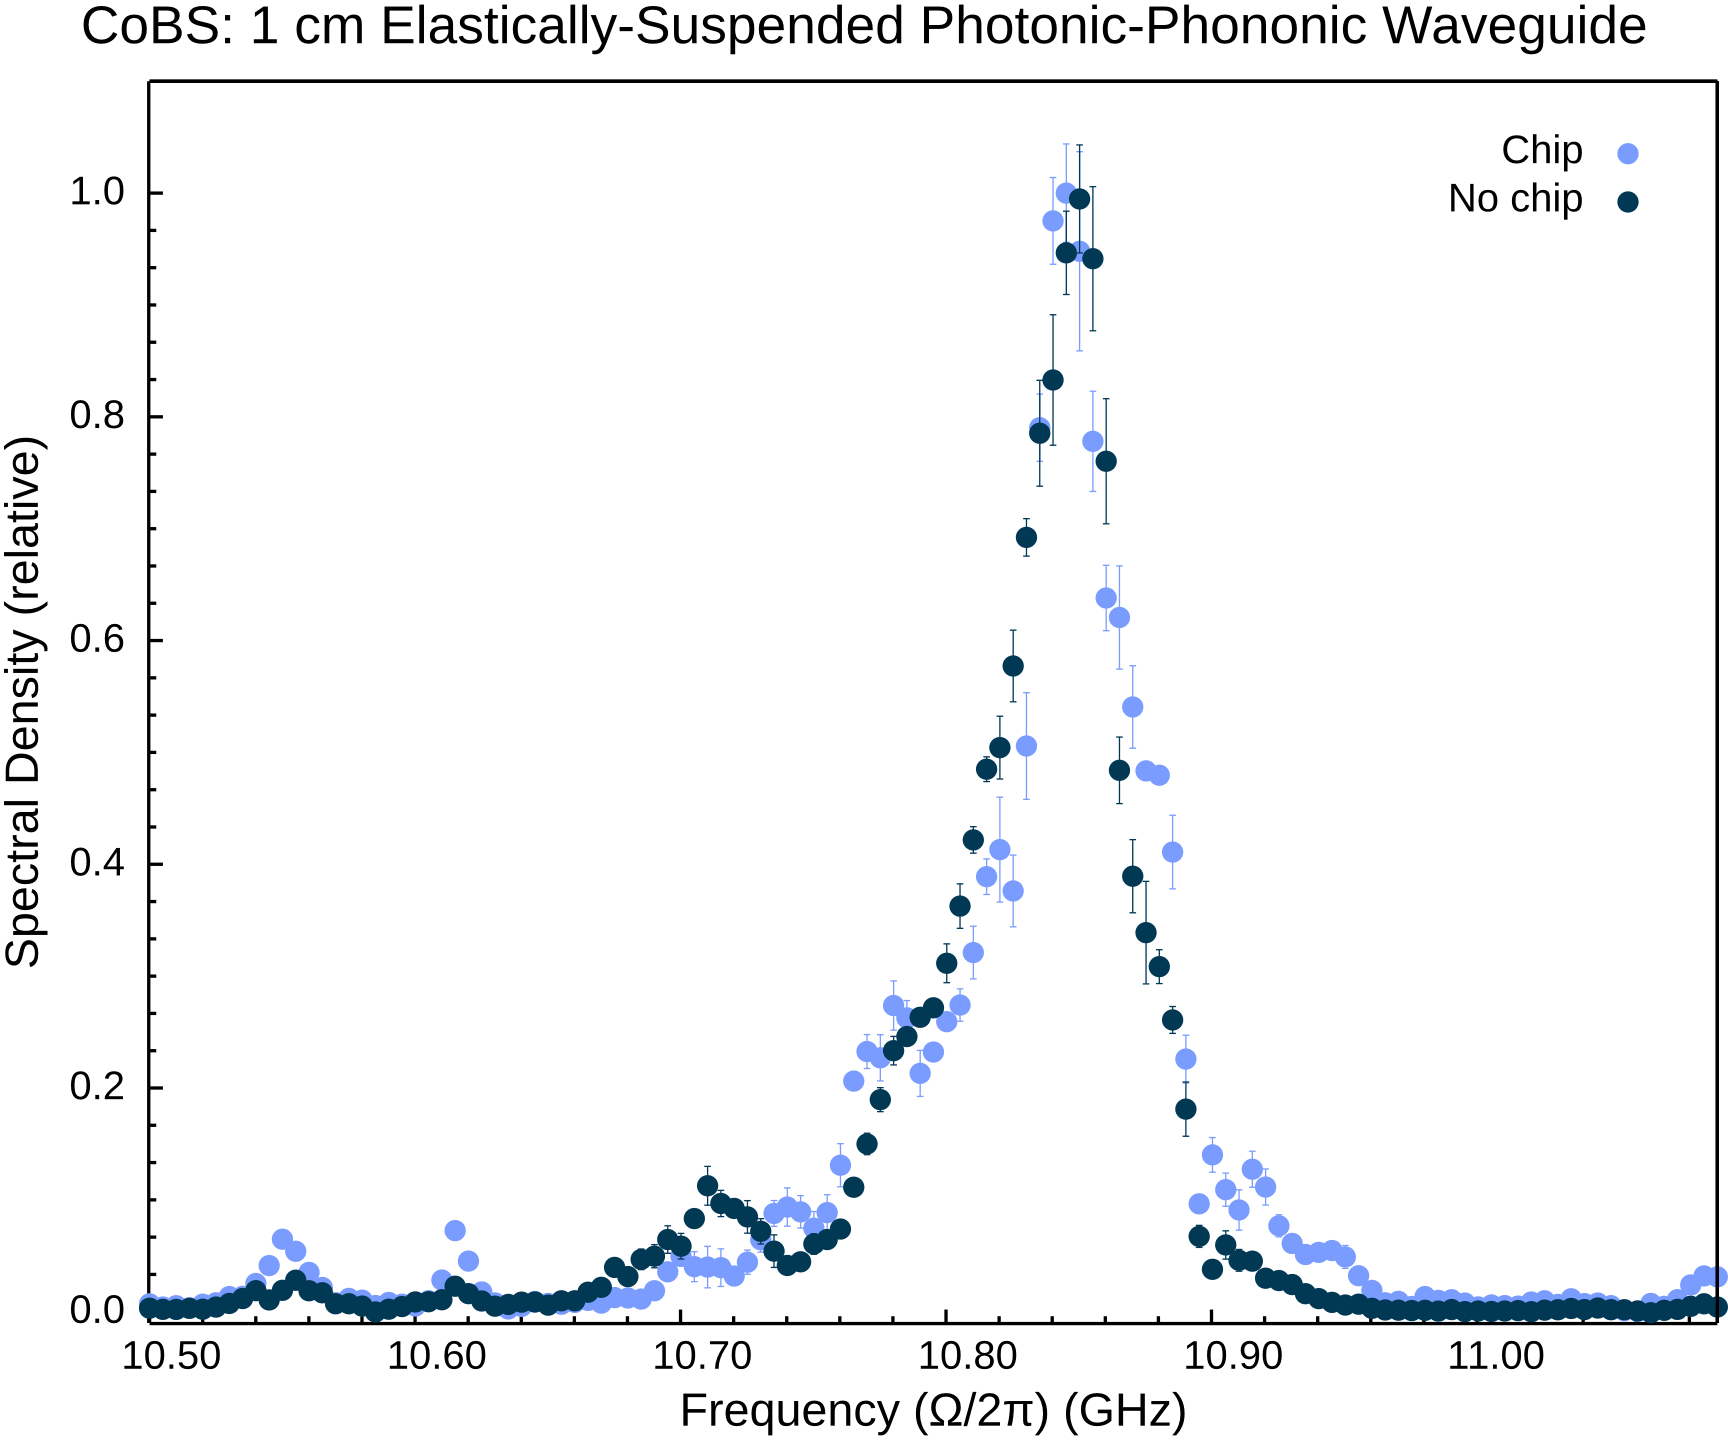
\includegraphics[width=.85\textwidth]{figs/4-Raman/CoBS: 1 cm Elastically-Suspended Photonic-Phononic Waveguide.png}
  \caption[\ac{CoBS} measurement of the elastically-suspended photonic-phononic waveguide for a backward scattering process.]{\ac{CoBS} measurement of the elastically-suspended photonic-phononic waveguide for a backward scattering process. A subsequent measurement with the chip waveguide removed reveals a similar spectral profile, as expected from the identical resonant frequency response of the \ac{SMF-28} which comprises much of the apparatus, especially in the sample region of the instrument where all three optical powers overlap. In obtaining the spectra, five repeated measurements of both the signal and background (probe off) were collected at a \SI{100}{\hertz} \ac{RBW}, dwelling for \SI{1}{\second} at each \SI{5}{\mega\hertz} frequency step. Plotted is the resulting background-subtracted spectrum. Uncertainties represent 1\(\sigma\) standard error of the mean.}
  \label{fig:Raman:wigglyCoBSspectra}
\end{figure}

Figure~\ref{fig:Raman:wigglyImage} shows a top-down microscope image of the elastically-suspended photonic-phononic waveguide device designed by the Hawkins group at \ac{BYU}. Dark circles seen running lengthwise on either side of the silica rib are holes which, if made to be evenly spaced in a future design, would offer a clean n-multiplication of acoustic resonant cavities for longitudinally-traveling phonons (Brillouin-induced) to be trapped within the cavities to produce standing-wave patterns according to the effective material sound speed and hole spacing (Raman-like modes) according to Equation~\ref{eq:Raman:f_R}. Figure~\ref{fig:Raman:wigglyCoBSspectra} plots the spectra collected from an initial test \ac{CoBS} measurement of backward Brillouin scattering in the elastically-suspended silica rib of the photonic-phononic waveguide. While some spectral features differ between the ``Chip'' and ``No chip'' measurements, additional measurements and testing are required to confirm or deny the significance of these apparent features.

In what follows, we present preliminary theoretical estimates of the key mechanical modes and optomechanical couplings predicted for the elastically-suspended photonic-phononic waveguide under development. The structure under consideration consists of a polymeric (SU-8) membrane that is tensioned during high-temperature curing and supports a rib waveguide above it. This combined membrane-and-rib geometry gives rise to multiple distinct mechanical resonances that can be excited and probed optically via the \ac{CoBS} instrument operating in the forwards scattering configuration. We summarize below the principal modes, referred to as ``drumhead'' modes for the membrane and ``breathing'' modes for the rib, and estimate rough frequency ranges in which they are expected to appear. We first consider the rib portion of the waveguide, having characteristic lateral width and thickness of \SI{4}{\centi\meter} and \SI{6}{\centi\meter}, respectively. One can treat the smallest cross-sectional dimension, denoted \(d\), as setting the approximate half-wavelength condition for its fundamental breathing mode. The simplest estimate for such a half-wavelength mechanical resonance is given equivalently by Equation~\ref{eq:Raman:f_R}, restated here as

\begin{equation}
f_{\rm rib,breathe} \approx \frac{v_{\rm s}}{2d},
\end{equation}
\\
where \(v_{\rm s}\) is the speed of sound in the silica rib and \(d\) is the lateral width. Taking the rib to be \SI{6}{\micro\meter} wide and assuming a speed of sound in the range \SI{5}{\kilo\meter\per\second} to \SI{6}{\kilo\meter\per\second}, this places the fundamental rib breathing mode near several hundred \si{\mega\hertz} (estimates range from \SI{400}{\mega\hertz} to \SI{500}{\mega\hertz}). Higher-order modes can arise (integer multiples of the half-wavelength condition), and so in practice one expects a series of possible breathing modes in the 100s of \si{\mega\hertz} to low-\si{\giga\hertz} range.

\begin{figure}[t]
  \centering
  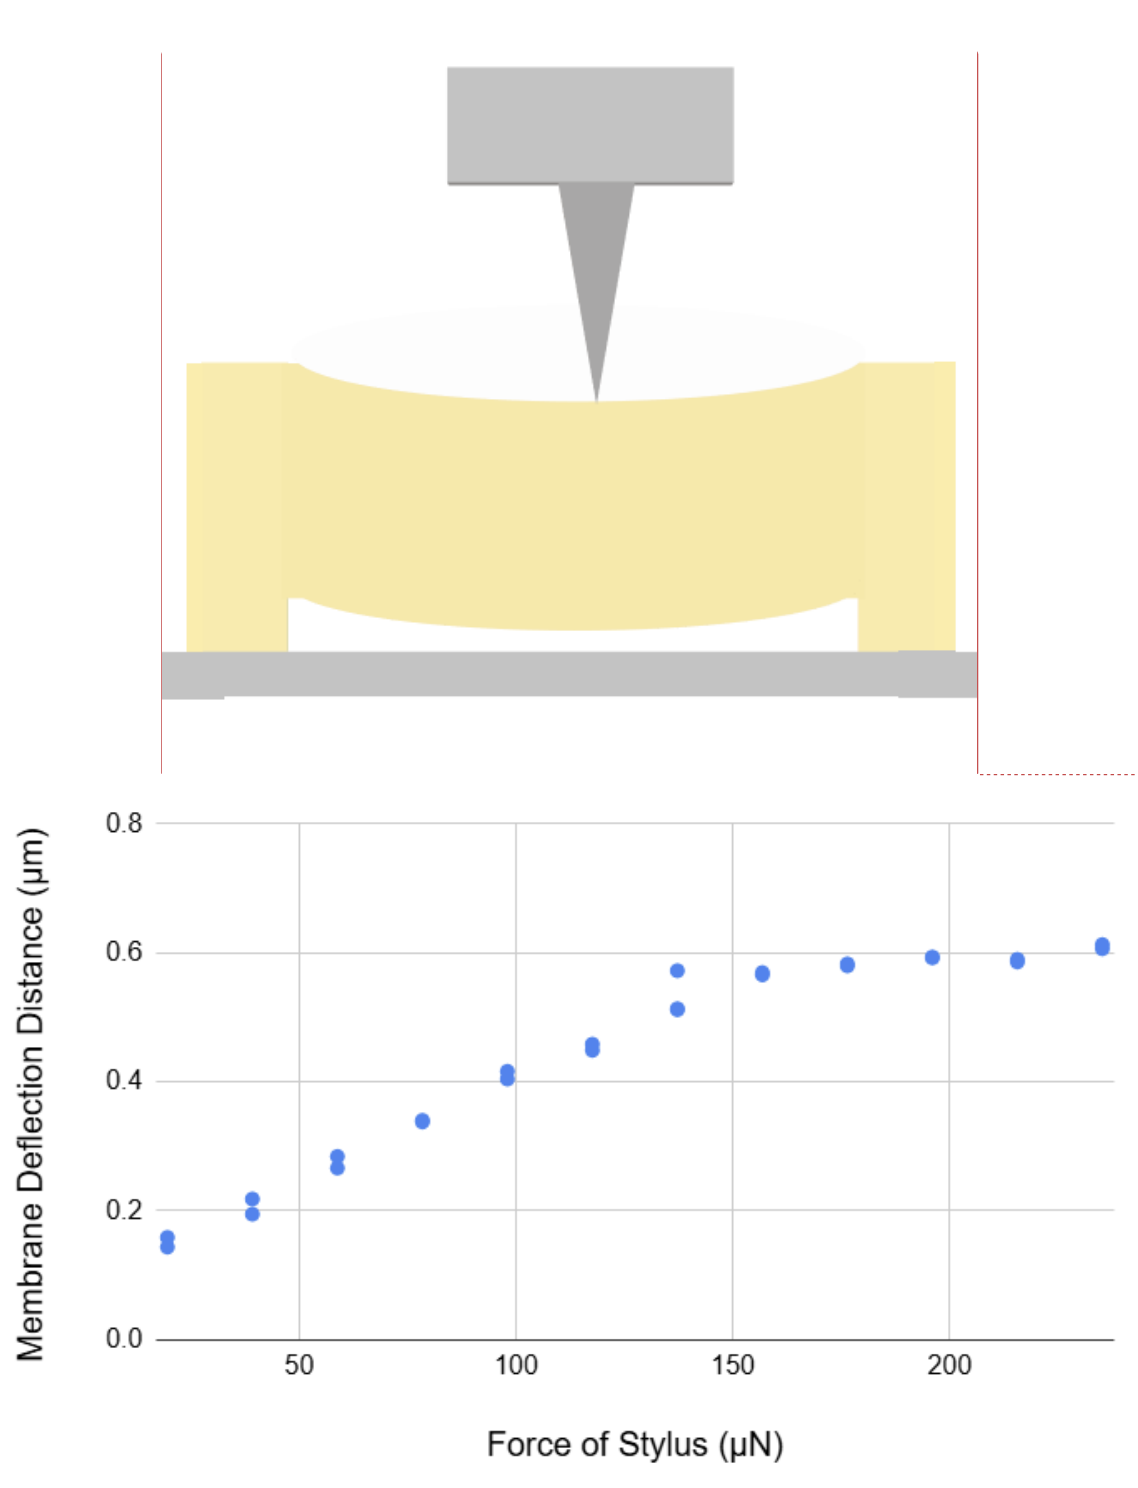
\includegraphics[width=0.61\textwidth]{figs/4-Raman/profilometer.png}
  \caption[Needle profilometer force-deflection measurements performed on the suspended polymer membrane of the photonic-phononic waveguide.]{Needle profilometer force-deflection measurements (illustrated above) performed on the suspended polymer membrane of the photonic-phononic waveguide. The inverse slope of the data (taken to be linear) is proportional to the tension of the membrane (\(m\propto T\)). Using \(m \approx\) \SI{300}{\newton\per\meter}, we estimate the tension of the membrane to be \(T \approx\) \SI{2}{\milli\newton\per\meter}, giving a transverse sound speed \(v_{\rm s} \approx\) \SI{1}{\meter\per\second} via Equation~\ref{eq:Raman:TransverseSoundSpeed}. Figure and data courtesy of Adams et al., Hawkins group, \textit{manuscript in prep}.}
  \label{fig:Raman:profilometer}
\end{figure}

In principle, when optically excited via the forward \ac{CoBS} process, the rib breathing mode can couple to and drive displacement of the underlying elastic polymer membrane. Conversely, membrane stimulation at or near the rib’s breathing-frequency range (according to the membrane's thickness) can induce motion in the rib. Thus, the device design permits either the drumhead mode of the membrane or the rib breathing mode to be excited (off-resonance if necessary) and potentially induce mechanical vibration in the other. Beneath the rib, the polymer membrane is suspended over an open region which has been etched away, and is anchored on either side. We thus expect a classical drumhead family of modes in which the membrane oscillates out-of-plane. The tension provided by the fabrication curing process indicates that the membrane vibrates in accordance with a tension-dominated regime. For a square membrane of dimension \(L\), under tension per unit thickness \(T\) and with mass density \(\rho\) and thickness \(h\), the fundamental frequency (1,1) can be approximated by

\begin{equation}
  f_{\rm membrane,\,drumhead\,(1,1)} \approx \frac{v_{\rm s}}{\sqrt{2}L},
  \label{eq:Raman:SquareMembrane}
\end{equation}
\\
where \(v_{\rm s}\) is the \emph{transverse} sound speed of the membrane, given by

\begin{equation}
  v_{\rm s} = \sqrt{\frac{T}{\rho_{\rm A}}} = \sqrt{\frac{\sigma h}{\rho h}} = \sqrt{\frac{\sigma}{\rho}},
  \label{eq:Raman:TransverseSoundSpeed}
\end{equation}
\\
where \(\rho_{\rm A}\) and \(\rho\) are the areal and volumetric mass density of the membrane, respectively, and \(\sigma\) is the stress on the membrane (\si{\pascal}) corresponding to the tension per unit membrane thickness (\(\sigma = T/h\)).

Modeling the polymer membrane as a square membrane, we can estimate the fundamental membrane drumhead mode using a mean density of SU-8 (\(\rho =\) \SI{1190}{\kilo\gram\per\cubic\meter}) \cite{roch2003fabrication} and needle profilometer tension measurements performed on the membrane. Figure~\ref{fig:Raman:profilometer} plots deflection for various stylus force values applied to the membrane, as measured by Adams et al. of the Hawkins group (\textit{manuscript in prep}) for the elastically-suspended photonic-phononic device under consideration. The inverse of the slope of these data (taken to be linear, \(m \approx\) \SI{300}{\newton\per\meter}) allows for the membrane's approximate tension to be found via \(T \approx \frac{L}{4}m \approx\) \SI{2}{\milli\newton\per\meter} for a square tension-dominated membrane with side length \(L\) and a small central point load. \cite{blevins1980formulas, timoshenko1959theory} For a \SI{2}{\micro\meter}-thickness with Equation~\ref{eq:Raman:TransverseSoundSpeed}, this gives an approximate transverse sound speed of a very slow \(v_{\rm s} \approx\) \SI{1}{\meter\per\second}. Inserting this into Equation~\ref{eq:Raman:SquareMembrane} with length \(L\approx\) \SI{25}{\micro\meter}, we anticipate the fundamental drumhead mode resonant frequency of the SU-8 membrane to lie around \SI{30}{\kilo\hertz}. Meanwhile, the rib breathing mode are predicted to lie around the mid-100s of \si{\mega\hertz}. Given this 4-order-of-magnitude discrepancy in resonant frequencies, the two mechanical modes are not expected to exhibit mechanical coupling, even when accounting for the possibility of off-resonant driving. To have the two resonances approach each other, one might alter the fabrication parameters to try significantly increasing the resulting tension of the membrane, perhaps by experimenting with different bake times or temperatures and membrane thicknesses. Alternatively, or additionally, shortening the length \(L\) across which the membrane spans from clamp-to-clamp would minimally nudge its resonant frequency higher.

%--------------------------------------------------------------------%

\section{Discussion}
\label{sec:Raman:Discussion}

In this chapter, we have investigated the potential for creating Raman-like vibrational modes via Brillouin interactions in a variety of photonic and phononic structures. By examining how traveling-wave phonons can be transformed into standing-wave resonances, we bridge the gap between conventional Brillouin physics (characterized by traveling acoustic phonons) and a regime reminiscent of Raman scattering (characterized by standing-wave vibrations). Our experimental and theoretical efforts illustrate both the challenges and the promising pathways for realizing stable, high-quality, Brillouin-induced Raman modes in waveguides, crystals, and fibers. Below, we synthesize the key findings and discuss future directions.

\subsection{Pathways to Brillouin-Induced Raman Modes}
\label{subsec:Raman:Pathways}

A central goal has been to identify platforms capable of generating high-\(Q\) standing-wave vibrational modes, analogous to conventional Raman-active modes, by leveraging Brillouin coupling in materials where both the optical and the acoustic (or elastic) degrees of freedom can be engineered. These results highlight how geometry, acoustic impedance contrasts, and overall device configuration govern the competition between traveling- and standing-wave phonons. Here, we group the ideal platforms by three broad categories: waveguides, \ce{TeO2} crystals, and fiber-based approaches. A promising strategy for forming Raman-like resonances emerges from waveguide geometries that confine both light and sound. Notably, rib waveguides of \ce{TeO2} (or other similar high-Brillouin-gain chalcogenide material composition) are attractive due to the high photoelastic coefficients of tellurite and chalcogenide glasses, coupled with the possibility of incorporating evenly spaced square holes to pin acoustic modes. The fabrication of a long rib waveguide on the order of centimeters can allow an extended optical interaction length while introducing a phononic band structure via an engineered hole pattern. This pattern can create a 1D phononic bandgap, effectively confining traveling-wave phonons to form standing waves at selected frequencies. Tellurite- or other chalcogenide-based waveguides combine strong Brillouin gain with a sufficiently low acoustic damping rate to enable coherent standing-wave formation at room temperature (Section~\ref{subsec:Raman:Target:TeO2}). As in earlier suspended photonic-phononic waveguides (Section~\ref{subsec:Raman:Target:WigglyWaveguide}), the tension in the membrane can significantly alter the acoustic mode spectrum. Proper design of periodic corrugations and sidewalls ensures that back-reflection of phonons gives rise to well-defined modes at the material Brillouin frequency shift. By tuning geometric parameters such as hole spacing and their proximity to the rib waveguide, it is possible to achieve a strong acousto-optic overlap while allowing the transduced traveling-wave phonons to ``spill'' out to the holes for selective Raman-like mode conversion.

Although many of our demonstrations focused on thin-films of \ce{TeO2}, a bulk or thick-crystal platform is also a compelling route for Brillouin-induced Raman effects. \ce{TeO2} boasts among the largest photoelastic coefficients for chalcogenide or oxide glasses, making it an exemplary host for strong acousto-optic coupling. In a bulk crystal with polished facets or embedded reflectors, backward Brillouin scattering may transition into a standing-wave configuration within the \ac{CoBS} sensitivity limits, allowing observable Raman-like resonances. Relative to many polymeric or silica systems, crystalline \ce{TeO2} can exhibit reduced phonon damping, particularly for carefully oriented crystal axes. This intrinsic advantage can facilitate a higher mechanical \(Q\) and a narrower linewidth (longer phonon coherence length \(L_{\rm coh}\)), key ingredients for stable Brillouin-induced Raman modes (see Table~\ref{tab:Raman:TeO2}). Realizing a clear set of discrete ``Raman-like'' lines in a bulk crystal requires controlling reflections at each interface. Spurious acoustic reflections or partial mode mismatch can excite multiple unwanted phonon branches, broadening the spectrum. Future work could integrate an acoustic Bragg grating within the crystal or deposit patterned reflectors on crystal faces to support more robust mode confinement.

Finally, optical fibers remain one of the most convenient photonic platforms for combining long interaction lengths with precise control over acoustic guidance. Introducing a series of periodic notches or refractive index modulations forms an acoustic mirror inside the fiber, providing a route to localized standing-wave phonons. Unlike conventional uniform-core fibers where traveling acoustic waves dominate, these fiber Bragg structures could reflect phonons at targeted frequencies. Once the phonon reflectivity is sufficiently high, coherent standing waves may arise. Implementing an acoustic fiber Bragg grating must balance strong reflection of phonons (to produce standing-wave modes) with minimal introduction of optical loss. While doping or microstructuring the fiber is feasible, the potential for scattering or wavefront distortion may ultimately impact optical guidance.

Collectively, these three categories (\ce{TeO2} waveguides, \ce{TeO2} crystals, and notched acoustic fibers) demonstrate overlapping yet distinct methods for accessing Brillouin-induced Raman modes. Each system can be fine-tuned for specific applications: \ce{TeO2} waveguides for integrated photonics where footprint is critical; bulk crystals for high-\(Q\) acoustic experiments; and fiber-based geometries for long-distance coupling and simpler device integration.

\subsection{Conclusion}
\label{subsec:Raman:Conclusion}

By mapping the transition from traveling-wave Brillouin phonons to standing-wave Raman-like modes across these diverse platforms, we underscore the broad adaptability of optomechanical coupling at room temperature. The demonstrations in this chapter affirm that controlling acoustic boundary conditions, whether via physical reflectors, periodic perturbations, or intrinsic interface mismatches, lies at the center of generating stable, high-\(Q\) vibrational modes. The overarching theme of the work presented in this document is control of phonons at room temperature. The progress reported here highlights that we do not need to confine ourselves exclusively to classical Raman systems or purely Brillouin-based traveling-wave scenarios. Instead, it is possible to strategically blend the strengths of each to realize new types of hybrid resonances with unique spectral signatures. Ultimately, these Brillouin-induced Raman modes broaden the scope of optomechanical interactions. They show that even modest structural modifications, whether in waveguides, bulk crystals, or specialized fibers, can tip the balance away from purely traveling acoustic waves toward fully resonant, discrete modes. This tunability promises new device functionalities at telecom and near-infrared wavelengths, where controlling phonons in tandem with photons stands to accelerate advances in sensing, signal processing, and quantum photonics.

\clearpage
\thispagestyle{empty}
\null
\newpage
